\documentclass[a4paper,12pt,openright,titlepage,oneside]{book}

%\usepackage[english,brazil]{babel} 
%define regra de gramática para separar síbalas {babel}
%e altera os títulos (como chapters, sections, references) para português
%\usepackage[portuguese,brazil]{babel} 
%\usepackage[portuges]{babel}
%Altera os títulos (como chapters, sections, references) para português
%\usepackage[brazil]{babel}   
\usepackage[brazilian]{babel}
%permite digitar caracteres acentuados no texto, no lugar de usar códigos
\usepackage[utf8]{inputenc} 
%permite copiar texto acentuado no PDF gerado
\usepackage[T1]{fontenc}

%Comentários de múltiplas linhas
%\begin{comment} 
%blablabla 
%blabla
%\end{comment}

%Acesso aos dados do documento como autor, título e data por meio dos comandos \MyAuthor, \MyTitle e \MyDate
%Download do pacote em http://tug.ctan.org/tex-archive/macros/latex/contrib/authoraftertitle/
%O mesmo foi extraído na pasta da dissertação
\usepackage{authoraftertitle}

%Permite fazer controle de alterações (destacando alterações) em documentos tex
%http://www.ctan.org/tex-archive/macros/latex/contrib/changes
%\usepackage{changes}

%Habilitar o parâmetro final apenas quando for ser gerada a versão final do documento (sem os destaques de alterações).
%Tal parâmetro deve ser incluído ou removido do \usepackage anterior
\usepackage[final]{changes}


\usepackage{verbatim} % http://devdaily.com/blog/post/latex/multi-line-comments-in-latex-begin-123-comment-125-verbatim

%permite colocar um determinado trecho de texto em orientação paisagem (landscape)
%http://texblog.wordpress.com/2007/11/10/landscape-in-latex/
%uso: \begin{landscape} blablabla \end{landscape}
\usepackage{lscape}

\usepackage{caption}
\usepackage{nomencl} %pacote para gerar lista de abreviações - http://franz.kollmann.in/latex/latex.html
\usepackage{epsfig} %usar formato de figura .eps
\usepackage[utf8]{inputenc} %definir que vai trabalhar com codificacão utf8 e inputenc -> entrada de acentos normal
\usepackage{colortbl}
\usepackage[lmargin=3.0cm, rmargin=2.50cm, tmargin=2.50cm, bmargin=2.50cm]{geometry} %define as margens
\usepackage{array}
\usepackage{subfigure}
\usepackage{amsfonts}
\usepackage{amstext}
\usepackage{amsmath}
\usepackage{amssymb}
\usepackage[thmmarks,amsmath]{ntheorem}%\usepackage{amsthm}
\usepackage{boxedminipage}
\usepackage{geometry}
\usepackage{theorem}
\usepackage{fancybox}
\usepackage{enumerate}
\usepackage{fancyhdr}
\usepackage{ifthen}
\usepackage{multirow}
\usepackage{times}
\usepackage{afterpage}
\usepackage{color}
\usepackage{colortbl}
\usepackage{rotating}
\usepackage{makeidx}
\usepackage{indentfirst}
\usepackage{epigraph}
\usepackage{amsmath}
\usepackage{latexsym}
\usepackage{setspace}
\usepackage[notlof,notlot,nottoc]{tocbibind}
\usepackage{template-FT-UnB/ft2unb}

\usepackage{listings}  
%\usepackage{listingsutf8} 


\sloppy %formata o texto de forma justificado

%----------------DEFINE FORMA CORRETA DE HIFENIZAÇÃO PARA ALGUMAS PALAVRAS ----------------
\hyphenation{cons-tru-a}
\hyphenation{e-xem-plo}
\hyphenation{e-xem-plar}
\hyphenation{e-le-men-to}
\hyphenation{e-le-men-tar}
\hyphenation{ma-nu-al}
\hyphenation{res-pos-ta}
\hyphenation{Li-li-ssa-nne}
\hyphenation{ca-rac-te-ris-ti-ca}
\hyphenation{ca-rac-te-ris-ti-cas}
\hyphenation{ca-rac-te-ris-ti-co}
\hyphenation{ca-rac-te-ris-ti-cos}
\hyphenation{cor-res-pon-den-ci-as}
\hyphenation{cons-tru-am}
\hyphenation{re-a-li-za-da}
\hyphenation{re-a-li-za-do}
\hyphenation{re-a-li-za-das}
\hyphenation{re-a-li-za-dos}
\hyphenation{i-ne-xis-ten-cia}
\hyphenation{i-ne-xis-te}
\hyphenation{e-xis-te}
\hyphenation{di-fe-ren-te}
\hyphenation{di-fe-ren-tes}
\hyphenation{dei-xan-do}
\hyphenation{ins-ta-la-do} 
\hyphenation{ins-ta-la-dos} 
\hyphenation{ins-ta-la-da}
\hyphenation{ins-ta-la-das}
\hyphenation{re-gis-tra-do}
\hyphenation{re-gis-tra-dos}
\hyphenation{re-gis-tra-da}
\hyphenation{re-gis-tra-das}
\hyphenation{des-cre-ve}
\hyphenation{res-pei-to}
\hyphenation{re-a-li-za}
\hyphenation{re-a-li-zar}
\hyphenation{a-tu-a-li-zar}
\hyphenation{a-tu-a-li-zan-do}
\hyphenation{a-tu-a-li-za-do}
\hyphenation{a-tu-a-li-za-da}
\hyphenation{fun-ci-o-na-li-da-de}
\hyphenation{pos-si-bi-li-da-de}
\hyphenation{dis-po-si-ti-vo}
\hyphenation{dis-po-si-ti-vos}
\hyphenation{e-xis-te}
\hyphenation{e-xis-tir}
\hyphenation{des-co-ber-ta}
\hyphenation{des-co-ber-to}
\hyphenation{de-sig-nar}
\hyphenation{de-sig-na-do}
\hyphenation{o-pe-ra-ci-o-nais} 
\hyphenation{o-pe-ra-ci-o-nal}
\hyphenation{con-si-de-ra-do}
\hyphenation{con-si-de-ra-dos}
\hyphenation{ou-tro}
\hyphenation{ou-tra}
\hyphenation{ou-tros}
\hyphenation{ou-tras}
\hyphenation{e-xis-ten-te}
\hyphenation{e-xis-ten-tes}
\hyphenation{LuaOnTV}
\hyphenation{De-fi-ni-tion}
%------------------------------------------------------------------------------------------

\usepackage{hyperref}
\usepackage{url}

\usepackage{graphicx}
\DeclareGraphicsExtensions{.jpg,.pdf,.mps,.png,.gif,.eps}
\graphicspath{{../images/}} %define diretório de imagens

%% Define a new 'leo' style for the package that will use a smaller font.
\makeatletter
\def\url@leostyle{%
  \@ifundefined{selectfont}{\def\UrlFont{\sf}}{\def\UrlFont{\small\ttfamily}}}
\makeatother
%% Now actually use the newly defined style.
\urlstyle{leostyle}

% Existe outra diretiva, mais abaixo, que define outro estilo, de nome abnt-num
% O uso de mais de um estilo está gerando um warning na compilação.
% \bibliographystyle{plain} 

%line-numbers, inputencoding=utf8/latin1
%Define o estilo para listagens de código fonte
\lstset{
  numbers=left, %numeração de linhas à esquerda
  stepnumber=1,
  firstnumber=1,
  numberstyle=\tiny,
  extendedchars=true,
  frame=none,
  basicstyle=\footnotesize,
  stringstyle=\ttfamily,
  showstringspaces=false,
  %language=Java, %deve ser definida na inclusão de cada trecho de código, pois podem existir linguagens diferentes em exemplos diferentes
  breaklines=true,
  breakautoindent=true,
  %estilos de comentário de uma e várias linhas
  morecomment=[l]{--}, morecomment=[s]{/*}{*/}, morecomment=[s]{<!--}{-->}, morecomment=[s]{--[[}{--]]}
}


%\begin{tabular}{>{\raggedright}p{0.18\linewidth}>{\raggedright}p{0.38\linewidth}>{\raggedright\arraybackslash}p{0.38\linewidth}}

\makenomenclature %Necessário para gerar lista de siglas

\title{Arquitetura orientada a serviços para comércio eletrônico no Sistema Brasileiro de TV Digital}
\titulolinhai{Arquitetura orientada a serviços}
\titulolinhaii{para comércio eletrônico no}
\titulolinhaiii{Sistema Brasileiro de TV Digital}

\author{Manoel Campos da Silva Filho}
\autori{Manoel Campos da Silva Filho}
\autorendereco{Universidade de Brasília, Faculdade de Tecnologia, Departamento de Engenharia Elétrica, 70910-900, Brasília-DF, Brasil.}

\grau{Mestre}
\area{Engenharia Elétrica}  
\siglaarea{ENE}
\tipodemonografia{Dissertação}
\programa{Mestrado}

\date{2011-06-16} %data da defesa
\dia{16}\mes{Junho}\ano{2011}

\numpublicacao{439/2011}
\siglapublicacao{PPGENE.DM}%Programa de Pós Graduação em ENgenharia Elétrica.Dissertação de Mestrado
\totalpgs{107}

\membrodabancai{Prof. Dr. Paulo Roberto de Lira Gondim, ENE/UnB}
\membrodabancaifuncao{Orientador}
\membrodabancaii{Prof. Dr. Divanilson Rodrigo Campelo, ENE/UnB}
\membrodabancaiifuncao{Examinador interno}
\membrodabancaiii{Prof. Dr. Díbio Leandro Borges, CIC/UnB}
\membrodabancaiiifuncao{Examinador externo}

\begin{document}

\pdfbookmark[0]{Agradecimentos}{agradecimentos}% * indica para nao adicionar numeracao ao titulo
\chapter*{Agradecimentos}

Gostaria de agradecer primeiramente
ao Instituto Federal de Educação, Ciência e Tecnologia do Tocantins (IFTO),
instituição onde leciono, por ter me liberado por dois anos
para cursar o programa de mestrado em Engenharia Elétrica
da Universidade de Brasília; à CAPES pela ajuda financeira
durante este período; e um agradecimento
especial a meus grandes amigos e companheiros (em ordem alfabética) 
Cláudio Monteiro, Helder Cleber, Leandro Vaguetti, Lilissanne Marcelly, Maurício Júnior, Vanice Cunha e Vinícius Rios,
que tornaram esta jornada menos cansativa e mais divertida, que foram amigos
de todas as horas, tanto nas de alegria quanto nas de tristeza.
Por fim, e não menos importante, gostaria de agradecer a meu orientador, o professor Paulo 
Gondim, por todos os ensinamentos e apoio durante esta jornada.


\chapter{Resumo}

% Acesso ao comando \MyTitle devido ao uso do pacote authoraftertitle
\section*{\MyTitle} % * é pra não numerar a seção

\replaced{Esta}{A presente} dissertação descreve uma arquitetura orientada a serviços para provimento de comércio eletrônico
pela TV Digital, por meio do Sistema Brasileiro de TV Digital (SBTVD),
desenvolvida para o sub-sistema Ginga-NCL do \textit{middleware} Ginga.
A arquitetura proposta utiliza serviços de diferentes provedores (nas áreas de telecomunicações, logística e outros) para compor 
uma estrutura de \textit{T-Commerce}. Tais serviços são desenvolvidos
considerando aspectos de interoperabilidade, utilizando o protocolo SOAP,
para o qual é apresentada uma implementação, juntamente com o
HTTP, como base para o desenvolvimento de toda
a arquitetura e um dos objetivos principais do projeto.

Com a arquitetura elaborada, uma aplicação cliente, desenvolvida
em NCL e Lua, é apresentada como prova de conceito do uso das
implementações dos protocolos e da arquitetura proposta.
Tal aplicação utiliza o \textit{framework} LuaOnTV para a construção
da interface gráfica de usuário para a TV Digital, o qual foi estendido
neste trabalho, com as melhorias sendo apresentadas ao longo do mesmo.

O trabalho ainda apresenta um conjunto de aplicações desenvolvidas a partir
dos \textit{frameworks} construídos, que complementam as funcionalidades da aplicação
de T-Commerce, como leitor de RSS e rastreamento de encomendas.

A partir do ambiente de desenvolvimento montado para a construção das aplicações, 
contendo a implementação de referência do sub-sistema Ginga-NCL do \textit{middleware} Ginga, 
nativamente instalada, foi gerada uma distribuição Linux que permite que tal ambiente
seja instalado em qualquer computador ou máquina virtual, para permitir o desenvolvimento
de arquitetura semelhante ou extensão da arquitetura proposta.



\textbf{Palavras-chave:} SBTVD, Ginga, Ginga-NCL, \textit{Web Services}, HTTP, SOAP, SOA, Lua, NCL, NCLua, NCLua HTTP, NCLua SOAP, LuaOnTV 2.0, 
\textit{E-Commerce}, \textit{T-Commerce}

\chapter{Abstract}

\section*{Service-oriented architecture for electronic commerce in the Brazilian Digital Television System}

\replaced{This}{The current} dissertation describes a service-oriented architecture for providing of digital TV electronic commerce, 
through the Brazilian Digital Television System,
developed to the Ginga-NCL sub-system of the Brazilian Ginga middleware.
The proposed architecture uses services from distinct providers
(at telecommunication, logistics and other areas) to compose a T-Commerce structure. 
Such services are developed considering interoperability aspects,
using the SOAP protocol, for wich is presented
an implementation, together with the HTTP protocol, as a basis
for the development of the entire architecture and 
one of the project main goals.

With the \replaced{architecture designed}{elaborated architecture}, a client application, developed
in NCL and Lua languages, is presented \replaced{as}{how} a proof of concept
of the protocols implementations and proposed architecture use.
Such application uses the LuaOnTV framework to build
a Digital TV graphical user interface, wich was extended in this dissertation, with the improvements being presented along it.

The work also presents a set of applications developed from
the constructed frameworks that complement the T-Commerce application functionalities, 
such as RSS reader and orders tracking.

From the mounted development environment for applications building,
containing the reference implementation of the  Ginga-NCL sub-system of the Ginga middleware,
natively installed, a Linux distribution was generated that enables such environment
to be installed on any computer or virtual machine, to allow the development
of similar architecture or extension of the proposed \replaced{one}{architecture}.


\textbf{Keywords:} ISDB-TB, Ginga, Ginga-NCL, Web Services, HTTP, SOAP, SOA, Lua, NCL, NCLua, NCLua HTTP, NCLua SOAP, LuaOnTV 2.0, 
E-Commerce, T-Commerce


\pdfbookmark[0]{Sumário}{sumario}\sumario
\pdfbookmark[0]{Lista de Figuras}{listafiguras}\listadefiguras
\pdfbookmark[0]{Lista de Tabelas}{listatabelas}\listadetabelas
\pdfbookmark[0]{Lista de Códigos Fonte}{listacodigosfonte}\listadecodigosfonte

%\renewcommand{\nomname}{LISTA DE TERMOS E SIGLAS} %Define um caption à lista de siglas
%Inclui a lista de siglas 
%Para alterar a palavra "Nomenclature" adicionada como título para a lista de siglas, 
%edite o arquivo /usr/share/texmf-texlive/tex/latex/nomencl/nomencl.sty
%alterando a linha \def\nomname{Nomenclature} para, por exemplo, \def\nomname{Siglas},
%ou mais facilmente, incluindo o comando \renewcommand{\nomname}{SIGLAS} antes de incluir a lista de siglas no documento tex
\pdfbookmark[0]{Lista de Termos e Siglas}{nomenclatura}\printnomenclature[2.5cm] 

\mainmatter %Inicia a numeracao normal cardinal
\setcounter{page}{1} \pagenumbering{arabic} \pagestyle{plain}

\chapter{Introdução} \label{cap:introducao}
Nas últimas décadas, observou-se uma evolução gradual das tecnologias da informação, e como desdobramento desse evento, a organização e o comportamento humano \replaced{sofreram}{sofrem} modificações. 
Prova disso são os sistemas de compras pelas redes de computadores, que nos últimos tempos tiveram um crescimento acelerado. 
O Brasil, assim como outros países pelo mundo, possui vários casos de sucesso
de lojas de comércio eletrônico (\textit{E-Commerce})\nomenclature{E-Commerce}{Comércio Eletrônico}\footnote{\url{www.americanas.com.br}, \url{www.submarino.com.br}, \url{www.pontofrio.com.br} e outros}.

Esse fato se deve à comodidade de, a partir de um computador ligado à \textit{Internet},  poder-se realizar compras de bens e serviços.  
Nesse modelo, o usuário tem a facilidade e a liberdade de se usar o tempo que julgar necessário para avaliar o produto que deseja adquirir, além de efetuar pesquisas em várias lojas ao mesmo tempo.

Outro fator importante, está na qualidade do atendimento, devido aos atendentes possuírem em mãos um sistema de informação para prover respostas ágeis e credenciadas. Assim, o usuário economiza tempo e se exime de problemas naturais da organização contemporânea como: as filas, gastos de deslocamento, trânsito e estacionamento.

Além disso, as lojas virtuais possuem sistemas de recomendação de produtos, que com base no perfil e nas aquisições habituais do usuário, oferecem produtos incentivando o usuário a utilizar o \textit{E-Commerce}.  Todos esses benefícios são alguns dos fatores de sucesso
das maiores lojas de \textit{E-Commerce} no Brasil e no mundo.

A Pesquisa sobre o Uso das Tecnologias de Informação
e Comunicação no Brasil/TIC Domicílios em 2009 (última divulgada até a data de finalização desta dissertação)\cite{tic2009},
realizada pelo Centro de Estudos sobre as Tecnologias da Informação e da Comunicação (CETIC.br)
\footnote{Vinculado ao Núcleo de Informação e Coordenação do Ponto BR (NIC.br)}
\nomenclature{NIC.br}{Núcleo de Informação e Coordenação do Ponto BR}
e ao Comitê Gestor da \textit{Internet} no Brasil (CGI.br)\nomenclature{CGI.br}{Comitê Gestor da \textit{Internet} no Brasil}
\nomenclature{CETIC.br}{Centro de Estudos sobre as Tecnologias da Informação e da Comunicação}
mostrou que, de 2008 para 2009, houve um aumento de 8\% na consulta a preços de produtos ou serviços na \textit{Internet},
passando de 44\% para 52\% em todo o Brasil, e que houve um crescimento nas compras \textit{on line} de 3\%,
passando de 16\% para 19\% nacionalmente.
A pesquisa ainda revela que, do total de domicílios pesquisados em 2009,
32\% tinham computador (contra 25\% em 2008) e 25\% tinham acesso à \textit{Internet} (contra 18\% em 2008).

Assim os dados da pesquisa supracitada mostram que, no Brasil, as buscas por produtos e serviços na \textit{Internet} é crescente e que gradualmente mais 
pessoas têm acesso ao comércio eletrônico. 

\deleted{
Apesar desse cenário favorável, temos que ressaltar a existência de diversos perigos nas compras via \textit{Internet}. As questões de segurança são vistas como grande entrave à plena execução dessa modalidade de compras, devido às atividades criminosas que visam ganhar dinheiro ilegalmente dentro do sistema.}

\deleted{
Esses perigos são potencializados com atividades
como as de \textit{phishing}, onde um criminoso
tenta assumir a identidade de uma empresa,
enviando mensagens eletrônicas a usuários
em nome daquela, ou mesmo
clonando o \textit{site} da empresa para tentar
enganar os usuários. Estes, ao acessarem
tais \textit{sites}, pensam estar acessando o \textit{site}
da empresa, passando a fornecer dados pessoais
como \textit{login}, senha e números de cartões de crédito,
que são capturados pelo criminoso.
}

\deleted{
Contudo, as vantagens do comércio eletrônico ainda superam os riscos e é importante ressaltar que parte de tais problemas poderia ser resolvida com atitudes preventivas do próprio usuário, como apresenta a Cartilha de Segurança
para \textit{Internet}%\footnote{\url{http://cartilha.cert.br}}
do Centro de Estudos, Resposta e Tratamento de Incidentes de Segurança no Brasil (CERT.br)
%\nomenclature{CERT.br}{Centro de Estudos, Resposta e Tratamento de Incidentes de Segurança no Brasil}.
}


O comércio eletrônico possui outros suportes além do computador, tais como o celular e, mais recentemente, a TV digital. 
A compra de produtos pela TV não é algo novo. Atualmente existem
até canais específicos para tal atividade, no entanto, o usuário
precisa utilizar um outro canal para finalizar o processo de compra.
A TV Digital traz a facilidade de permitir que todo este processo
seja iniciado e finalizado diretamente do controle remoto da TV,
trazendo mais comodidade para os usuários, em uma modalidade
denominada \textit{T-Commerce}\nomenclature{T-Commerce}{Comércio pela TV Digital}.

As possibilidades dos recursos de interatividade da TV Digital (TVD) são 
\replaced{inúmeras}{praticamente infinitas}, dependendo da criatividade das produtoras de conteúdo
e desenvolvedores de \textit{software}. Um dos sonhos atualmente possíveis com as tecnologias
de TVD é a compra de produtos que estejam sendo exibidos em um programa de TV
convencional, como um tênis, uma bolsa, um quadro, ou qualquer outro.

Tendo em vista esta tendência crescente de provimento de serviços nas mais 
diversas plataformas e o sucesso de vários serviços de comércio eletrônico 
no Brasil e no mundo, a presente dissertação descreve
uma arquitetura para provimento de comércio eletrônico pela TV Digital (\textit{T-Commerce}).
A arquitetura proposta é composta por diversos serviços \textit{Web} que, juntos,
agregam todos os serviços que são disponibilizados aos usuários 
dos sistemas de \textit{T-Commerce} a serem desenvolvidos a partir de tal arquitetura.
Esta arquitetura é então enquadrada como uma Arquitetura Orientada a Serviços (\textit{Service Oriented Architecture} - SOA),
voltada para o provimento de serviços de \textit{T-Commerce}.

%http://www.mc.gov.br/noticias-do-site/23013-ministerio-das-comunicacoes-participa-de-seminario-sobre-apagao-analogico
Tal arquitetura foi elaborada devido não terem sido encontrados outros trabalhos
que tratem de uma proposta de comércio eletrônico para a TV Digital.
Assim, a proposta aqui apresentada serve como base para o desenvolvimento
de aplicações de \textit{T-Commerce}, visando a popularização de serviços
de comércio eletrônico pelo Sistema Brasileiro de TV Digital.
Considerando que o sinal analógico de TV Digital está previsto
para ser desligado em 2016, segundo previsão do Ministério das Comunicações\footnote{\url{http://goo.gl/nLVnW}},
todos os brasileiros que desejarem receber sinal de TV, precisarão de um
televisor com conversor integrado ou um conversor para conectar à um televisor convencional.
Desta forma, sistemas de \textit{T-Commerce} podem ter um grande alcance.

A arquitetura proposta, elaborada a partir de requisitos funcionais e não funcionais, 
serve de base para a implementação de aplicativos para comércio eletrônico,
para o qual são também elicitados requisitos funcionais e não funcionais.
Esses aplicativos são construídos com base em um modelo 
de \textit{templates} para definir a identidade
visual da mesma, permitindo que, ao ser alterado o \textit{template}, toda
a identidade visual da aplicação seja alterada.

A arquitetura e a aplicação de \textit{T-Commerce} propostas utilizam \textit{Web Services}
para disponibilizar funcionalidades aos usuários. Desta forma, 
tal proposta vai ao encontro da também crescente tendência de integração entre
\textit{Web} e TV. Tal integração é possível por meio de protocolos de comunicação
padronizados, como o caso dos protocolos HTTP e SOAP, que neste trabalho são 
objeto de implementações específicas.

Para esta integração entre \textit{Web} e TV, apresenta-se uma proposta
de \textit{framework} de comunicação de dados que possibilita a comunicação
entre aplicações de TV Digital e serviços disponíveis na \textit{Web},
o qual tem seu emprego demonstrado não somente por meio de aplicações de \textit{T-Commerce},
mas também de rastreamento de encomendas, leitor de RSS e outras.

\added{
Um \textit{framework} é um conjunto de classes que incorporam um projeto abstrato de soluções para 
uma família de problemas relacionados\cite{johnson1988designing}. O mesmo pode ser também denominado como
arcabouço, estrutura, esqueleto, suporte e outros termos.
}

Alguns dos requisitos do aplicativo de \textit{T-Commerce} supracitado são contemplados com a extensão
do \textit{framework} LuaOnTV para permitir o uso de temas e a adaptação
automática da interface de usuário da aplicação para diferentes 
tamanhos de TV ou até mesmo em dispositivos móveis como telefones celulares.


 %input no lugar de include evita a quebra de linha inserida por este

\section{Objetivos} \label{sec:objetivos}

\subsection{Geral}

Propor e desenvolver uma arquitetura orientada a serviços,
por meio de \textit{Web Services} SOAP, para provimento de comércio eletrônico
pela TV Digital, favorecendo a convergência \textit{Web}-TV. 

\subsection{Específicos}

Como objetivos específicos, \replaced{propõe-se}{pretende-se}:
\begin{enumerate}[A)]
  \item \added{elicitar requisitos funcionais e não funcionais a serem atendidos por} \deleted{propor} 
  uma arquitetura baseada em padrões de serviços \textit{Web}, a ser utilizada para comércio eletrônico via TV Digital;
  
  \item \added{propor uma arquitetura de serviços de \textit{T-Commerce}, que atenda aos requisitos citados;}
  
	\item a partir da arquitetura \deleted{acima}, implementar um \textit{framework} para comunicação de dados, baseado nos protocolos HTTP e SOAP,
	para permitir a comunicação de aplicações de TV Digital, desenvolvidas nas linguagens NCL e Lua,
	que permita a interoperação com serviços \textit{Web};
	
  \item caracterizar o emprego do \textit{framework} de comunicação de dados para desenvolvimento de aplicações
  tais como Leitor de RSS, Rastreador de Encomendas, Cliente de Twitter, \added{Enquete e \textit{Quiz}};
	
	\item estender o \textit{framework} LuaOnTV\cite{junior2009luacomp} incluindo recursos
	de temas para permitir a definição centralizada das características visuais das aplicações
	desenvolvidas, além de incluir suporte a múltiplos dispositivos com diferentes resoluções
	de tela, como TV's e aparelhos celulares;
	
	\item \deleted{propor }um modelo de desenvolvimento de aplicações para TV Digital (TVD), de forma 
  que todos os formulários da aplicação (páginas/telas) tenham um mesmo
  conjunto de componentes básicos, permitindo a criação de \textit{templates} para definir a identidade
  visual da mesma. Assim, ao ser alterado o \textit{template}, toda
  a identidade visual da aplicação deverá ser alterada;
  
  \deleted{	
	%\item 
	montar uma distribuição Linux contendo a implementação de referência do sub-sistema Ginga-NCL
	do \textit{middleware} Ginga, executando de forma nativa (não virtualizada) no sistema operacional, já
	contendo todas as ferramentas necessárias e configuradas para o desenvolvimento de aplicações
	de TV Digital em NCL e Lua, permitindo o funcionamento como \textit{LiveCD} (sem necessidade de instalação
	da distribuição) ou instalando a mesma em um computador, à semelhança do realizado em \cite{soset}.
	}
\end{enumerate}


 %input no lugar de include evita a quebra de linha inserida por este
\section{Justificativa} \label{sec:justificativa}

Como o início das operações do Sistema Brasileiro de TV Digital (SBTVD) é bastante recente, onde a primeira transmissão
de sinal digital foi realizada em 2007 na cidade de São Paulo, 
até a data de elaboração da presente dissertação, só conhecia-se 
um caso de aplicação de \textit{T-Commerce} no Brasil, como citado em \cite{extra-vendas-tvd},
no qual \deleted{uma aplicação }apenas \replaced{exibem-se}{exibe} os produtos e o processo de compra deve ser realizado pelo usuário utilizando
outro canal como a loja virtual (\textit{Internet}) ou o \textit{call center} da empresa.

Além disso, tal aplicação de comércio eletrônico foi desenvolvida para 
o \textit{middleware} \textit{ByYou} (implementação do Ginga desenvolvida pela empresa TOTVS)\cite{totvs-byyou},
e seu uso fica restrito aos conversores digitais e \replaced{televisores}{TV's} que possuam
tal \textit{middleware}. Por usar API's específicas do \textit{ByYou}, a aplicação só executa em tal implementação 
do \textit{middleware} Ginga.

Como o Brasil possui diversos casos de sucesso no mercado de comércio eletrônico em larga escala, 
a disponibilização de aplicações de comércio para TV Digital é uma tendência natural,
podendo aumentar consideravelmente as vendas das empresas do ramo, devido à grande penetração
do aparelho de TV nos lares brasileiros (cerca de 96\%)\cite{ibge-pnad}, além 
de ser uma nova plataforma de \textit{E-Commerce} para os usuários.

Da falta de uma arquitetura para provimento de comércio eletrônico para o SBTVD, surgiu este trabalho
de dissertação, que apresenta uma proposta de arquitetura orientada a serviços (\textit{Service Oriented Architecture} - SOA) para a estruturação
de um ambiente de \textit{T-Commerce}. Considerando que tal arquitetura é bastante
utilizada para a integração de sistemas heterogêneos, ele vai ao encontro de um dos objetivos
do projeto: prover uma arquitetura de \textit{T-Commerce} que utilize serviços \textit{Web}
que, juntos, \deleted{contemplem tanto as exigências e padrões de qualidade das empresas quanto as necessidades e desejos dos usuários}
\added{atuem de forma interoperável com o SBTVD e os padrões W3C}.

Desta forma, como a arquitetura SOA pode, comumente, ser baseada em \textit{Web Services} SOAP, faz-se necessária
a implementação de protocolos como \textit{Hypertext Transfer Protocol} (HTTP) e 
\textit{Simple Object Access Protocol} (SOAP) em que se baseiam as tecnologias relacionadas a SOA,
sendo tais implementações \deleted{um dos }objetivos principais deste trabalho.

Com a implementação dos protocolos HTTP e SOAP (onde não se tem conhecimento, até a data de elaboração
desta dissertação, de nenhuma implementação de código aberto dos mesmos para o ambiente de TVD) criam-se enormes possibilidades
de construção de aplicações para integração entre \textit{Web} e TV, um dos objetivos deste projeto
com sua arquitetura de \textit{T-Commerce}. Como durante as pesquisas observou-se que a falta
de implementação de tais protocolos era uma queixa recorrente nos fóruns da Comunidade
Ginga no Portal do Software Público\footnote{\url{http://www.softwarepublico.gov.br/dotlrn/clubs/ginga/}}
e em outros fóruns de discussão, a implementação de tais protocolos representa uma grande contribuição
para o desenvolvimento do SBTVD. Assim, após a publicação inicial das implementações
dos protocolos HTTP e SOAP, alguns trabalhos importantes foram desenvolvidos, como será apresentado no Capítulo \ref{cap:ncluasoap}.

\section{Metodologia} \label{sec:metodologia}

Para o desenvolvimento da presente dissertação foi feito um levantamento bibliográfico
sobre as tecnologias, linguagens, ferramentas e trabalhos relacionados para nortear
a implementação da arquitetura e solução proposta.

O projeto, análise e desenvolvimento da solução seguiu o
processo de desenvolvimento em cascata juntamente com o processo de componentização\cite{sommerville2011soft}.
O processo em cascata foi adotado pois os requisitos estavam bem definidos, havendo \replaced{pequena}{pouca} probabilidade de mudanças radicais.
Já o processo de componentização foi também adotado devido ao uso de alguns componentes reutilizáveis
(como \textit{Web Services} próprios e de terceiros) realizando a integração destes diversos
componentes.

No processo de desenvolvimento em cascata, foram seguidas as seguintes etapas:
\begin{itemize}
	\item especificação de requisitos - foram definidos os requisitos funcionais e não funcionais, que são apresentados ao longo do trabalho;
	\item projeto - foi adotado o paradigma de Orientação a Objetos (OO)\nomenclature{OO}{Orientação a Objetos}, utilizando-se a \textit{Unified Modeling Language} (UML)\nomenclature{UML}{\textit{Unified Modeling Language}} para modelagem, com o auxílio de ferramenta CASE (\textit{Computer-Aided Software Engineering})\nomenclature{CASE}{\textit{Computer-Aided Software Engineering}};
	\item implementação - a implementação seguiu o paradigma OO, conforme definido na fase de projeto;
	\item testes - foram feitos testes de interoperabilidade/integração para verificar se os componentes
	da arquitetura estavam se comunicando conforme o esperado.
\end{itemize}


Optou-se, para o desenvolvimento do projeto, pelo paradigma de orientação a objetos pois o mesmo 
permite um alto grau de reutilização de código, tornando o mesmo mais organizado
e fácil de manter.

Para a comunicação entre os componentes da arquitetura da solução, foi escolhido o protocolo de comunicação SOAP, uma vez que a aplicação de TV Digital desenvolvida
faz parte de uma arquitetura distribuída e precisa realizar comunicação 
com servidores \textit{Web} por meio da \textit{Internet}. Assim, foi preciso usar um protocolo
que não tivesse problemas de bloqueio em \textit{firewalls}. Desta forma, o protocolo SOAP foi escolhido
também por ser padrão do \textit{World Wide Web Consortium} (W3C)\nomenclature{W3C}{\textit{World Wide Web Consortium}}.

Para as aplicações de TV Digital, foi escolhido o sub-sistema Ginga-NCL do \textit{middleware} Ginga
do Sistema Brasileiro de TV Digital (SBTVD)\nomenclature{SBTVD}{Sistema Brasileiro de TV Digital},
devido à grande quantidade de documentos, fóruns de discussão, ferramentas e exemplos disponíveis
em relação à outra vertente de desenvolvimento utilizando a linguagem Java no sub-sistema Ginga-J.
Considerando-se ainda que o Ginga-NCL é o único sub-sistema obrigatório para dispositivos móveis,
isto foi decisivo para a escolha, pois assim, a arquitetura e as aplicações desenvolvidas
podem, em tese, ser executadas em receptores (conversores/\textit{Set-bop Boxes}) de TV Digital fixos, móveis ou portáteis.

Com a escolha do Ginga-NCL, foi necessária a implementação do protocolo SOAP para este sub-sistema,
utilizando-se a linguagem Lua, uma vez que o primeiro só disponibiliza protocolos até a camada de transporte
do modelo OSI/ISO, como o TCP. Com isto, foi necessário realizar testes de interoperabilidade
entre aplicações de TV Digital desenvolvidas com as linguagens NCL e Lua e \textit{Web Services}
desenvolvidos em diferentes plataformas e linguagens, pois um dos grandes benefícios
do protocolo SOAP é a integração de sistemas heterogêneos. Assim, tais testes foram
necessários para garantir esta interoperabilidade.

Os requisitos da aplicação foram levantados tomando por base as funcionalidades
existentes na grande maioria dos \textit{Web sites} de comércio eletrônico
disponíveis na \textit{Internet} e bastante difundidos no Brasil.

Para a construção da interface de usuário das aplicações de TV Digital, optou-se pela utilização
do \textit{framework} LuaOnTV para abstrair as primitivas gráficas para renderização da interface.
A mesma foi projetada baseada em recursos de \textit{templates}, o que permite a personalização
e adaptação automática para diferentes resoluções de tela, tendo sido estendido
o LuaOnTV para incluir tais recursos.



\section{Organização do Trabalho}


\begin{itemize}
	\item O Capítulo \ref{cap:revisao-bib} apresenta uma revisão bibliográfica das tecnologias empregadas
e relacionadas ao desenvolvimento do trabalho.
  \item O Capítulo \ref{cap:arquitetura-tcommerce} apresenta a arquitetura de \textit{T-Commerce} proposta.
  \item O Capítulo \ref{cap:luaontv} apresenta o \textit{Framework} LuaOnTV, utilizado na construção
das interfaces gráficas das aplicações desenvolvidas.
  \item O Capítulo \ref{cap:ncluasoap} apresenta um \textit{framework} de comunicação de dados, utilizado
para a integração das aplicações desenvolvidas com serviços \textit{Web}.
  \item Por fim, o Capítulo \ref{cap:conclusao} apresenta as conclusões e trabalhos futuros.
\end{itemize}



\chapter{Revisão bibliográfica} \label{cap:revisao-bib}
\section{Comércio Eletrônico: \textit{E-Commerce}, \textit{M-Commerce} e \textit{T-Commerce}}

No início da \textit{World Wide Web} (comumente denominada apenas \textit{Web}) \nomenclature{Web, WWW}{\textit{World Wide Web}}
as primeiras páginas de \textit{Internet} possuíam apenas conteúdo estático permitindo pouca ou nenhuma interação
do usuário. A \textit{Web} era apenas um repositório de informações. Com a crescente demanda de troca
de informações entre empresas, o advento de padrões abertos de comunicação, 
e a necessidade das mesmas de alcançarem novos clientes e mercados, durante a década de 90 
começou a surgir um novo gênero de \textit{Web sites}: os \textit{sites} de comércio eletrônico\cite{chu2007evolution}.

Tais \textit{Web sites} possibilitaram a realização de negócios entre compradores e vendedores
e entre vendedores e seus parceiros. Desta forma surgiu o \textit{E-Commerce}. Este é baseado na possibilidade
de realização de transações de forma eletrônica. Segundo \cite{veijalainen2006transaction}:

\begin{quote} 
"uma transação eletrônica
é uma venda ou compra de produtos ou serviços, entre empresas, familiares, indivíduos, governos e outras organizações
públicas ou privadas, conduzidas por redes mediadas por computador."
\end{quote}

A troca de informações entre essas empresas era feita por meio de \textit{Eletronic Data Interchange} (EDI)\nomenclature{EDI}{\textit{Eletronic Data Interchange}} (troca eletrônica de informações), no entanto, isto requeria realização de acordos entre as organizações\cite{chu2007evolution},
o que poderia dificultar tais parcerias. O advento de padrões abertos como o XML permitiu a evolução
de tais processos de intercâmbio de dados e integração entre empresas.

Atualmente existem diversas empresas consolidadas na área de comércio eletrônico. Algumas nasceram na era digital
e vendem exclusivamente pela \textit{Internet}, alcançando
novos clientes e mercados nacionais e internacionais.

Com a recente popularização de dispositivos móveis e da \textit{Internet} sem fio como rede de grande abrangência (por exemplo, utilizando as tecnologias
de comunicação móvel de 3ª geração como o \textit{Universal Mobile Telecommunications System} - UMTS)\nomenclature{UMTS}{\textit{Universal Mobile Telecommunications System}}, surgem novas oportunidades para as lojas de comércio eletrônico. 
Estas entram em uma nova era, com novas perspectivas de captação de clientes e mercados. Com isto surgem novas tendências 
como o denominado Comércio Móvel (\textit{M-Commerce})\nomenclature{M-Commerce}{Comércio Móvel}, onde as transações são feitas utilizando-se dispositivos e redes de acesso móveis, tais como \textit{Wireless Local Area Networks} (WLAN's)\nomenclature{WLAN}{\textit{Wireless Local Area Network}}\nomenclature{LAN}{\textit{Local Area Network}}, redes de telecomunicações 2G ou 3G, conexões \textit{Bluetooth} ou infravermelho\cite{veijalainen2006transaction}.

Tais dispositivos móveis permitem que os usuários possam realizar compras em qualquer lugar que eles estejam,
até mesmo em suas horas livres, durante o trajeto para o trabalho, ou no horário de almoço. Desta forma,
as lojas virtuais têm um mercado em potencial para aumentar suas vendas.

Com o advento dos sistemas de televisão digital interativa e a possibilidade de se ter 
aplicativos executando juntamente com a programação áudio-visual, abre-se um
novo mercado para as lojas de comércio eletrônico: a venda de produtos pela TV.
Tais serviços de vendas pela TV não são novos, mas antes da TV Digital Interativa (TVDi),
os canais de venda pela TV apenas anunciavam produtos e os telespectadores que 
desejavam comprar um produto precisavam utilizar outro canal de comunicação, como
o telefone ou recorrer ao \textit{Web site} da loja na \textit{Internet}.
Utilizando-se os recursos da TV Digital Interativa, todo o processo de compra
pode ser realizado diretamente pelo controle remoto da TV, desde que a mesma
esteja conectada à \textit{Internet}.

As tecnologias da TV Digital trazem um novo benefício aos usuários: a possibilidade
de comprar produtos a partir de um receptor de TV Digital, caracterizando uma nova modalidade de comércio
eletrônico, denominada \textit{T-Commerce}.

Em países norte-americanos e europeus, que têm sistemas de TV Digital Interativa
há mais tempo que o Brasil, existem algumas empresas disponibilizando soluções para a área de \textit{T-Commerce}
\footnote{\url{http://www.ensequence.com/t-commerce}}
\footnote{\url{http://www.digisoft.tv/applications.html}}
\footnote{\url{http://www.icuetv.com/ets\_platform/applications/t\_commerce}}.
No Brasil, apesar de as transmissões de TV Digital terem iniciado somente em 2007 
na cidade de São Paulo\cite{inicio-transmissao-tv-digital-saopaulo}, em 2010
já \replaced{há}{haviam} soluções iniciais para \textit{T-Commerce}\cite{extra-vendas-tvd}, apesar de a finalização
da compra ainda precisar ser feita utilizando-se outros canais como o telefone.

Devido ao Brasil ser um país de características bem diferentes dos outros países, 
espera-se que a interatividade seja um grande diferencial para o país.
Como o Governo Federal pretende 
realizar inclusão social/digital por meio da TV, de acordo com o Decreto número 4.901, de 26 de novembro de 2003,
espera-se que a disponibilização de serviços pela TV seja crescente.
Um fator importante para a difusão da interatividade no país é a existência 
de aparelhos de TV em 96\% das residências\cite{ibge-pnad}, tendo grandes
possibilidades de as aplicações interativas terem um enorme público, considerando
ainda as dimensões continentais do Brasil e sua enorme população de 185.712.713 habitantes, segundo
o Censo 2010\cite{censo2010}.

Outra medida tomada pelo governo que beneficiará a interatividade pela TV Digital é a criação do 
Plano Nacional de Banda Larga (PNBL)\nomenclature{PNBL}{Plano Nacional de Banda Larga}, por meio do Decreto número 7.175, de 12 de maio de 2010,
visando prover \textit{Internet} banda larga, a um custo reduzido, em municípios onde não exista tal serviço.



\section{Sistema Brasileiro de TV Digital (SBTVD)}

O Sistema Brasileiro de TV Digital (SBTVD) atualmente é o mais
avançado do mundo. A necessidade de o Brasil implantar um sistema de TV Digital
levou o Governo Federal a emitir o Decreto 4.901, de 26 de novembro de 2003, instituindo
o referido sistema.

A partir daí, o governo passou a investir diretamente na pesquisa de tecnologias
para TV Digital. Considerando que já \replaced{havia}{haviam} outros padrões de TV Digital
no mundo, como o americano ATSC (\textit{Advanced Television Systems Committee})\nomenclature{ATSC}{\textit{Advanced Television Systems Committee}}, 
o europeu DVB (\textit{Digital Video Broadcast})\nomenclature{DVB}{\textit{Digital Video Broadcast}} 
e o japonês ISDB-T (\textit{Integrated Services Digital Broadcasting Terrestrial})\nomenclature{ISDB-T}{\textit{Integrated Services Digital Broadcasting Terrestrial}}, tais estudos concluíram que o melhor para o país seria a adoção do sistema japonês ISDB-T,
que seria estendido para atender às características e necessidades do Brasil.

Desta forma, o Decreto 5.820, de 29 de junho de 2006 estabelece o uso do ISDB-T
como base para o Sistema Brasileiro de TV Digital Terrestre (SBTVD-T)\nomenclature{SBTVD-T}{Sistema Brasileiro de Televisão Digital Terrestre}.
O decreto ainda define a criação do Fórum SBTVD (Fórum do Sistema Brasileiro de TV Digital)\footnotetext{\url{http://www.forumsbtvd.org.br}}.
Tal fórum, como menciona o decreto supracitado, tem como atribuições: 

\begin{quote}
"a assessoria acerca de políticas e assuntos técnicos referentes à aprovação de inovações
tecnológicas, especificações, desenvolvimento e implantação do SBTVD-T".
\end{quote}
 
O mesmo foi composto, como cita o decreto: 
\begin{quote}
"entre outros, por representantes do setor de
radiodifusão, do setor industrial e da comunidade científica e tecnológica"
\end{quote}

Dentre as contribuições do Brasil para a área de TVD, destaca-se a construção do Ginga\footnote{\url{http://www.ginga.org.br}}
como padrão de \textit{middleware} para aplicações interativas e não interativas.
O Ginga é uma inovação nacional, atuando como responsável
pela execução e controle do ciclo de vida das aplicações interativas, abstraindo o sistema operacional
e o hardware para elas, além de realizar tarefas especializadas como a disponibilização de \textit{Application Programming Interfaces} (API's) para
facilitar o desenvolvimento de aplicações interativas\cite{soares2009programando}.

O Ginga é composto por dois sub-sistemas: um para a execução de aplicações declarativas, denominado
Ginga-NCL\footnote{\url{http://www.gingancl.org.br}}, e outro para execução de aplicações procedurais, 
denominado Ginga-J\footnote{\url{http://dev.openginga.org}}.
Aplicações declarativas são aquelas implementadas utilizando-se uma linguagem declarativa, como
XML, de forma não algorítmica, apenas declarando elementos que comporão a mesma.
Tais linguagens abstraem muitos detalhes do desenvolvedor. 
Aplicações procedurais são aquelas implementadas utilizando uma linguagem procedural, como Java,
onde o desenvolvedor precisa escrever um algoritmo e especificar cada operação a ser realizada,
necessitando de conhecimento em linguagens de programação.

O sub-sistema Ginga-NCL permite a construção de aplicações declarativas por meio da linguagem NCL,
a \textit{Nested Context Language}\nomenclature{NCL}{\textit{Nested Context Language}}\footnote{\url{http://www.ncl.org.br}}. 
Esta é conhecida como uma linguagem de cola, que permite criar aplicações declarativas
juntando-se diferentes tipos de mídias como imagens, texto, hipertexto (HTML), vídeos
e outros. Um de seus principais recursos é a sincronização de mídias, muito
importante no contexto de aplicações interativas. Tal recurso garante que, por exemplo,
uma legenda seja sincronizada com um vídeo em exibição, ou que uma imagem
apareça depois de determinado tempo que o vídeo iniciou.
As aplicações NCL podem ter seu poder estendido com a inclusão de mídias especiais:
os \textit{scripts} Lua\footnote{\url{http://www.lua.org}}, conhecidos em aplicações NCL como NCLua. Tais \textit{scripts}
adicionam características procedurais às aplicações NCL.

O outro sub-sistema que compõe o Ginga é o chamado Ginga-J, que permite a construção
de aplicações interativas utilizando a linguagem Java. Os outros padrões de \textit{middleware}
de TV Digital pelo mundo, na parte procedural, normalmente utilizam a linguagem Java e a API JavaTV.
No entanto, os fabricantes, para embarcarem a máquina virtual Java
e tal API nos conversores de TV Digital precisam pagar \textit{royalities} 
à Oracle, empresa que atualmente detém os direitos sobre a marca Java.
Com isto, o preço dos conversores é encarecido. Além disto, 
tal API é baseada no \textit{toolkit} gráfico AWT, que é bastante
antigo e não possui componentes com visual bonito e elegante.
Devido às questões de pagamento de \textit{royalities}, o Fórum SBTVD
decidiu fazer um acordo entre a então Sun, hoje Oracle, para 
a definição de uma nova API para ser utilizada pelo SBTVD, a qual
foi batizada de JavaDTV\footnote{\url{http://www.forumsbtvd.org.br/materias.asp?id=75}}. Tal API é livre de \textit{royalities} 
e é baseada no \textit{toolkit} gráfico LWUIT\footnote{\url{http://lwuit.java.net}}, o \textit{Light Weight UI Toolkit}\nomenclature{LWUIT}{\textit{Light Weight UI Toolkit}}.
O LWUIT é um \textit{toolkit} que possui componentes bonitos e elegantes
e é o mesmo utilizado em aplicações para celulares.

Com as contribuições brasileiras, o ISDB-T e o SBTVD-T passaram a compartilhar uma denominação internacionalmente
conhecida como ISDB-TB, onde "B" representa as contribuições do Brasil para o ISDB-T\cite{isdb-tb}.

As melhorias resultantes da parceria realizada levaram o ISDB-TB a se tornar norma internacional de TV Digital no ITU-T (\textit{International Telecommunications Union - Telecommunication Standardization Sector})\cite{info-gingancl-h761}\cite{idgnow-ginga-padrao-itu}.
O Ginga se tornou padrão de \textit{middleware} para TVD, relativo à recomendação ITU-T J.200\cite{ginga-itu-j200}.
Seu sub-sistema declarativo Ginga-NCL se tornou recomendação ITU-T J.201\cite{gingancl-itu-j201}
e seu sub-sistema imperativo Ginga-J se tornou recomendação ITU-T J.202\cite{gingaj-itu-j202}.

Ressalta-se, também, a recente normatização, no âmbito do ITU-T, referente a IPTV, conhecida como H.761, baseada fortemente no \textit{middleware} Ginga
e seu sub-sistema Ginga-NCL. Desta forma, o Ginga pode chegar a novas plataformas que não apenas a TV aberta, e as aplicações interativas 
e não interativas desenvolvidas em NCL/Lua para o SBTVD podem também ser executados em sistemas de IPTV que adotem o Ginga-NCL.
 %input no lugar de include evita a quebra de linha inserida por este
%Especificações do padrão de WS
\section{A Tecnologia de \textit{Web Services}}  \label{cap:ws}

%Unraveling the Web Services Web An Introduction to SOAP, WSDL, and UDDI, 2002
Há alguns anos \deleted{atrás }as aplicações corporativas eram desenvolvidas principalmente em um modelo cliente/servidor de duas camadas, existindo uma aplicação \textit{desktop} que fazia acesso direto a um banco de dados. Pela natureza destas aplicações, que precisam ser instaladas em cada computador onde serão executadas, existe um grande esforço para atualizar todos os computadores com novas versões do sistema. Mesmo que haja um processo automatizado para esta atualização, isto demanda recursos como tempo e largura de banda. Com o avanço das tecnologias de comunicação de dados, o avanço da \textit{Web} e suas linguagens de programação e, principalmente, com o advento da tecnologia AJAX\nomenclature{AJAX}{\textit{Asynchronous Javascript And XML}}, atualmente é possível desenvolver aplicações de \textit{Internet} ricas (\textit{Rich Internet Applications}, RIA\nomenclature{RIA}{\textit{Rich Internet Application}}) com componentes visuais que vão além dos componentes básicos oferecidos pela linguagem HTML\nomenclature{HTML}{\textit{HyperText Markup Language}}. Isto permitiu que muitas empresas migrassem seus sistemas \textit{desktop} para a plataforma \textit{Web}, sem perder funcionalidades existentes naquele tipo de interface.

Essa mudança de paradigma \textit{desktop} para \textit{Web} vem seguida ainda de outra tendência: a dos sistemas distribuídos. 
Estes são sistemas que comumente utilizam a arquitetura cliente/servidor, no entanto, são compostos de três ou mais camadas. 
Segundo \cite{sommerville2011soft}:
\begin{quote}
"um sistema distribuído é uma coleção de computadores independentes que aparece para o usuário como um único sistema coerente."
\end{quote}

A Figura \ref{fig:tree-tiers-app} apresenta uma arquitetura de um sistema distribuído em quatro camadas. As mesmas são descritas a seguir.

\begin{itemize}
	\item Camada de Apresentação: pode contar tanto com aplicações \textit{desktop} leves, conhecidas como \textit{thin client} (cliente magro/leve),
  possuindo apenas uma interface gráfica que faz acesso a um servidor de aplicação, por meio de chamadas de procedimento remoto; quanto com um \textit{browser}, que faz acesso a um servidor \textit{Web}, responsável por gerar as interfaces HTML.
  \item Camada \textit{Web}: composta por um ou mais servidores \textit{Web}, responsáveis por gerar a interface HTML para os clientes \textit{Web}. As aplicações \textit{desktop} não acessam esta camada, tendo ligação direta com a Camada de Aplicação. 
  \item Camada de Aplicação: composta por um ou mais servidores de aplicação onde as regras de negócios da aplicação estão implementadas. Desta forma, alterações na lógica de negócios não requer a atualização dos clientes. Os servidores de aplicação adicionam tolerância a falhas e balanceamento de carga ao sistema.
  \item Camada de Dados: composta por um ou mais servidores de banco de dados, acessíveis apenas pelos servidores de aplicação, o que garante transparência e independência de banco de dados aos clientes.
\end{itemize}

\begin{center}
	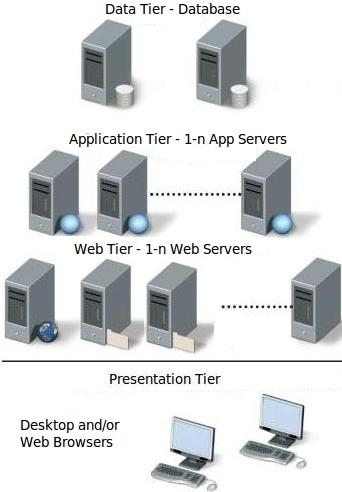
\includegraphics[scale=0.7]{multi-tier-system.png}
	\captionof{figure}{Arquitetura de Aplicação Distribuída (adaptada de \cite{multi-tier-system}).}
	\label{fig:tree-tiers-app}
\end{center}

Segundo \cite{coulouris2007sisdist}, um sistema distribuído traz benefícios como: permitir a heterogeneidade de componentes,
possibilitar a escalabilidade, ser tolerante a falhas, dentre outros.

Neste contexto, \textit{Web Services} (WSs)\nomenclature{WS}{\textit{Web Service}} proveem um \textit{framework} extensível para comunicação de aplicação para aplicação, que utiliza protocolos \textit{Web} existentes e baseados em padrões XML\nomenclature{XML}{\textit{eXtensible Markup Language}} abertos \cite{curbera2002unraveling}. Eles são a maior tecnologia para publicação de serviços na \textit{Web} e têm \replaced{significativa}{significante} adoção em áreas como integração de aplicações, computação distribuída de larga escala e cooperação \textit{business-to-business} (B2B\nomenclature{B2B}{\textit{Business-to-Business}}) \cite{kopecky2008semantic}. Os mesmos são instalados na Camada de Aplicação, como mostrado na Figura \ref{fig:tree-tiers-app}, e proveem um conjunto de padrões para acesso a serviços pela \textit{Internet}, sendo uma tecnologia estabelecida no mercado e cada vez mais adotada por empresas \cite{lausen2007finding}.

\textit{Web Services} permitem o desenvolvimento baseado em componentes, acessíveis por meio da \textit{Internet}. Eles são componentes reutilizáveis, que as aplicações, independentemente da linguagem em que foram implementadas, podem utilizar sem se preocupar em como eles foram desenvolvidos \cite{vilas2007providing}. Desta forma, a construção de aplicações a partir de Web Service segue o processo de desenvolvimento
de \textit{software} conhecido como componentização, como apresentado em \cite{sommerville2011soft}.

Diferentemente de tecnologias como \textit{Common Object Request Broker Architecture} (CORBA)\nomenclature{CORBA}{\textit{Common Object Request Broker Architecture}}, \textit{Distributed Component Object Model} (DCOM)\nomenclature{DCOM}{\textit{Distributed Component Object Model}}, \textit{Component Object Model Plus} (COM+)\nomenclature{COM+}{\textit{Component Object Model Plus}} e 
Java \textit{Remote Method Invocation} (RMI)\nomenclature{RMI}{\textit{Remote Method Invocation}}, WSs usam protocolos \textit{Web} e formatos de dados ubíquos, como HTTP e XML \cite{vilas2007providing}. 

O objetivo dos \textit{Web Services} é alcançar a interoperabilidade entre aplicações, usando padrões \textit{Web}
(\textit{Web standards}). Eles usam um modelo de integração fracamente acoplado para permitir
a integração flexível de sistemas heterogêneos em uma variedade de domínios, 
incluindo \textit{Business-to-Consumer} (\textit{B2C})\nomenclature{B2C}{\textit{Business-to-Consumer}},
\textit{Business-to-Business} (\textit{B2B})
e \textit{Enterprise Application Integration} (\textit{EAI})\nomenclature{EAI}{\textit{Enterprise Application Integration}} \cite{oasis-wsbpel}.


Pela própria natureza distribuída da \textit{Web}, o uso de WSs vem ao encontro da integração entre aplicações heterogêneas, executando em diferentes plataformas, desenvolvidas por diferentes empresas. Cada vez mais empresas disponibilizam serviços, públicos ou privados, para serem utilizados por terceiros, permitindo a interoperabilidade entre diferentes sistemas. Além disto, pelo fato de WSs serem transportados, principalmente, por protocolo HTTP, não sofrem com problemas de portas bloqueadas em \textit{Firewalls} que outras tecnologias, como as mencionadas anteriormente, encontram.
Isto facilita ainda mais a integração entre sistemas hospedados em diferentes redes.

Um \textit{framework} de WSs pode ser dividido em três áreas: protocolos de comunicação,
descrição de serviços e descoberta de serviços \cite{sommerville2011soft}, conforme apresenta 
a Figura \ref{fig:arq-sis-orientados-servicos} e as sub-seções seguintes.

\begin{center}
	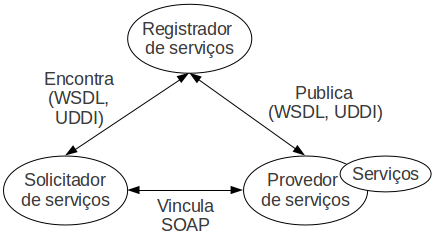
\includegraphics[width=0.7\textwidth]{arq-sis-orientados-servicos.png}
	\captionof{figure}[Arquitetura conceitual de sistemas orientados a serviços]{Arquitetura conceitual de sistemas orientados a serviços (adaptada de \cite{sommerville2011soft}).}
	\label{fig:arq-sis-orientados-servicos}
\end{center}

\subsection{Protocolos de Comunicação}

Dada a natureza distribuída e heterogênea da \textit{Web}, mecanismos de comunicação
devem ser independentes de plataforma, seguros e leves quanto possível.
A linguagem XML é um padrão altamente utilizado para codificação e intercâmbio de dados
entre sistemas, sendo totalmente independente de plataforma. Por esse motivo,
a mesma é utilizada no protocolo de comunicação usado por WSs.

O \textit{Simple Object Access Protocol} (SOAP)\nomenclature{SOAP}{\textit{Simple Object Access Protocol}}, é um protocolo padronizado pelo \textit{World Wide Web Consortium} (W3C),
como protocolo de comunicação para WSs. O SOAP é um protocolo, baseado em XML, para a troca
de mensagens e chamadas de procedimentos remotos (\textit{Remote Procedure Call}, 
RPC\nomenclature{RPC}{\textit{Remote Procedure Call}}). 
No lugar de definir um novo protocolo para empacotar as mensagens, SOAP utiliza protocolos \textit{Web} existentes como HTTP\nomenclature{HTTP}{\textit{HyperText Transfer Protocol}} e SMTP\nomenclature{SMTP}{\textit{Simple Mail Transfer Protocol}}.

Ele é um protocolo leve, adequado para comunicação em um ambiente distribuído e descentralizado \cite{vilas2007providing}.

Uma mensagem SOAP, também denominada "envelope SOAP", é composta por um arquivo XML, contendo um elemento \textit{header} e um \textit{body}.
A Listagem \ref{list:soap-message} mostra a estrutura de um envelope SOAP.

\lstset{caption=Estrutura de um envelope SOAP \cite{curbera2002unraveling}, label=list:soap-message}
\begin{lstlisting}[language=xml]
<SOAP:Envelope 
  xmlns:SOAP="http://schemas.xmlsoap.org/soap/envelope/">
  <SOAP:Header>
      <!-- content of header goes here -->
  </SOAP:Header>

  <SOAP:Body>
      <!-- content of body goes here -->
  </SOAP:Body>
</SOAP:Envelope>
\end{lstlisting}

\subsubsection{Troca de Mensagens SOAP}

Como exemplo para esta seção, vamos utilizar um sistema \textit{Web} de uma companhia aérea, como apresentado em \cite{curbera2002unraveling}.
O sistema disponibiliza um \textit{Web Service} (WS) para a compra de passagens. Uma empresa que vende pacotes turísticos
pode utilizar este WS para integrar o seu sistema com o da companhia aérea,
e assim, fazer todo o processo de registro da passagem dentro do seu próprio sistema.
Desta forma, o sistema da empresa de turismo deve enviar um envelope SOAP
para o WS disponibilizado pela companhia aérea, contendo os dados do cliente
e dados da passagem a ser adquirida, como data/hora, número do voo e do assento 
escolhido pelo cliente. A Listagem \ref{list:http-soap-message} mostra um exemplo
de tal envelope SOAP, empacotado numa mensagem HTTP.

\lstset{caption=Envelope SOAP transportado via HTTP \cite{curbera2002unraveling}, label=list:http-soap-message}
\begin{lstlisting}[language=xml]
POST /travelservice
SOAPAction: "http://www.acme-travel.com/checkin"
Content-Type: text/xml; charset="utf-8"
Content-Length: nnnn

<SOAP:Envelope 
   xmlns:SOAP="http://schemas.xmlsoap.org/soap/envelope/">
   <SOAP:Body>
      <et:eTicket xmlns:et=
         "http://www.acme-travel.com/eticket/schema">
         <et:passengerName first="Joe" last="Smith"/>
         <et:flightInfo airlineName="AA"
              flightNumber="1111"
              departureDate="2002-01-01"
              departureTime="1905"/>
      </et:eTicket>
    </SOAP:Body>
</SOAP:Envelope>
\end{lstlisting}

Observe que o envelope SOAP da Listagem \ref{list:http-soap-message} não possui um \textit{header}.
O mesmo é um elemento opcional e utilizado para prover informações específicas da aplicação,
como credenciais para acesso ao serviço e informações de cobrança, dentre outras\cite{soap-tutorial}.

\subsubsection{Chamadas de Procedimento Remoto Usando SOAP}

Para que SOAP possa usar RPC para chamar procedimentos remotos, é necessário
especificar alguns detalhes para o protocolo RPC, por exemplo:

\begin{itemize}
	\item como valores de tipos são transportados entre  a representação SOAP (XML)
   e a representação da aplicação, e vice-versa (para indicar, por exemplo,
   como deve ser feita a conversão de uma classe Java para XML e vice-versa), e
   \item onde as várias partes do protocolo RPC são transportadas (identificação
   de objeto, nome da operação e parâmetros de entrada e saída).
\end{itemize}

A especificação XML \textit{schema} do W3C \footnote{\url{http://www.w3.org/XML/Schema}} provê uma linguagem padrão
para definir a estrutura do documento e os tipos de dados da estrutura do XML. Isto é,
dado um tipo básico como \textit{integer} ou um tipo complexo como uma \textit{struct}, XML \textit{schema} oferece
uma forma padrão de escrever dados destes tipos em um documento XML. Para habilitar o transporte
de valores tipados, SOAP assume um sistema de tipos baseado em XML \textit{schema}
e define sua codificação em XML. Usando este estilo de codificação pode-se produzir
uma codificação XML para qualquer tipo de dado estruturado.
Parâmetros RPC e retornos são especificados usando esta codificação.

Usando o mesmo WS da companhia aérea, a empresa de turismo
deseja obter informações a respeito de um determinado voo. Assim, seu
sistema pode enviar um envelope SOAP ao WS da companhia aérea.
O envelope da Listagem \ref{list:soap-rpc} mostra uma chamada RPC, encapsulada
dentro de um envelope SOAP. O envelope permite a invocação do método remoto 
\textit{GetFlightInfo}, que recebe dois parâmetros: uma \textit{string} contendo o nome da companhia 
aérea, e um inteiro contendo o número do voo. Tal método retorna um valor estruturado
(uma \textit{struct}) com dois campos: o número do portão de embarque e a situação do voo.

No envelope SOAP, a chamada para \textit{GetFlightInfo} é um elemento XML com atributos
que incluem informações sobre a codificação (note a referência para o XML \textit{schema}). 
Os elementos filhos são os argumentos do método: \textit{airlineName} e \textit{flightNumber}. 
Os tipos são definidos no atributo \textit{type}, onde \textit{xsd} refere-se as definições
de um XML \textit{schema}. Quando o servidor SOAP recebe o envelope, ele converte os valores
\textit{string}, dos atributos \textit{airlineName} e \textit{flightNumber}, para seus
respectivos tipos \textit{string} e inteiro, chamando o método \textit{GetFlightInfo}
passando estes valores.

\lstset{caption=Chamada SOAP RPC empacotada em HTTP \cite{curbera2002unraveling}, label=list:soap-rpc}
\begin{lstlisting}[language=xml]
POST /travelservice
SOAPAction: "http://www.acme-travel.com/flightinfo"
Content-Type: text/xml; charset="utf-8"
Content-Length: nnnn

<SOAP:Envelope 
  xmlns:SOAP="http://schemas.xmlsoap.org/soap/envelope/">
  <SOAP:Body>
    <m:GetFlightInfo
      xmlns:m="http://www.acme-travel.com/flightinfo"
      SOAP:encodingStyle="http://schemas.xmlsoap.org/soap/encoding/"
      xmlns:xsd="http://www.w3.org/2001/XMLSchema"
      xmlns:xsi="http://www.w3.org/2001/XMLSchema-instance">
         <airlineName xsi:type="xsd:string">UL</airlineName>
         <flightNumber xsi:type="xsd:int">506</flightNumber>
    </m:GetFlightInfo>
  </SOAP:Body>
</SOAP:Envelope>
\end{lstlisting}

A Listagem \ref{list:soap-response} mostra a resposta à requisição SOAP enviada
anteriormente. Neste caso, a resposta contém um valor estruturado, com
os campos \textit{gate} (número do portão de embarque) e \textit{status} (situação do voo).

Implementações de SOAP existem para diversas linguagens, como C/C++, Java, Perl e Lua\footnote{Uma implementação
do protocolo SOAP foi feita para uso em aplicações de TV digital desenvolvidas em NCL e Lua, e será apresentada no Capítulo \ref{cap:ncluasoap}.}, que automaticamente geram e processam mensagens SOAP.
Assumindo que as mensagens estão em conformidade com as especificações do protocolo SOAP,
elas podem ser trocadas por serviços implementados em diferentes linguagens e plataformas,
permitindo uma total interoperabilidade entre sistemas heterogêneos, algo que não é sempre
verdade para sistemas que utilizam a arquitetura CORBA, que possui objetivos semelhantes ao SOAP.

\lstset{caption=Resposta de requisição SOAP empacotada em HTTP \cite{curbera2002unraveling}, label=list:soap-response}
\begin{lstlisting}[language=xml]
HTTP/1.1 200 OK
Content-Type: text/xml; charset="utf-8"
Content-Length: nnnn

<SOAP:Envelope 
  xmlns:SOAP="http://schemas.xmlsoap.org/soap/envelope/">
  <SOAP:Body>
    <m:GetFlightInfoResponse 
      xmlns:m="http://www.acme-travel.com/flightinfo"
      SOAP:encodingStyle="http://schemas.xmlsoap.org/soap/encoding/"
      xmlns:xsd="http://www.w3.org/2001/XMLSchema"
      xmlns:xsi="http://www.w3.org/2001/XMLSchema-instance">
         <flightInfo>
           <gate xsi:type="xsd:int">10</gate>
           <status xsi:type="xsd:string">ON TIME</status>
         </flightInfo>
     </m:GetFlightInfoResponse>
   </SOAP:Body>
</SOAP:Envelope>
\end{lstlisting}

\subsection{Descrição de Serviços}

O protocolo SOAP define uma linguagem padrão para uso de WSs,
mas ele não informa quais mensagens devem ser trocadas para 
que tenhamos sucesso no uso de um determinado serviço.
Para isto, existe a \textit{Web Service Description Language} (WSDL)\nomenclature{WSDL}{\textit{Web Service Description Language}}, 
uma linguagem também baseada em XML. Um documento WSDL descreve
a interface de um WS, permitindo que as aplicações
que consumirão o serviço disponibilizado, saibam quais informações
devem incluir dentro de um envelope SOAP. Desta forma, podem chamar
um determinado procedimento remoto disponibilizado pelo WS.
O WSDL descreve um WS como uma coleção de \textit{end points}
que podem trocar certas mensagens \cite{curbera2002unraveling}. Um \textit{end point} é um
elemento no WSDL que define a ligação entre a definição de um 
determinado serviço e o seu endereço de rede, permitindo o acesso
ao mesmo.

As mensagens SOAP anteriormente mostradas não poderiam ter sido
construídas se não conhecêssemos o documento WSDL que descreve
o serviço que desejamos utilizar. Informações
como o nome do método a ser acessado e o nome e tipos dos parâmetros
de entrada e saída foram obtidos a partir do WSDL do serviço \cite{curbera2002unraveling}.

Um serviço completo de descrição WSDL provê dois pedaços de informação:
uma descrição do serviço em nível de aplicação, ou interface abstrata, e 
detalhes específicos dependentes do protocolo, que os usuários
devem seguir para acessar o serviço em \textit{end points} concretos \cite{curbera2002unraveling}.

\subsubsection{Descrição de um \textit{Web Service}}

Um documento WSDL define uma descrição abstrata de um serviço, em termos
de troca de mensagens em uma interação com o mesmo. Existem três principais
componentes desta interface abstrata: o vocabulário, a mensagem e a interação. 
Acordo para uso de um determinado vocabulário é a fundação para qualquer tipo
de comunicação. Um WSDL usa sistemas de tipos externos para prover definição
de tipos de dados para troca de informações. Embora o WSDL possa suportar
qualquer sistema de tipos, a maioria dos serviços usa o XML \textit{Schema Definition} (XSD)\nomenclature{XSD}{\textit{XML Schema Definition}}.
Na Listagem \ref{list:wsdl-description}, podemos ver o uso de dois tipos 
de dados definidos no XSD (\textit{int} e \textit{string}), e dois tipos de dados definidos
em um \textit{schema} externo (\textit{FlightInfoType} e \textit{Ticket}).
O WSDL pode importar tais definições XSD externas usando um elemento 
\textit{import}, especificando sua localização \cite{curbera2002unraveling}.

O WSDL define elementos \textit{message} contendo partes, cada qual descrita
por tipos XSD ou elementos de um vocabulário pré-definido.
Cada \textit{message} provê uma definição de dados tipados e abstratos
enviados e recebidos pelos serviços. Uma mensagem pode ser de entrada (\textit{input}),
definindo o tipo do(s) parâmetro(s) que uma determinada função deve receber; 
ou de saída (\textit{output}), indicando o(s) tipo(s) de valor(es) a ser(em) retornado(s)
pela função, como pode ser visto na Listagem \ref{list:wsdl-description} \cite{curbera2002unraveling}.

Os elementos \textit{portType} e \textit{operation} combinam mensagens para definir
iterações. Cada \textit{operation} representa um padrão de troca de mensagens
suportado pelo WS. Cada \textit{operation} é uma combinação de mensagens
rotuladas como \textit{input} (entrada), \textit{output} (saída) ou \textit{fault} (falha),
para indicar o papel de cada mensagem em uma iteração \cite{curbera2002unraveling}.

Um \textit{portType} é uma coleção de operações que são coletivamente suportadas
por um \textit{end point} (\textit{port}). No exemplo da Listagem \ref{list:wsdl-description},
\textit{AirportServicePortType} descreve duas operações: uma única operação
no estilo \textit{request-response}, \textit{GetFlightInfo}, que espera
uma mensagem \textit{GetFlightInfoInput} como entrada e retorna
uma mensagem \textit{GetFlightInfoOutput} como resposta; e uma operação
uni direcional, \textit{CheckIn}, que apenas recebe uma mensagem \textit{CheckInInput}
como entrada \cite{curbera2002unraveling}.

\lstset{caption=Fragmento de uma descrição de WSDL \cite{curbera2002unraveling}, label=list:wsdl-description}
\begin{lstlisting}[language=xml]
<message name="GetFlightInfoInput">
  <part name="airlineName" type="xsd:string"/>
  <part name="flightNumber" type="xsd:int"/>
</message>

<message name="GetFlightInfoOutput">
  <part name="flightInfo" type="fixsd:FlightInfoType"/>
</message>

<message name="CheckInInput">
  <part name="body" element="eticketxsd:Ticket"/>
</message>

<portType name="AirportServicePortType">
  <operation name="GetFlightInfo">
    <input message="tns:GetFlightInfoInput"/>                   
    <output message="tns:GetFlightInfoOutput"/>
  </operation>
  <operation name="CheckIn">
    <input message="tns:CheckInInput"/>
</operation>
</portType>
\end{lstlisting}

\subsubsection{Informações de \textit{Binding}}

A especificação do WSDL apresenta três tipos de informações sobre
o serviço\cite{sommerville2011soft}:

\begin{itemize}
	\item quais operações o serviço suporta (chamado de interface);
  \item como mapear as interfaces abstratas para um conjunto de protocolos concretos (\textit{binding}), e
  \item onde está a implementação dos métodos suportados pelo serviço (o endereço de rede).
\end{itemize}


Por meio do \textit{binding} temos a resposta para o "como",
incluindo o protocolo de comunicação e especificação de formato de dados
para um completo elemento \textit{portType}. Sucintamente, o elemento \textit{binding}
diz como dada interação ocorre sobre o protocolo especificado. A Listagem \ref{list:wsdl-binding}
mostra um fragmento para o exemplo citado. O \textit{binding} descreve como usar SOAP
para acessar o serviço \textit{travelservice}. Em particular, o documento WSDL mostra que:

\begin{itemize}
	\item \textit{GetFlightInfo} usará interações em estilo SOAP-RPC,
  em que todas as trocas de mensagens usam codificação padrão SOAP, e
  \item \textit{CheckIn} é uma interação de mensagem pura (chamada de orientada a documento
  em termos de WSDL), em que o corpo do envelope SOAP contém a mensagem codificada,
  sem nenhuma codificação de tipo adicional; isto é, ele usa XSD para literalmente descrever
  o XML transmitido.
\end{itemize}

O restante do documento descreve o "onde", para ligar a interface abstrata, protocolo
e detalhes de \textit{marshalling}\footnote{Processo de organizar dados em computador, de forma padronizada,
para permitir que diferentes aplicações possam utilizar tais dados, garantindo
a interoperabilidade.}, promovendo a ligação (\textit{binding}) desses elementos para permitir
o acesso aos métodos do serviço. Um elemento \textit{port} descreve um único \textit{end point}
como uma combinação de um \textit{binding} e um endereço de rede. Consequentemente, um elemento
\textit{service} pode agrupar um conjunto de \textit{ports} relacionados.

\lstset{caption=Informações concretas de ligação em um WSDL \cite{curbera2002unraveling}, label=list:wsdl-binding}
\begin{lstlisting}[language=xml]
<binding name="AirportServiceSoapBinding"
  type="tns:AirportServicePortType">
  <soap:binding 
     transport="http://schemas.xmlsoap.org/soap/http"/>
  <operation name="GetFlightInfo">
    <soap:operation style="rpc"
          soapAction="http://acme-travel/flightinfo"/>
    <input>
      <soap:body use="encoded"
          namespace="http://acme-travel.com/flightinfo"
          encodingStyle=
           "http://schemas.xmlsoap.org/soap/encoding/"/>
    </input>
    <output>
      <soap:body use="encoded"
          namespace="http://acme-travel.com/flightinfo"
          encodingStyle=
           "http://schemas.xmlsoap.org/soap/encoding/"/>
    </output>
  </operation>

  <operation name="CheckIn">
    <soap:operation style="document"
          soapAction="http://acme-travel.com/checkin"/>
    <input>
      <soap:body use="literal"/>
    </input>
  </operation>
</binding>

<service name="travelservice">
  <port name="travelservicePort"
     binding="tns:AirportServiceSoapBinding">
  <soap:address 
     location="http://acmetravel.com/travelservice"/>
  </port>
</service>
\end{lstlisting}

A Figura \ref{fig:wsdl-organization} mostra como a especificação do WSDL é organizada.
A seção \textit{Introdução} do WSDL contém a declaração dos \textit{Namespaces} XML contendo as definições
de tipos padrões usados pelo \textit{Web Service}. A seção \textit{Interface Abstrata}
apresenta os tipos definidos pelo \textit{Web Service}, as declarações de interfaces (os \textit{portTypes})
e as mensagens suportadas (como mensagens com os parâmetros de entrada a serem enviadas a um método no \textit{Web Service}
e as mensagens de saída com o retorno do método).
A seção \textit{Implementação Concreta} contém as informações de \textit{binding} (como o protocolo a
ser utilizado na troca de mensagens) e os \textit{end points} (as interfaces
concretas para realização da vinculação da aplicação cliente com o endereço de rede do \textit{Web Service}.

\begin{center}
	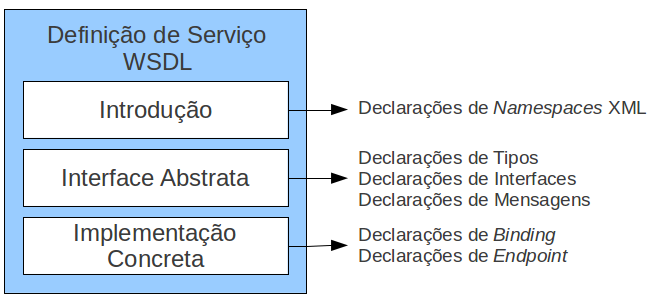
\includegraphics[width=0.80\textwidth]{wsdl-organization.png}
	\captionof{figure}[Organização da Especificação do WSDL]{\added{Organização da Especificação do WSDL\cite{sommerville2011soft}.}}
	\label{fig:wsdl-organization}
\end{center}



\subsubsection{Usando o WSDL}

Para usuários e desenvolvedores, o WSDL provê uma descrição formal das interações cliente/servidor.
Desenvolvedores podem usar o documento WSDL como entrada para uma aplicação que gere 
funções \textit{proxy}\footnote{Tais funções \textit{proxy} são escritas ou geradas
na linguagem utilizada pela aplicação cliente (que consome o \textit{Web Service}). Elas possuem
a mesma assinatura dos métodos remotos, tornando transparente para o cliente a chamada
aos métodos no WS. São responsáveis por gerar o envelope SOAP para enviar ao
servidor onde o WS é hospedado.},
utilizadas no cliente, para acesso aos métodos do WS. Tais funções \textit{proxy}
também podem ser geradas dinamicamente, em tempo de execução, por rotinas implementadas
no cliente que interpretam o WSDL e geram as chamadas SOAP necessárias.
Em ambos os casos, as funções \textit{proxy} têm a finalidade de esconder do cliente toda a complexidade
envolvida no processo de chamada dos métodos remotos.

\subsection{Descoberta de Serviços com UDDI} \label{sec:uddi}

As especificações do \textit{Universal Description, Discovery and Integration} (UDDI)\nomenclature{UDDI}{\textit{Universal Description, Discovery and Integration}} oferecem aos usuários uma forma sistemática e unificada para encontrar provedores
de serviços através de um registro centralizado de serviços, que é, grosseiramente,
equivalente a uma "lista telefônica" \textit{online} de WSs \cite{curbera2002unraveling}.
O \textit{UDDI Business Registry} (UBR)\nomenclature{UBR}{\textit{UDDI Business Registry}}, acessível por meio de um \textit{browser}, foi
disponibilizado pouco tempo após a especificação se tornar pública, no entanto, o mesmo foi descontinuado
em 2005\footnote{\url{http://uddi.microsoft.com/about/FAQshutdown.htm}} \cite{treiber2007active}.

Segundo \cite{sommerville2011soft}, o padrão UDDI não foi amplamente adotado.
UDDI provê dois tipos básicos de especificação que definem a estrutura
e operação do registro de serviços \cite{curbera2002unraveling}:

\begin{itemize}
	\item uma definição da informação para prover sobre cada serviço, e como codificá-la; e
  \item uma API\nomenclature{API}{\textit{Application Programming Interface}} de busca e atualização para o registro, que descreve como esta informação
  pode ser acessada e atualizada.
\end{itemize}

O acesso ao registro é realizado usando uma API SOAP para busca e atualização. 

\begin{comment}
\subsubsection{Estrutura do UDDI}

O UDDI codifica três tipos de informações sobre \textit{Web Services}:

\begin{itemize}
	\item informações de \textbf{páginas brancas} incluem nome e detalhes de contato;
  \item informações de \textbf{páginas amarelas} proveem uma categorização baseada em tipos
  de negócio e serviço; e
  \item informações de \textbf{páginas verdes} incluem dados técnicos sobre o serviço.
\end{itemize}

O registro UDDI é organizado ao redor de duas entidades fundamentais que descrevem negócios e os serviços que eles proveem. O elemento \textit{businessEntity} (entidade de negócio), apresentado na Listagem \ref{list:uddi-businessEntity}, provê informações padrões de "páginas brancas", incluindo identificadores (como CPF/CNPJ), informações de contato e uma descrição simples. Cada entidade de negócio deve incluir deve incluir um ou mais elementos \textit{businessServices} (serviço de negócio), mostrado na Listagem \ref{list:uddi-businessService}, que representam os serviços que ele provê. Ambas elementos de negócio e serviço podem especificar um elemento \textit{categoryBag} para categorizar o negócio ou serviço (que será discutido adiante).

\lstset{caption=Estrutura simplificada do \textit{businessEntity} de um serviço no UDDI \cite{curbera2002unraveling}, label=list:uddi-businessEntity}
\begin{lstlisting}[language=xml]
<businessEntity businessKey=
       "A687FG00-56NM-EFT1-3456-098765432124">
 <name>Acme Travel Incorporated</name>
 <description xml:lang="en">
   Acme is a world leader in online travel services
 </description>
 <contacts>
   <contact useType="US general">
     <personName>Acme Inc.</personName>
     <phone>1 800 CALL ACME</phone>
     <email useType="">acme@acme-travel.com</email>
     <address>
       <addressLine>Acme</addressLine>
       <addressLine>12 Maple Avenue</addressLine>
       <addressLine>Springfield, CT 06785</addressLine>
     </address>
   </contact>
 </contacts>
 <businessServices> ...
 </businessServices>
 <identifierBag> ...
 </identifierBag>
 <categoryBag> ...
   <keyedReference tModelKey=
         "UUID:DB77450D-9FA8-45D4-A7BC-04411D14E384"
         keyName="Electronic check-in"
         keyValue="84121801"/>
 </categoryBag>
</businessEntity>
\end{lstlisting}

As Listagens \ref{list:uddi-businessEntity} e \ref{list:uddi-businessService} mostram um importante aspecto do projeto de UDDI: chaves únicas identificam cada entidade de dados - negócios, serviços e tudo mais - que podem referenciar umas as outras. Estas chaves são \textit{strings} hexadecimais geradas quando a entidade (neste caso, o negócio) é registrada. As chaves são identificadores universalmente únicos (\textit{Universally Unique Identifiers}, UUIDs). Por exemplo, o atributo \textit{businessKey} (chave de negócio) identifica um negócio unicamentee um atributo \textit{serviceKey} (chave de serviço) identifica unicamente um serviço. Um serviço também referencia seu host pela sua \textit{businessKey}. Em adição a informações inteligíveis como descrição, nome e categorização, a entidade \textit{service} contém uma lista de \textit{bindingTemplates}, que codificam informações técnicas de acesso ao serviço. Cada \textit{bindingTemplate} representa um ponto de acesso ao serviço, indicando que o serviço pode ser acessado de diferentes \textit{end points}.

\lstset{caption=Estrutura simplificada do \textit{businessService} de um serviço no UDDI \cite{curbera2002unraveling}, label=list:uddi-businessService}
\begin{lstlisting}[language=xml]
<businessService serviceKey=
      "894B5100-3AAF-11D5-80DC-002035229C64"
    businessKey=
      "D2033110-3AAF-11D5-80DC-002035229C64">
  <name>ElectronicTravelService</name>
  <description xml:lang="en">Electronic Travel Service</description>
  <bindingTemplates>
    <bindingTemplate bindingKey=
          "6D665B10-3AAF-11D5-80DC-002035229C64"
        serviceKey=
          "89470B40-3AAF-11D5-80DC-002035229C64">
      <description>
        SOAP-based e-checkin and flight info
      </description>
      <accesssPoint URLType="http">
        http://www.acme-travel.com/travelservice
      </accessPoint>
      <tModelInstanceDetails>
        <tModelInstanceInfo tModelKey=
          "D2033110-3BGF-1KJH-234C-09873909802">
        ...
        </tModelInstanceInfo>
      </tModelInstanceDetails>
    </bindingTemplate>
  </bindingTemplates>
  <categoryBag> ...
  </categoryBag>
</businessService>
\end{lstlisting}

\subsubsection{Descrição Técnica e tModels}
...

\subsubsection{Categorização}

Localizar particulares tipos de negócios e serviços eficientemente depende da nossa habilidade de qualificar as entradas de negócios e serviços no diretório, de acordo com um esquema de categorização ou taxonomia, usando informações como localização geográfica, tipo de indústria ou produto, para caracterizar o serviço.

Para identificar sistemas de taxonomia, cada sistema de classificação é registrado com um \textit{tModel} no registro UDDI. Informações taxonômicas são então codificadas em pares de nome-valor, qualificados por uma referência a uma chave de um \textit{tModel}, que identifica a qual taxonomia cada par pertence. Três taxonomias padrões são citadas pelo UDDI e pré-registradas no UBR:

\begin{itemize}
	\item uma classificação de indústria, obedecendo à taxonomia do \textit{North American Industry Classification System},NAICS (Sistema de Classificação Industrial Norte Americano)\nomenclature{NAICS}{\textit{North American Industry Classification System}};
  \item uma classificação de produtos e serviços obedecendo à taxonomia do \textit{Universal Standard Products and Services Code System} (USPSCS) (Padrão Universal de Sistema de Código de Produtos e Serviços)\nomenclature{USPSCS}{\textit{Universal Standard Products and Services Code System}}; e
  \item um sistema de categorização geográfica obedecendo à taxonomia do \textit{International Organization for Standardization Geographic} (ISO 3166\footnote{Um padrão de identificação de países, que possui tanto códigos alfabéticos no formato de 2 e 3 letras, quanto códigos numéricos de 3 dígitos. Os códigos para o Brasil, por exemplo, podem ser BR, BRA ou 076.}).\nomenclature{ISO}{\textit{International Organization for Standardization}}
\end{itemize}

Usando categorização, podemos pesquisar no diretório UDDI por tipos de serviços específicos. Um vez encontrado o serviço, podemos obter sua descrição WSDL para saber como utilizá-lo.
\end{comment}

\subsection{\textit{Web Services} REST}

Como visto anteriormente, SOAP é o padrão W3C para \textit{Web Services}, amplamente utilizado
na integração de aplicações heterogêneas. No entanto, existe uma outra vertente para construção de \textit{Web Services}
denominada REST. O REST é o acrônimo para \textit{Representational State Transfer}\nomenclature{REST}{\textit{Representational State Transfer}}. 
Ele é um estilo arquitetural para construção de aplicações distribuídas que também permite a integração de aplicações heterogêneas,
mas não é um padrão W3C.

O estilo REST foi apresentado pela primeira vez no trabalho de dissertação de Roy Fielding\cite{fielding2000architectural},
sendo baseado em padrões \textit{Web} como HTTP e URL. Ele consiste em prover serviços \textit{Web}
a partir de um recurso \textit{Web} acessível por meio de uma URL\nomenclature{URL}{\textit{Uniform Resource Locator}}. 
A interação com tal serviço é feita por meio de uso dos métodos HTTP como \textit{GET}, \textit{POST} e \textit{DELETE} para passagem de parâmetros ao serviço.
Tal estilo é bastante simplificado em relação ao SOAP, pois todos os dados a serem passados ao serviço
vão diretamente na URL do mesmo, por meio de uma requisição HTTP. Desta forma, o tamanho de uma requisição REST
é bastante reduzido em relação ao SOAP.

REST não define um padrão de formato das mensagens de resposta, no entanto, pode-se perfeitamente utilizar
XML para isto. Atualmente outros padrões de formato de dados são bastante utilizados como o \textit{JavaScript Object Notation} (JSON)\nomenclature{JSON}{\textit{JavaScript Object Notation}}. Desta forma, pode-se utilizar qualquer padrão que se desejar, como por exemplo,
o formato de dados definido pela linguagem Lua, sendo bastante útil em aplicações para o Sistema Brasileiro de TV Digital, desenvolvidas em tal  linguagem, por utilizar um formato nativo da mesma.

O estilo REST atualmente se tornou um padrão de fato e é amplamente utilizado para integração
de serviços \textit{Web} com aplicações de diferentes tipos, como é o caso dos serviços disponibilizados
pelo \textit{microblog Twitter}. Este permite que desenvolvedores construam aplicações 
nas mais diferentes plataformas (\textit{Web, desktop, mobile}) que se integrem
com o serviço de \textit{microblog}.

O REST também segue a arquitetura cliente/servidor usada no protocolo SOAP. 
Segundo \cite{welling2006integration}, o estilo é denominado REST (em português, Transferência de Estado Representacional), pois o cliente obtém
uma representação de um recurso através de uma URL, o que faz com que a aplicação cliente
entre em um determinado estado. O cliente pode selecionar um link que foi incluído no primeiro recurso para,
por exemplo, obter informações detalhadas. Como o link direciona para outro recurso, a aplicação cliente
obtém uma nova representação de um recurso e entra em um novo estado.

Como citado, a grande vantagem do REST é sua simplicidade, no entanto, 
por não haver um padrão de passagem de parâmetros e formato de dados
para a respostas das requisições, tal estilo pode não ser adequado para 
a construção de aplicações seguindo o padrão de arquitetura orientada
a serviços, onde uma aplicação pode utilizar serviços de diferentes provedores.
Usando REST, cada provedor de serviços pode definir sua forma de passar os parâmetros
e o formato de dados da mensagem de retorno, assim a aplicação que integra com todos
os provedores precisará implementar diversos formatos de entrada e saída de dados.
Com o SOAP isto não ocorre, pois todos os provedores seguem um padrão bem definido
e a aplicação cliente implementa apenas tal padrão.

\subsection{Arquitetura Orientada a Serviços}

Segundo \cite{sommerville2011soft}, uma arquitetura orientada a serviços (\textit{Service Oriented Architecture} - SOA)
é uma forma de desenvolvimento de sistemas distribuídos onde os componentes de tal sistema são serviços \textit{stand-alone} (autônomos),
executando em computadores geograficamente distribuídos. Em tal arquitetura, ainda segundo \cite{sommerville2011soft}, 
usar \textit{Web Services} é uma forma de as organizações tornarem suas informações acessíveis. Com isto, é possível
haver a integração entre empresas, mesmo que por meio de sistemas heterogênos completamente diferentes.

 %input no lugar de include evita a quebra de linha inserida por este

%Descoberta de Serviços
%input no lugar de include evita a quebra de linha inserida por este
%\section{Propostas para Descoberta de Serviços} \label{sec:propostas-descoberta-ws}

Devido ao encerramento dos repositórios UDDI públicos, suportados pela W3C,  como apresentado na Seção \ref{sec:uddi} e mencionado em \cite{lausen2007finding} \cite{treiber2007active}, surgem novas propostas para descoberta de serviços, como \cite{lausen2007finding} \cite{wu2008novel} \cite{wu2009new} \cite{al2008toward} \cite{borges2007arquitetura}. Algumas delas serão apresentadas nas sub-seções seguintes.

\subsection{\textit{A Novel Interoperable Model of Distributed UDDI} \cite{wu2008novel}} \label{sec:novel-model-uddi}

Segundo \cite{wu2008novel}, a maioria dos modelos de UDDI são centralizados, o que pode acarretar perda de performance caso existam muitos serviços para serem registrados ou pesquisados. Tal arquitetura centralizado não possui tolerância a falhas e não permite balanceamento de carga. Outro problema de tais modelos é a falta de detecção ativa de mudanças em \textit{Web Services} e captura de falhas, impedindo que seja informado aos clientes que um determinado serviço não está funcional.

Em \cite{wu2008novel} é apresentada uma arquitetura distribuída para repositórios UDDI, sendo composta de servidores raiz, super servidores de domínio e servidores normais, descritos a seguir. 

Os servidores raiz são um grupo de servidores, semelhantes a servidores raízes DNS, podendo ser um ou mais. Eles não realizam busca e publicação de serviços, apenas registram informações dos super servidores de domínio e proveem a função de registro e busca por este tipo de servidor para compor o repositório UDDI.

Os super servidores de domínio são responsáveis pelo gerenciamento dos servidores normais mais próximos, e proveem registro e busca de serviços, além de poderem obter informações relacionadas de outros super servidores de domínio, a partir dos servidores raiz, para obter mais informações de serviços.

Os servidores normais são usados para permitir aos usuários, publicarem e buscarem por informações de serviços. Eles enviam requisições de busca aos super servidores de domínio se não existir nenhum serviço adequado. A Figura \ref{fig:distributed-uddi} apresenta a arquitetura da proposta.

\begin{center}
	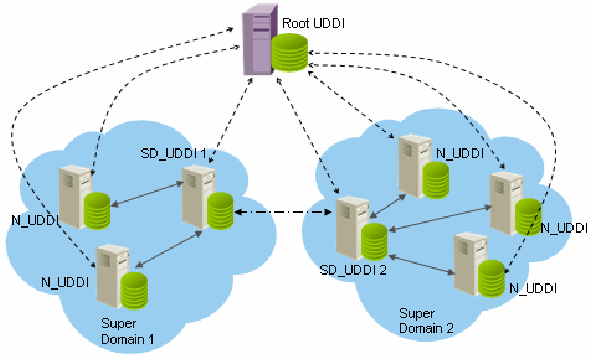
\includegraphics[scale=0.6]{images/a-novel-interoperable-model-uddi.png}
	\captionof{figure}{Arquitetura Distribuída de Repositório UDDI \cite{wu2008novel}}
	\label{fig:distributed-uddi}
\end{center}

Alguns dos objetivos desta arquitetura são: permitir registrar informações sobre os serviços que se tornaram inativos e reduzir o tempo de resposta na busca de serviços. Os autores declarem ter atingido tais objetivos.



%\subsection{\textit{Active Web Service Registries} \cite{treiber2007active}} \label{sec:active-ws-reg}

A proposta para descoberta de serviços, apresentada em \cite{treiber2007active}, consiste em uma arquitetura distribuída para repositórios de descoberta de serviços, denominada \textit{Active Web Service Registry} (AWSR)\nomenclature{AWSR}{\textit{Active Web Service Registry}}. A arquitetura utiliza o formato \textit{Atom} de sindicalização de notícias para registrar os serviços diponibilizados por um provedor. Desta forma, a publicação dos serviços pode ser feita utilizando um dos muitos softwares para geração de \textit{feeds} RSS e \textit{Atom}, disponíveis no mercado.

É utilizado o modelo de dados \textit{Atom} para armazenar informações relevantes sobre os serviços, como descrições textuais, exemplos de utilização e o endereço do WSDL que descreve o serviço. Desta forma, os clientes podem receber notificações sobre atualizações e novos serviços, utilizando clientes RSS/\textit{Atom} padrões\footnote{Existem muitos softwares que suportam o formato RSS/\textit{Atom}, como clientes de \textit{e-mail}, navegadores \textit{Web}, \textit{widgets} e softwares específicos.}.

Na arquitetura proposta, cada provedor de serviços é responsável por gerar seu \textit{feed Atom}, utilizando algum software padrão, para publicar atualizações e novos serviços, criando um ambiente descentralizado, diferente dos modelos tradicionais de UDDI. Desta forma, cada provedor é um \textit{Active Web Service Registry}. O processo de descoberta é feito pelo cliente, que assina este \textit{feed}, utilizando algum software padrão.

Para que o cliente possa descobrir os \textit{Active Web Service Registry}, existem duas propostas citadas em \cite{treiber2007active}: 
\begin{itemize}
	\item adicionar uma tag \textit{link} dentro do cabeçalho de uma página Web, que, quando acessada pela maioria dos navegadores Web atuais, avisará o usuário que aquela página possui um \textit{feed} e solicitará a assinatura do mesmo; e
  \item usar sites indexadores, similares a agregadores de notícias RSS/\textit{Atom} (como o \textit{FeedBurner}\footnote{\url{http://feedburner.google.com}}), para publicar os \textit{feeds} AWSR.
\end{itemize}

A arquitetura é interessante, pois utiliza um modelo de dados \textit{Atom}, amplamente difundido, permitindo a utilização de ferramentas existentes no mercado, tanto para gerar \textit{feeds} para registrar os serviços, quanto para manter os usuários a par de atualizações e novos serviços disponibilizados. Além de criar um ambiente distribuído para a publicação de serviços.


%\subsection{\textit{A New Description Model of Web Service} \cite{wu2009new}} \label{sec:ws-description-model}

Como descrever e descobrir serviços é um problema chave de integração de aplicações baseadas em \textit{Web Services}. Em \cite{wu2009new} é desenvolvido um modelo para descrição semântica de \textit{Web Services}, utilizando padrões como WSDL e OWL-S\nomenclature{OWL-S}{\textit{Semantic Markup for Web Services}} (\textit{Semantic Markup for Web Services}), estendendo a arquitetura de UDDI para procurar e combinar \textit{Web Services} mais fácil e acuradamente.

As descrições podem ser classificadas em descrição de objetos, de interface, de realização e descrições não-funcionais (como parâmetros de QoS\nomenclature{QoS}{\textit{Quality of Service}}).

O principal método para descrever \textit{Web Services} é a descrição baseada em WSDL, que é usada para descrever o formato da mensagem, tipos de dados, operações, \textit{binding} e outros. No entanto, WSDL é usado para descrever informações básicas de \textit{Web Services}, ele não possui recursos para prover descrições semânticas do serviço.

Para prover descrições semânticas, a proposta de \cite{wu2009new} introduz o uso de OWL-S, um tipo de ontologia de \textit{Web Service}, definida com uso da linguagem OWL\nomenclature{OWL}{\textit{Web Ontology Language}}, a \textit{Web Ontology Language}. A OWL-S provê um conjunto de linguagens padrões para provedores analisarem e descreverem a performance e atributos de \textit{Web Services}, por meio de programas de computador. Assim, \textit{Web Services} podem ser localizados, associados, combinados e monitorados automaticamente. A OWL-S define três principais aspectos de informações semânticas: perfil, modelo e bases de serviço. Perfil de serviço descreve o que o \textit{Web Service} faz, incluindo informações básicas. Modelo de serviço descreve como o \textit{Web Service} opera, e bases de serviço descrevem os detalhes de acesso ao \textit{Web Service}, incluindo: protocolo de rede, formato de mensagem e outros detalhes. Perfil de serviços OWL-S proveem descrição semântica de funcionalidades do serviço, incluindo entrada e saída de dados. Perfil de serviço também atribui parâmetros para qualidade de serviço, tais como garantia de qualidade, \textit{rank} de qualidade e tudo mais, mas não provê definições detalhadas de atributos. Portanto, a proposta de \cite{wu2009new} inclue um modelo detalhado de QoS para prover medidas concretas de qualidade de serviço.

Métodos existentes de descrição de \textit{Web Services} têm dois aspectos de desvantagem: devido à insuficiência de informações semânticas e à dependência de associação de palavras-chave, a acurácia de localização de \textit{Web Services} é baixa. Por outro lado, isto afeta a qualidade de serviço devido a falta de descrições de QoS.



%\subsection{\textit{Finding Web Services} \cite{lausen2007finding}} \label{sec:finding-ws}

Segundo \cite{lausen2007finding}, um documento WSDL provê meios para descrever as propriedades da interface técnica como um documento XML, todavia, não provê suporte para todas as tarefas durante o ciclo de vida de um \textit{Web Service} como: publicação, descoberta, determinação dos detalhes da sequência de invocação, segurança, monitoramente, etc. Atualmente estes detalhes são tratados por desenvolvedores e engenheiros de software.

Quanto à descoberta de serviços, existem várias propostas na literatura de como estender o WSDL para adicionar detalhes semânticos, como a proposta em \cite{wu2009new}, apresentada na Seção \ref{sec:ws-description-model}.
Em \cite{lausen2007finding} é apresentada uma proposta de processo completamente automatizado para descoberta de serviços, onde as informações disponíveis para o serviço são obtidas, integradas em um modelo para permitir a descoberta em um conjunto atualizado de serviços. Neste modelo, descrições do serviço são criadas, principalmente, por processos de análise automáticos e pelo \textit{feedback} da comunidade, no lugar de usar conhecimento de engenheiros de software.

Segundo \cite{lausen2007finding}, baseado na origem de descoberta de serviços e em trabalhos anteriores, as três maiores propostas para descobrir \textit{Web Services} públicos são apresentadas a seguir.

\begin{itemize}
	\item UDDI como repositórios centralizados padrões, que possuem uma base de registro de \textit{Web Services};
  \item Diretórios de serviços que descobrem serviços usando \textit{crawlers}\nomenclature{Crawler}{Programa de computador, também conhecido como spider ou bot, utilizado para varrer a Web e permitir a catalogação das páginas existentes, cujo resultado é utilizado por motores de busca como \textit{Google} e \textit{Yahoo}.} específicos ou registro manual de serviços, oferecendo uma interface Web para a realização de buscas;
  \item Motores de busca padrões que são capazes de restringir a busca de forma a obter descrições WSDL. Embora isto não garante que serão encontrados serviços, isto possivelmente provê a maior cobertura.
\end{itemize}

A escolha de uma das propostas pode ser feita baseada, segundo \cite{lausen2007finding}, em dois aspectos: o número de serviços a encontrar e a qualidade e quantidade de informações associadas a eles, como explicado a seguir.

\begin{itemize}
	\item Número de Serviços: no caso do UDDI, os repositórios públicos começaram a ser desligados no início de 2006, logo, não foi possível realizar uma análise do serviço, no entanto, trabalhos anteriores reportaram que apenas um terço dos 1200 serviços registrados continham referências para arquivos WSDL válidos. 
A Tabela \ref{tab:ws-find-portals} mostra o número de \textit{Web Services} encontrados em diferentes portais Web e motores de busca. A segunda coluna
indica se o portal informa sobre a situação do serviço (se está ativo ou não),
a terceira mostra se o portal categoriza os serviços registrados,
a quarta indica o total de \textit{Web Services} registrados, e a última mostra o total de serviços ativos.
Para determinar o número de serviços disponíveis, via motores de busca como \textit{Google} e \textit{Yahoo}, foram detectados dois problemas: a inexistência de meios de obter todos os resultados\footnote{Segundo \cite{lausen2007finding}, \textit{Google} e \textit{Yahoo} mostram apenas os primeiros 1000 resultados por busca.} e de formular uma pesquisa para obter apenas descrições de \textit{Web Services} (WSDL's).
 \item Informações Disponíveis: devido a falta de acesso aos repositórios UDDI públicos, como explicado na Seção \ref{sec:uddi}, não é possível avaliar a qualidade das informações. Todavia, em \cite{kim2004survey} é relatada baixa qualidade de tais informações. Motores de busca como o \textit{Google} não coletam informações específicas relacionadas aos serviços. Os diretórios de \textit{Web Services}, como o \textit{XMethods}\footnote{\url{http://www.xmethods.com}}, incluem mais informações. Estes incluem dados sobre preço, sistema de pontuação e avaliação, informações textuais e \textit{links} para documentação online.
\end{itemize}

\begin{table}[ht!]
  \begin{center}
  \setlength{\belowcaptionskip}{10pt} % espao entre caption e tabela
  \footnotesize {
    \begin{tabular}{|p{3cm}|p{2.5cm}|p{2cm}|p{1.8cm}|p{1.5cm}|}
	  \hline
	  \textbf{Repositório} & \textbf{Inf. Atividade} & \textbf{Categorizado} & \textbf{Nº WSDLs} & \textbf{Acessíveis} \\
	  \hline
	  \textit{RemoteMethods} & N & S & 319 & 205\\
	  \hline
	  \textit{StrikeIron} & S & S & 638 & 508\\
	  \hline
	  \textit{Woogle} & S & S & 751 & 312\\
	  \hline
	  \textit{XMethods} & N & N & 505 & 460\\
	  \hline
	  \textit{programableWeb} & S & N & 80 & 77\\
	  \hline
	  \textit{Google} & N & N & 26200 & N/A\\
	  \hline
	  \textit{Yahoo} & N & N & 61800 & N/A\\
	  \hline
	  \textit{Alexa} & N & N & 30846 & 3630\\
	  \hline
    \end{tabular}
  }
  \caption{Número de \textit{WebServices} em Portais de Busca (adaptada de \cite{lausen2007finding}).}
  \label{tab:ws-find-portals}
  \end{center}
\end{table}

Com a descontinuidade dos repositórios UDDI públicos, as opções para localização de \textit{Web Services} são portais específicos e motores de busca, como apresentado na Tabela \ref{tab:ws-find-portals}. No entanto, são poucas as opções e muitos dos portais não incluem muitas informações a respeito dos serviços registrados, além de existirem muitas referências inválidas para arquivos WSDL. Contudo, são as melhores opções para localizar \textit{Web Services}, uma vez que motores de busca não proveem mecanismos para localizar apenas este tipo de serviço.

\subsubsection{Metodologia para um Motor de Busca de WS Escalável}

Segundo \cite{lausen2007finding}, trabalhos prévios na área de \textit{Web Services} Semânticos focavam, principalmente, em prover meios para descrever funcionalidades de \textit{Web Services} de uma forma mais acurada, para permitir uma linguagem muito expressiva para busca de serviços. No entanto, nenhum dos trabalhos discute em detalhes como estas descrições são criadas. Assim, \cite{lausen2007finding} desenvolveu um motor de busca escalável de \textit{Web Services}. O motor possui as seguintes características:

\begin{itemize}
	\item varre a Web em busca de documentos WSDL, que apesar de ser um documento técnico, contém muitas informações textuais. Ele analisa os WSDL, especialmente as características ao redor do \textit{endpoint}.
  \item correlaciona informações de cada serviço. Por exemplo, se um host particular tem mais que um serviço, isto aumenta as chances de ele ser um provedor profissional e provavelmente mais relevente que outros. Outras informações como a disponibilidade e o tempo de resposta de um \textit{endpoint} específico podem ser utilizadas como critério de classificação. Além disto, informações como o IP do serviço podem ser utilizadas para deduzir a localização do mesmo. Com uma análise similar, é possível gerar anotações semânticas sobre a natureza do serviço (ex. se ele é comercial ou acadêmico, baseado na organização proprietário de uma determinada faixa de IPs);
  \item análise informações implícitas e explícitas do comportamento do usuário, enquanto interagindo com o motor de busca.
\end{itemize}

Desta forma, é possível gerar, automaticamente, modelos iniciais para um serviço. Estes podem ser refinados usando as informações implícitas e explícitas obtidas do comportamento do usuário. Diferente de outras propostas semânticas que tem a premissa de seleção automática de serviços, os autores desta proposta acreditam em seleção manual, feita por pessoas.

\subsubsection{Implementação}

O motor de busca desenvolvido em \cite{lausen2007finding}, em experimentos iniciais, permitiu obter mais de 8000 serviços. Dos quais, para muitos pode-se criar descrições indo muito além das informações existentes no WSDL, usando os características citadas na seção anterior.

Para realização do \textit{crawling} foi usado o \textit{Heritrix Web crawler}\footnote{\url{http://crawler.archive.org}}, adicionando-se regras de escopo especiais.
No processo de análise dos resultados, são removidos os WSDL's duplicados e averiguado se o \textit{end point} aponta para um endereço válido. Além disso, informações de tempo de resposta e se o \textit{end point} está adequado a versão do protocolo SOAP que ele declara implementar. Um critério de relevância para o serviço foi o número de páginas que apontam para o serviço.

\subsubsection{Conclusões}

Segundo \cite{lausen2007finding}, modelos padrões de motores de busca sintáticos como o \textit{Google}, sozinho, não são bem adequados para descoberta de serviços. Propostas que têm focado em processos completamente autônomos, baseados em interface máquina-a-máquina, tais como UDDI ou outros trabalhos na área de \textit{Web Services} Semânticos, não são adequados para um ambiente heterogêneo e aberto como a Web. A proposta realiza um pós-processamento dos documentos WSDL e constrói modelos semânticos dos serviços, aplicando análise heurística, verificada pela comunidade. \cite{lausen2007finding} declara que outras soluções não alcançam a ampla cobertura junto com uma relativa acurácia na obtenção dos resultados, providas pela solução desenvolvida.

%\subsection{\textit{Toward Quality-Driven Web Service Discovery} \cite{al2008toward}} \label{sec:quality-driven-discovery}

Arquitetura orientada a serviços segue o paradigma localizar-vincular-executar, em que provedores registram seus serviços em diretórios públicos ou privados, que os clientes usam para localizar \textit{Web Services}.

Padrões de descoberta de serviços, como o UDDI, focavam primariamente em simples métodos de busca baseados em palavras-chave. Técnicas de obtenção de serviços a partir de motores de busca, por outro lado, objetivam encontrar informações pertinentes dentro de páginas Web. Tais técnicas são inerentemente impraticáveis para \textit{Web Services} devido à diferença estrutural chave entre páginas Web e serviços. Quando os clientes procuram por serviços relevantes, eles não estão interessados somente na correspondência de palavras-chave (por exemplo, um serviço ou nome de uma operação) mas, no grau de qualidade que os serviços podem fornecer as funcionalidades desejadas, levando em consideração medidas de qualidade de \textit{Web Services}, a chamada \textit{Quality of Web Services} (QWS)\nomenclature{QWS}{\textit{Quality of Web Services}}.

A avaliação de QWS é um passo fundamental em rumo a obtenção de resultados pertinentes de alta qualidade. Em \cite{al2008toward} é apresentada uma proposta para descoberta de serviços dirigida à qualidade.

\subsubsection{Distinção entre \textit{Web Services}}

A crescente ênfase em técnicas para descoberta de \textit{Web Services} relevantes tem dramaticamente aumentado a necessidade de métodos que levem os clientes a efetivamente encontrarem serviços adequados aos seus requisitos. Tais requisitos podem ser funcionais (o que o serviço oferece) ou não funcionais (aspectos de qualidade de serviço, reputação do serviço, interface semântica e custo). Medir os graus que \textit{Web Services} podem entregar desejadas funcionalidades através da combinação de parâmetros de QWS se torna significante, particularmente na distinção de serviços competindo em um mesmo domínio. QWS compreende uma combinação de parâmetros de qualidade que podem ajudar a caracterizar o comportamento do \textit{Web Service}, incluindo tempo de resposta, disponibilidade, confiabilidade e conformidade com padrões. Em um universo onde podem existir vários provedores disponibilizando serviços com as mesmas funcionalidades, parâmetros de QWS são importantíssimos na tomada de decisão do serviço a ser contratado.

No entanto, é necessário um sistema automatizado para obtenção de medidas de QWS para \textit{Web Services} registrados. Clientes devem ser capazes de obter informações sobre \textit{Web Services}, baseados em métricas de QWS obtidas de um \textit{Service Broker}, não estando este, vinculado aos provedores dos serviços, para que as informações possam ser confiáveis. Adicionalmente, deixando os clientes buscarem serviços baseados em critérios de QWS pode trazer resultados mais relevantes para eles.

\subsubsection{Descoberta Dirigida à Qualidade}

O padrão UDDI e os motores de busca não permitem a busca de serviços baseada em parâmetros de QWS, devido nenhum deles proverem informações sobre QWS. Embora seja possível usar motores de busca para localizar \textit{Web Services}, os mesmos são ineficientes nesta tarefa. Isto se deve ao fato principal de que páginas Web contém muita informação textual, enquanto \textit{Web Services} possuem breves descrições do que eles oferecem ou como invocá-los. Desta forma, a busca por palavras-chaves pode trazer muitos resultados irrelevantes, que não representam \textit{Web Services}.

A natureza de \textit{Web Services} impõe requisitos adicionais para os mais comuns métodos de obtenção de informações (baseados em palavras-chave). Devido os clientes estarem mais preocupados no grau de qualidade que um serviço pode fornecer determinada funcionalidade, descobrir \textit{Web Services} usando atributos de qualidade, combinados com busca por palavras-chave, se torna uma solução natural.

Em \cite{al2008toward} são citados alguns parâmetros importantes para determinar a QWS de um serviço, como:

\begin{itemize}
	\item tempo de resposta;
  \item disponibilidade (percentual de tempo que o serviço se mantém ativo);
  \item probabilidade de sucesso em obter uma resposta;
  \item confiabilidade;
  \item conformidade com padrões; e 
  \item documentação.
\end{itemize}


\subsubsection{\textit{Web Service Broker}}

Em \cite{al2008toward} é apresentada a proposta de um \textit{Web Service Broker} (WSB)\nomenclature{WSB}{\textit{Web Service Broker}} para coletar e centralizar as informações sobre parâmetros de QWS de serviços de terceiros. A Figura \ref{fig:web-service-broker} apresenta a arquitetura da solução proposta.

\begin{center}
	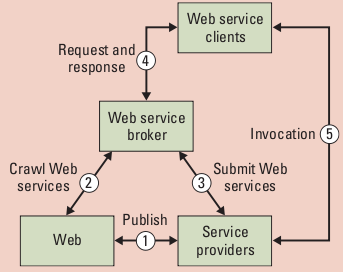
\includegraphics[scale=0.7]{images/web-service-broker.png}
	\captionof{figure}{Arquitetura do \textit{Web Service Broker} \cite{al2008toward}}
	\label{fig:web-service-broker}
\end{center}


Neste modelo, os provedores publicam informações sobre seus serviços em um diretório UDDI ou em motores de busca (passo 1). O WSB coleta informações sobre os \textit{Web Services} disseminados pela Web e continuamente monitora seus comportamentos, baseado em parâmetros de QWS (passo 2). O WSB não requer nenhuma intervenção humana, sendo totalmente automatizado. Provedores também podem submeter seus \textit{Web Services} ao WSB (passo 3). A interface do WSB permite que clientes localizem serviços, baseados em parâmetros de QWS (passo 4). Quando os clientes recebem mensagens de resposta, eles podem invocar os serviços (passo 5). É assumido que os serviços monitorados suportam invocação de operações sem cobrança de taxas ou assinaturas. A interface dos \textit{Web Services} deve suportar \textit{ping} para não sobrecarregar o sistema durante o monitoramente. O WSB realiza uma série de testes para determinar a disponibilidade de um determinado serviço, como verificar se o WSDL possui um endereço válido para um \textit{end point}.


\subsubsection{Conclusões}

O \textit{Web Service Broker} permitiu a coleta de informações sobre parâmetros de qualidade de serviço de diferentes \textit{Web Services}, que podem ser usados por instituições para busca de serviços relevantes, que atendam aos seus requisitos de qualidade de serviço.


%\subsection{\textit{Semantic Web Service Offer Discovery for E-Commerce} \cite{kopecky2008semantic}} \label{sec:sws-offer}

A Web Semântica é uma extensão da atual Web com descrições semânticas de dados e serviços que podem ser usados automaticamente por um computador em nome de seu usuário \cite{kopecky2008semantic}. Para tornar os \textit{Web Services} parte da Web Semântica, a área de pesquisa de Web Services Semânticos (\textit{Semantic Web Services}, SWS\nomenclature{SWS}{\textit{Semantic Web Services}}) tem como objetivo, aumentar o nível de automação ao redor dos \textit{Web Services}. Automação de SWS é suportada por descrições semânticas processáveis por computador, que captura aspectos importantes do significado de operações e mensagens de serviços. \cite{kopecky2008semantic}

A automação dos Web Services é realizada em um \textit{Semantic Execution Environment} (SEE\nomenclature{SEE}{\textit{Semantic Execution Environment}}). Este ambiente é responsável por receber um objetivo concreto de um usuário e cumprí-lo, localizando e usando apropriados WSs disponíveis, como apresentado na Figura \ref{fig:SEE}.

\begin{center}
	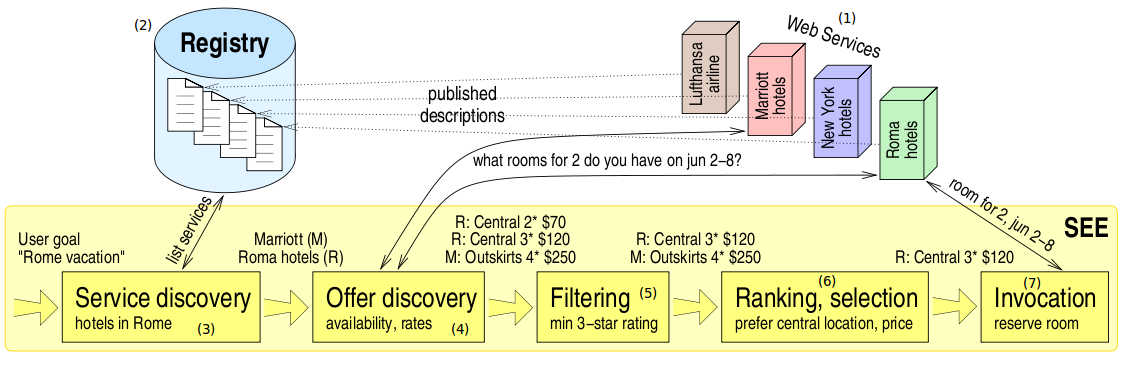
\includegraphics[width=1\textwidth]{images/see.png}
	\captionof{figure}{Automação de tarefas em um \textit{Semantic Execution Environment} (adaptada de \cite{kopecky2008semantic}).}
	\label{fig:SEE}
\end{center}

Na Figura \ref{fig:SEE}, existem alguns serviços registrados (1) em um repositório (2). O usuário deseja uma vaga em um hotel em Roma (3), então o SEE busca uma lista de serviços registrados de hotéis em Roma. Continuando, o SEE descobre ofertas\footnote{O termo "descoberta de ofertas" é cunhado pelos autores em \cite{kopecky2008semantic} como um sinônimo de "descoberta de serviços", apenas para fazer distinção entre o \textit{Web Service} em si e os serviços disponibilizados por ele (as operações).}, baseado em preços e disponibilidade de quartos, interagindo com os serviços encontrados (4). Em seguida o SEE, baseado nos critérios do usuário, filtra os resultados para que sejam obtidos apenas os hotéis que tenham classificação mínima de três estrelas (5) e classifica-os, selecionando aquele que tenha o menor preço e esteja no centro da cidade (6). Após a seleção, é feita a invocação do serviço para reserva de um quarto (7).

Existem alguns \textit{frameworks} de SWS que suportam automação, como esboçado na Figura \ref{fig:SEE}; os maiores são o \textit{Web Service Modeling Ontology} (WSMO)\footnote{\url{http://www.wsmo.org}}\nomenclature{WSMO}{\textit{Web Service Modeling Ontology}} e o \textit{Semantic Markup for Web Services} (OWL-S)\footnote{\url{http://www.w3.org/Submission/OWL-S}, no entanto, nenhum deles suporta a descoberta de oferta. Desta forma, o trabalho apresentado em  \cite{kopecky2008semantic} propõe o WSMO-Lite, um \textit{framework} leve para SWS, que adiciona anotações semânticas à descrição de Web Service.

\subsubsection{Descoberta de Oferta de Serviço}

O objetivo da descoberta de oferta de serviço é descobrir, classificar e selecionar serviços. A descoberta retorna um conjunto de serviços que podem potencialmente atingir o objetivo do usuário.  A descoberta de oferta é a interação com estes serviços (ou provedores de serviços), que resulta em um conjunto de ofertas, de onde deve-se selecionar alguma oferta relevante para o usuário. Este conjunto é então filtrado e classificado, de acordo com critérios do usuário, para permitir a seleção do melhor serviço. Por último, o serviço selecionado é consumido. \cite{kopecky2008semantic}

\subsubsection{Anotações Semânticas em WS com WSMO-\textit{Lite}}

Descoberta de oferta semântica pode, opcionalmente, ser capaz de realizar comunicação com qualquer WS que proveja operações para busca de informações sobre seus serviços. Para conseguir isto, o motor de descoberta de oferta precisa de uma descrição da interface do serviço, para ver quais operações o serviço contém, que podem ser usadas para obter informações de ofertas; e uma descrição dos dados trocados, para entender as ofertas e ser capaz de compará-las com o objetivo do usuário. \cite{kopecky2008semantic}

Qualquer serviço, descrito em WSDL, tem uma interface que consiste de operações. O WSMO-\textit{Lite} anota a interface e operações do \textit{Web Service} com semânticas funcionais, e os parâmetros de entrada e saída das operações são anotados com semânticas de informação.

O \textit{framework} utiliza a semântica de operações seguras do WSDL 2.0\footnote{Segundo a W3C\cite{w3c-wsdl-safety}, uma interação segura é aquela em que o cliente não tem nenhuma obrigação ao utilizar um determinado serviço, não estando obrigado a realizar nenhum contrato com o provedor. Por exemplo, ao acessar um método para consulta de preços de quartos em um hotel, o cliente não está obrigado a realizar a reserva. Métodos seguros são definidos no WSDL com o uso do atributo \textit{safe}.} para obter uma lista de métodos que fornecem informações sobre serviços disponibilizados (como métodos para obtenção de classificação de estrelas de um hotel, valores das reservas, disponibilidade, etc.

\subsubsection{Conclusões}

A proposta apresentada em \cite{kopecky2008semantic} implementa um \textit{framework} denominado WSMO-\textit{Lite}, para incluir anotações semânticas leves em arquivos WSDL, para permitir a automatização de descoberta de ofertas. O \textit{framework} é baseado em um \textit{Semantic Execution Environment} que permite que um usuário encontre ofertas de serviços, baseado em objetivos por ele definidos. A arquitetura apresentada é bastante interessante pois permite não somente a descoberta de serviços, mas a automatização da realização dos objetivos do usuário, como reservar um quarto de hotel, baseado em critérios como total de estrelas do hotel, preço e localização, sem que o usuário precise acessar cada um dos serviços disponibilizados para ele mesmo decidir qual o melhor.

%\subsection{Comparação entre as Propostas de Descoberta de Serviços}

Na Tabela \ref{tab:comparacao-descoberta-ws} é apresentada uma comparação entre as propostas de descoberta de serviços abordadas na Seção \ref{sec:propostas-descoberta-ws}. A primeira coluna apresenta as propostas avaliadas. A segunda indica se a arquitetura utilizada para a descoberta de serviços é distribuída ou não. A terceira indica se os repositórios de registro de serviço detectam e classificam os serviços inativos, para que somente os serviços ativos sejam disponibilizados aos usuários. A quarta indica como é feito o processo de registro/descoberta de serviços. A quinta informa se a proposta detecta, automaticamente, modificações nos serviços registrados. A sexta coluna indica se a proposta utiliza descrições semânticas para estender
o documento WSDL. A sétima indica se a proposta utiliza parâmetros de QoS para seleção de serviços.

\begin{center}
{\tiny
  \begin{tabular}{|p{2.5cm}|p{0.6cm}|p{2.5cm}|p{2.9cm}|p{3.5cm}|p{1.5cm}|p{0.4cm}|} %{|l|c|l|l|l|c|c|}
  \hline
	\textbf{Proposta} &\textbf{Distrib} &\textbf{Classifica Serviços Inativos}\par \textbf{Automaticamente} & 
	\textbf{Registro dos Serviços} &\textbf{Rastreia alterações nos WSs}\par \textbf{Automaticamente} &
	\textbf{Semântica} & \textbf{QoS}   \\

   \hline
	\textit{A Novel Interoperable Model}\par \textit{of Distributed UDDI} \cite{wu2008novel}\par Seção \ref{sec:novel-model-uddi} 
	& Sim 
	& Sim & Manual,\par realizado pelo provedor. 
	& Não.\par Somente os provedores podem informar sobre alterações. 
	& Não & Não\\

    \hline
	\textit{Active Web Service} \cite{treiber2007active}\par Seção \ref{sec:active-ws-reg} 
	& Sim 
	& Não.\par Somente os provedores podem informar sobre a desativação de um serviço, atualizando o \textit{feed} RSS/Atom.  
	& Manual.\par Os clientes devem assinar o \textit{feed} RSS/Atom do provedor, 
	para serem informados de novos serviços e atualizações,
	ou utilizar sites agregadores de \textit{feeds} de diversos provedores. 
	& Não.\par As alterações só são detectadas a partir do momento que o provedor 
	atualiza o \textit{feed} RSS/Atom de publicação dos serviços. 
	& Não & Não\\

    \hline
	 \textit{A New Description Model}\par \textit{of Web Service} \cite{wu2009new}\par Seção \ref{sec:ws-description-model}  
	& NI 
	& Não Informado 
	& Automático,\par mas não é informado como, apenas cita que com uso de OWL-S isto é possível 
	& Automático,\par mas não é informado como, apenas cita que com uso de OWL-S isto é possível 
	& Sim,\par usando OWL-S. & Sim\\

    \hline
	\textit{Finding Web Services} \cite{lausen2007finding}\par Seção \ref{sec:finding-ws} 
	& NI
	& Sim & Automatizado, por meio de um \textit{crawler} específico 
	& Não informado,\par mas o \textit{crawler} pode detectar tais alterações e atualizar as descrições do serviço.
	& Sim,\par obtendo informações implícitas (como a localização, obtida a partir do IP) e explícitas (informadas no WSDL) 
	& Sim \\

    \hline
	\textit{Toward Quality-Driven}\par \textit{Web Service Discovery} \cite{al2008toward}\par Seção \ref{sec:quality-driven-discovery} 
	& NI & Sim
	& Automatizado, por meio de Web \textit{crawling} usando um componente denominado \textit{Web Service Broker}, ou registro manual.
	& Não informado,\par mas o \textit{Web Service Broker} pode detectar tais alterações e atualizar as descrições do serviço.
	& Não & Sim \\

    \hline
   	 \textit{Semantic WS Offer Discovery}\par \textit{for E-Commerce} \cite{kopecky2008semantic}\par Seção \ref{sec:sws-offer} 
	 & NI & Não Informado & Manual.\par A descoberta é feita a partir dos serviços registrados, baseado em critérios do usuário.
	 & Não Informado & Sim,\par usando WSMO-\textit{Lite}, baseado no WSMO. & NI \\

    \hline
	\end{tabular}
	*NI = Não Informado

    \captionof{table}{Comparação das Propostas de Descoberta de Serviços}
    \label{tab:comparacao-descoberta-ws}
}
\end{center}


%WS em TVD
%input no lugar de include evita a quebra de linha inserida por este
%\section{\textit{Web Services} em Ambientes de TV Digital Interativa}

Como visto no Capítulo \ref{cap:ws}, a tecnologia de \textit{Web Services} permite a integração entre sistemas heterogêneos, de uma forma simples e padronizada, utilizando protocolos e padrões já estabelecidos na Web. Com a TV Digital Interativa (TVDI) não é diferente, o uso dos \textit{Web Services} traz muitas facilidades e benefícios. Pelo fato de aplicações de TV Digital (TVD) serem principalmente implementadas em um modelo \textit{desktop}, e pela baixa capacidade de recursos dos receptor de TVD, os \textit{Set-top boxes}, a construção de aplicações distribuídas com uso de \textit{Web Services} libera o receptor de realizar processamentos pesados, que podem ser delegados a um WS. Desta forma, o uso dos WSs permite ainda, que as aplicações de TVD que fazem uso desta tecnologia, tenham um tamanho reduzido, devido às regras de negócio serem implementadas no WS, necessitando de menos largura e banda para transmitir as mesmas, e menor espaço em memória para armazená-las.

Tendo em vista os benefícios dos WSs para aplicações de TV Digital, algumas propostas surgem para provimento e descoberta de serviços em tal ambiente, como apresentado nas seções seguintes.

\subsection{Provendo WSs em Ambientes de TVD Móvel \cite{vilas2007providing}} %Providing WSs over DVB-H Mobile Virtual Web Services

Com o crescimento do acesso à Internet a partir de dispositivos móveis, tendência mundial também observada no Brasil 
\cite{banda-larga-movel-olhar-digital}, é cada vez mais comum o acesso a serviços a partir de tais dispositivos. No entanto, devido à reduzida capacidade da maioria destes dispositivos, as aplicações móveis acessadas a partir deles, devem ser tão simples quanto possível. Desta forma, o trabalho em \cite{vilas2007providing} apresenta um \textit{framework} para reduzir a complexidade de tais aplicações, criando \textit{Web Services} Virtuais. Estes são grupos de um ou mais serviços, permitindo que o dispositivo móvel possa utilizá-los, com transparência de localização dos serviços, além de permitir balanceamento de carga e resiliência.

Outro objetivo do trabalho apresentado em \cite{vilas2007providing}, é permitir a desvinculação das aplicações móveis de um provedor de serviços específico. Como, convencionalmente, aplicações clientes são atreladas a um determinado provedor, a complexidade de troca de provedor em tempo de execução pode ser excessiva para um dispositivo móvel. Além do mais, em dispositivos móveis, normalmente a troca do provedor de serviços requer a troca e reconfiguração da aplicação cliente, o que pode ser incômodo para o usuário.

Com isto, em \cite{vilas2007providing} é apresentada a proposta de \textit{Virtual Web Services} (VWSs)\nomenclature{VWS}{\textit{Virtual Web Service}}. Um VWS é um \textit{Web Service} padrão, que agrupa um ou mais serviços, criando uma camada de abstração entre os clientes móveis e os provedores de serviços, escondendo dos clientes a complexidade, disponibilidade e localização dos serviços. A Figura \ref{fig:virtual-ws} apresenta um cenário de uso de VWS.

\begin{center}
	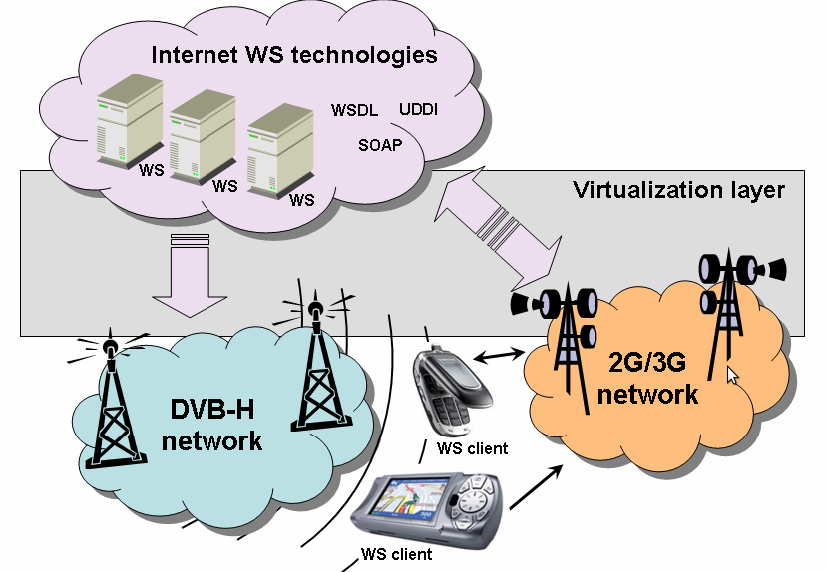
\includegraphics[width=0.8\textwidth]{images/virtual-ws-scenario.png}
	\captionof{figure}{Cenário de uso de um \textit{Virtual Web Service} \cite{vilas2007providing}}
	\label{fig:virtual-ws}
\end{center}

Diferentes provedores que fornecem um mesmo serviço, apesar de todos usarem XML para representar os dados trocados, podem receber diferentes tipos de parâmetros e devolver respostas em diferentes formatos. Em \cite{vilas2007providing} é apresentado um exemplo de serviço para obtenção das condições do tráfego em determinado local. Assim, um serviço pode fornecer as condições de fluxo do trânsito numa escola de 1 a 5, outro pode fornecer valores textuais como "Devagar", "Congestionado" e "Fluxo Livre". Desta forma, com o uso de VWS, as aplicações clientes não precisam se preocupar com estes detalhes de implementação de cada serviço. O VWS cria uma interface única para acesso aos diferentes serviços de informações de trânsito, sendo ele mesmo um \textit{Web Service} no padrão SOAP, que possui uma interface descrita por meio de um WSDL padrão.

Um VWS permite ainda a seleção de serviços baseada em fatores de QoS, permitindo ainda, a implementação de mecanismos de \textit{cache}. Tal mecanismo permite que resultados de invocações a um serviço sejam armazenadas no servidor do VWS, para que invocações futuras, usando os mesmos parâmetros de entrada, recebam o resultado já processado e armazenado previamente, podendo reduzindo o tempo de resposta das requisições em \textit{cache}.

\subsubsection{Conclusões}

A solução apresentada em \cite{vilas2007providing} é bastante relevante, por agrupar serviços similares, disponibilizados por diferentes provedores, em uma camada de abstração denominada \textit{Virtual Web Service}. Esta camada permite a seleção de serviços baseada em fatores de QoS, além de prover transparência de localização e resiliência. Outro ponto forte é o uso dos protocolos padrões de \textit{Web Services}, como HTTP, WSDL e SOAP. Desta forma, para as aplicações clientes, não há diferença entre um \textit{Virtual Web Service} e um \textit{Web Service} convencional.

%\subsection{Descoberta de Serviços em Ambientes de TVDI \cite{borges2007arquitetura}} 

Um ambiente de TV Digital Interativa (TVDI)\nomenclature{TVDI}{TV Digital Interativa} pode oferecer, aos seus usuários, uma grande quantidade de serviços. Tais serviços podem ser acessados pelo Guia Eletrônico de Programação (\textit{Eletronic Program Guide}, EPG \nomenclature{EPG}{\textit{Eletronic Program Guide}}). No entanto, muitos outros serviços podem ser disponibilizados por meio do acesso ao canal de retorno, que não são catalogados pelo EPG. Tecnologias como Jini, \textit{Service Location Protocol} e \textit{Universal Plug and Play} podem ser utilizadas para descoberta de serviços em infra-estruturas híbridas como a de TVDI. Elas permitem que os usuários tomem conhecimento dos serviços que lhe são disponibilizados.

Tendo em vista as diferentes tecnologias existentes, em \cite{borges2007arquitetura} é apresentada uma proposta para possibilitar o uso transparente, independente de localização, de serviços providos por diferentes protocolos de descoberta. É apresentada uma arquitetura, a ser incorporada no middleware dos receptores de TVD\nomenclature{TVD}{TV Digital}.

\subsubsection{Protocolos de Descoberta de Serviços} \label{service-discovery-protocols}

Protocolos para descoberta dinâmica de serviços tem sido criados para liberar o usuário da necessidade de conhecer o endereço do serviço e efetuar configurações para utilizá-lo. Sistemas para descoberta permitem que sejam divulgados serviços, sendo que os clientes podem buscar tais serviços com base em seus atributos publicados.

Arquiteturas existentes para descoberta de serviços são compostas, de pelo menos, dois elementos: os provedores de serviços e os usuários de serviços. Em algumas arquiteturas existe um elemento intermediário, responsável por gerenciar os serviços, como em \cite{al2008toward}. Em sistemas sem um gerenciador, as requisições dos usuários são enviadas diretamente aos provedores. Em sistemas com gerenciador, inicialmente os provedores registram seus serviços no gerenciador, e/ou este varre a Web em busca de serviços públicos, como em \cite{al2008toward}.

%\subsubsubsection{Jini}
\textbf{Jini}

O projeto Jini, inicialmente desenvolvido pela \textit{Sun Microsystems}, atualmente suportado pela \textit{Apache Software Foundation} e denominado \textit{Apache River}, é uma arquitetura orientada a serviços, que define um modelo de programação, que explora e estende a tecnologia Java, para habilitar a construção de sistemas distribuídos seguros, consistindo de federações de serviços e clientes. A tecnologia Jini também pode ser usada para construir sistemas de rede adaptativos, escaláveis, evolutívos e flexíveis, como tipicamente requerido em ambientes de computação dinâmica \cite{apache-river}.

A arquitetura Jini é desenvolvida em linguagem Java e utiliza o modelo de objetos distribuídos \textit{Remote Method Invocation} (RMI)\nomenclature{RMI}{\textit{Remote Method Invocation}} e possibilita que as referências dos objetos remotos sejam carregadas entre receptores com a \textit{Java Virtual Machine} (JVM)\nomenclature{JVM}{\textit{Java Virtual Machine}}. Ela possui ainda um sistema de alerta sobre a disponibilidade de serviços buscados pelo usuário.

A Figura \ref{fig:jini-sequence-diagram} apresenta um diagrama de sequências, mostrando algumas mensagens trocadas na interação entre os componentes da arquitetura Jini.

\begin{center}
	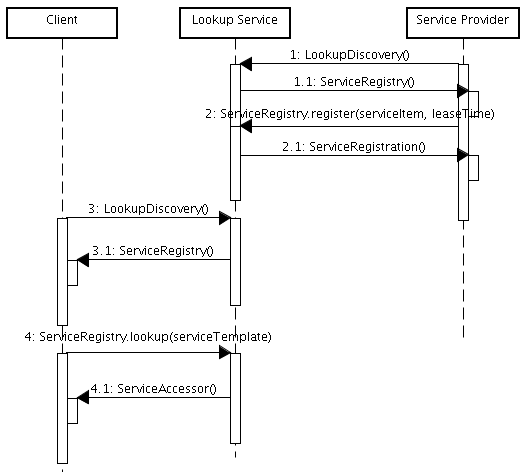
\includegraphics[scale=0.6]{images/jini-sequence-diagram.png}
	\captionof{figure}{Diagrama de sequência para componentes Jini (adaptada de \cite{borges2007arquitetura}).}
	\label{fig:jini-sequence-diagram}
\end{center}

Tanto os clientes quanto os provedores de serviços precisam descobrir o endereço do \textit{Lookup Service}, enviando uma mensagem \textit{multicast} (\textit{LookupDiscovery}) para localizar este servidor. O \textit{Lookup Service} é responsável por gerenciar os serviços de diferentes provedores, interligando os clientes a estes.
Os provedores de serviço devem registrar seus serviços junto ao \textit{Lookup Service} (\textit{ServiceRegistry.register}), para que os clientes possam utilizar tais serviços. E por fim, os clientes podem buscar por um determinado serviço (\textit{ServiceRegistry.lookup}), baseado em critérios definidos por ele.

%\subsubsubsection{\textit{Service Location Protocol} (SLP)}
\textbf{\textit{Service Location Protocol} (SLP)}

O protocolo SLP\nomenclature{SLP}{\textit{Service Location Protocol}} foi desenvolvido pelo \textit{Internet Engineering Task Force} (IETF) \nomenclature{IETF}{\textit{Internet Engineering Task Force}} para permitir a descoberta de serviços, sem que os clientes necessitem conhecer sua localização \cite{borges2007arquitetura}. Também baseado em uma arquitetura de 3 camadas, como o Jini, sendo seus elementos:

\begin{itemize}
	\item \textit{User Agents} (UA): cliente que realiza a busca por serviços;
  \item \textit{Service Agents} (SA): anuncia e controla os serviços por ele disponibilizados (equivalente ao \textit{Service Provider} na arquitetura Jini);
  \item \textit{Directory Agents}: mantém uma lista dos serviços nele registrados, intermediando as interações entre os UAs e os SAs (equivalente ao \textit{Lookup Service} na arquitetura Jini).
\end{itemize}

A troca de mensagens usando o protocolo SLP também é semelhante ao que ocorre na arquitetura Jini, como pode ser visto na Figura \ref{fig:slp-flow-message}.

\begin{center}
	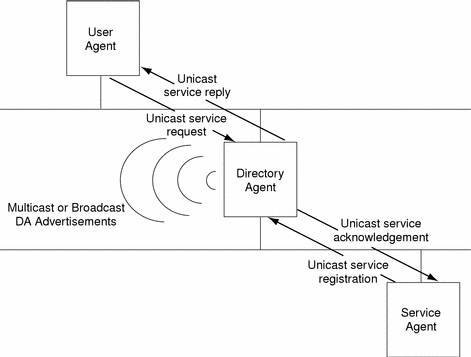
\includegraphics[width=0.7\textwidth]{images/slp-flow-message.png}
	\captionof{figure}{Troca de mensagens entre componentes do protocolo SLP \cite{slp-admin-guide}}
	\label{fig:slp-flow-message}
\end{center}

%\subsubsubsection{Universal Plug and Play (UPnP)}
\textbf{Universal Plug and Play (UPnP)}

O UPnP\nomenclature{UPnP}{\textit{Universal Plug and Play}} é um conjunto de protocolos para descoberta de serviços, desenvolvido por um consórcio de empresas, liberado pela \textit{Microsoft}. Ele define uma arquitetura para estender o modelo de periféricos \textit{Microsoft Plug and Play}, visando um modelo altamente dinâmico para a integração com vários dispositivos de redes de diferentes fabricantes \cite{borges2007arquitetura}. A arquitetura UPnP define protocolos de comunicação entre controladores e dispositivos, para descoberta, descrição, controle, eventos e apresentação, sendo eles: \textit{Simple Service Discovery Protocol} (SSDP), \textit{General Event Notification Architecture} (GENA), SOAP, HTTP, XML, TCP/IP e UDP \cite{borges2007arquitetura}. Um grande ponto forte do protocolo é a utilização de padrões como HTTP, XML e SOAP, permitindo que a troca de mensagens seja feita utilizando protocolos Web padronizados, o que evita problemas com portas bloqueadas em \textit{Firewalls}.

%\subsubsubsection{\textit{Service Discovery Protocol} (SDP)}
\textbf{\textit{Service Discovery Protocol} (SDP)}

O SDP\nomenclature{SDP}{\textit{Service Discovery Protocol}} faz parte das especificações \textit{Bluetooth} (IEEE 802.15.1), e é utilizado para descoberta de serviços em uma \textit{Personal Area Network} (PAN)\nomenclature{PAN}{\textit{Personal Area Network}}, sendo uma arquitetura de duas camadas, contendo dois agentes: o \textit{SDP Server} e o \textit{SDP Client}. 

\subsubsection{Solução Proposta}

Em \cite{borges2007arquitetura} é apresentada uma arquitetura para descoberta de serviços em ambientes de TVDI. O trabalho cita um caso de uso de uma pizzaria que deseja fazer uma promoção pela TVD, por um determinado período de tempo. A aplicação deve ser disponibilizada via \textit{broadcast} para seus usuários e a promoção deve durar um tempo determinado. Como o total de usuários que venham a utilizar a aplicação pode ser alto, isto pode sobrecarregar o serviço. Desta forma, é necessário um mecanismo de balanceamento de carga para distribuir os pedidos de pizza entre as diversas filiais da rede de pizzarias que promoveu a promoção, onde cada filial estaria provendo o serviço de pedidos de pizza pela TVDI. Além disto, \cite{borges2007arquitetura} cita que a aplicação pode estar disponível para usuários com dispositivos móveis. Desta forma, é necessário que a descoberta de serviços, disponíveis na localidade atual do usuário, seja feita sem a necessidade de configurações manuais.

O trabalho em \cite{borges2007arquitetura} apresenta uma proposta de arquitetura para descoberta de serviços em TVDI, que contempla os requisitos citados anteriormente.

%\subsubsubsection{Arquitetura da Solução}
\textbf{Arquitetura da Solução}

A arquitetura proposta em \cite{borges2007arquitetura} é composta por três camadas, descritas a seguir.

\begin{itemize}
	\item Aplicações: camada contendo as aplicações clientes executados no receptor digital (fixo, móvel ou portátil).
  \item \textit{Middleware}: encapsula os componentes para busca, atualização e registro de serviços, além das funcionalidades de tempo de disponibilização dos serviços e balanceamento de carga.
  \item Protocolos de Descoberta de Serviços: infra-estrutura para acesso aos diversos protocolos de descoberta de serviços, tratados na Seção \ref{service-discovery-protocols}.
\end{itemize}

A Figura \ref{fig:arq-descoberta-servicos-tvdi} apresenta a arquitetura da solução apresentada em \cite{borges2007arquitetura}.

O tipo de protocolo de descoberta de serviços é irrelevante para a aplicação. Para tornar este acesso transparente, foram desenvolvidos componentes no \textit{middleware}, que são acessados pela aplicação, a partir de uma API desenvolvida. O acesso aos diferentes protocolos de descoberta pode ser feito por meio de um canal de retorno.

Os componentes implementados, que devem estar presentes na camada de \textit{middleware}, sendo incorporados a ele, são definidos a seguir.

\begin{itemize}
	\item Busca: possibilita a busca de serviços disponibilizados para o ambiente de TVDI, independente do protocolo de descoberta subjacente.
  \item Registro: possibilita que um usuário disponibilize serviços armazenados em seu receptor digital, a outros usuários.
  \item Atualização: possibilita que altere ou torne indisponível um serviço.
  \item Temporalidade: permite definir um período de tempo no qual o serviço estará disponível.
  \item Balanceamento: permite balancear a carga de acessos a um determinado serviço, para diferentes provedores do mesmo serviço.
\end{itemize}

\begin{center}
	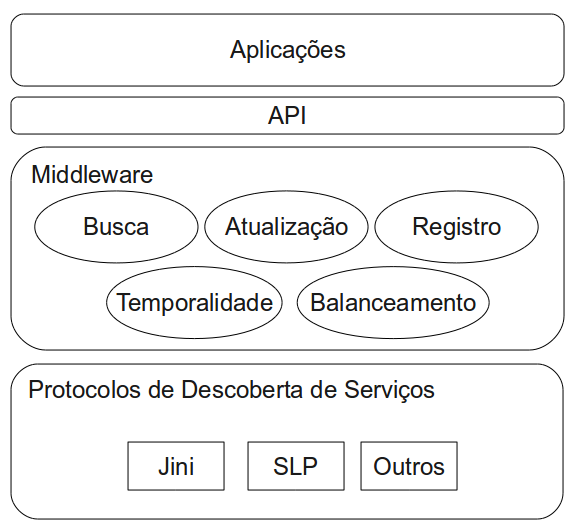
\includegraphics[width=0.70\textwidth]{images/arquitetura-descoberta-servicos-tvdi.png}
	\captionof{figure}{Arquitetura para Descoberta de Serviços em TVDI \cite{borges2007arquitetura}}
	\label{fig:arq-descoberta-servicos-tvdi}
\end{center}

\subsubsection{Conclusões}

A arquitetura apresentada em \cite{borges2007arquitetura} permite a descoberta de serviços em ambientes de TVDI, tornando transparente para as aplicações, o tipo de protocolo de descoberta utilizado. A arquitetura é baseada em três camadas, como convencionalmente encontrado em outras propostas citadas, e possui recursos importantes como balanceamento de carga e opção para definir o tempo de disponibilidade dos serviços. Um recurso bastante interessante é a possibilidade de tornar conversores digitais de usuários em provedores de serviços, utilizando uma infra-estrutura já existente para fornecer serviços, podendo estes serem replicados em diferentes conversores, permitindo o balanceamento de carga entre eles.


%E-Commerce/Security
%input no lugar de include evita a quebra de linha inserida por este
%\section{Comércio Eletrônico}


\subsection{\textit{E-Commerce Security}} \label{e-commerce-secutiry}

Comércio eletrônico (\textit{E-Commerce}\nomenclature{E-Commerce}{Comércio Eletrônico}) é a compra e venda de mercadorias pela Internet. Atividades comerciais na Internet tem crescido exponecialmente nos últimos anos \cite{al2008commerce}. No atual mercado globalizado, qualquer negócio, para ser competitivo, necessita de políticas de segurança abrangentes, em conformidade com seus parceiros, para prover ambientes seguros para a realização de atividades de comércio eletrônico \cite{al2008commerce}.

Para prover tais ambientes seguros, uma Infra Estrutura de Chaves Públicas - ICP\nomenclature{ICP}{Infra Estrutura de Chaves Públicas} (\textit{Public Key Infrastructure}, PKI\nomenclature{PKI}{\textit{Public Key Infrastructure}}) pode ser utilizada para estabelecer comunicações seguras em uma rede, utilizando criptografia de chaves públicas. ICP define um ambiente onde usuários podem trasmitir certificados que os identificam \cite{al2008commerce}. 

Aplicações de \textit{E-Commerce} também podem funcionar \textit{Secure Electronic Transfer} (SET)\nomenclature{SET}{\textit{Secure Electronic Transfer}} ou \textit{Secure Socket Layer} (SSL)\nomenclature{SSL}{\textit{Secure Socket Layer}} para criptografia de tranmissões de dados utilizando os protocolos TCP/IP \cite{al2008commerce}.

No ciberespaço, tanto clientes quanto vendedores tem dificuldades em prover sua identifidade um para o outro com certeza, particularmente durante a primeira transação. Algumas questões levantadas em \cite{al2008commerce}, apresentadas a seguir, descrevem problemas que afetam transações comerciais em uma rede de computadores pública, como a Internet: Como o comprador transmite informações sensíveis para o vendedor? Como o vendedor conhece uma ordem de compra legítima? Como ambas as partes sabem que um terceiro mal intecionado não copiou ou alterou as informações da transação? 

\cite{al2008commerce} indica que clientes precisam garantir que:
\begin{itemize}
	\item eles estão se comunicando com o servidor correto;
  \item o que eles enviam é entregue sem modificações;
  \item eles podem provar que enviaram a mensagem;
  \item somente o destinatário desejado pode ler a mensagem; e
  \item a entrega é garantida.
\end{itemize}

No lado dos vendedores, eles precisam ter garantia que \cite{al2008commerce}:

\begin{itemize}
	\item eles estão se comunicando com o cliente correto;
	\item o conteúdo da mensagem recebida está correto;
	\item a identidade do autor não pode ser falsificada;
	\item somente o autor declarado pode realmente ter escrito a mensagem; e
	\item eles confirmam o recebimento da mensagem.
\end{itemize}

Em \cite{jiang2007line} são citados alguns fatores de segurança que aplicações de \textit{E-Commerce} devem considerar, como: confidencialidade, integridade, validade e não repúdio da informação e autenticidade.

Ambas as partes também não podem repudiar uma mensagem que enviaram \cite{jiang2007line}, por exemplo, um cliente legítimo que realizou um pedido de compra não tem como negar que o fez. O receptor deve ter como confirmar que a mensagem recebida é realmente do emissor informado na mensagem, e o emissor deve ter garantia de que somente o destinatário designado poderá ler a mesma \cite{jiang2007line}. São necessários mecanismos para identificar a integridade das informações trocadas, para saber quando as mesmas foram alteradas \cite{jiang2007line}, intecionalmente, devido a ação de \textit{crackers} ou não, devido a falhas de hardware e software.

Todos as preocupações listadas acima podem ser resolvidas usando alguma combinação de métodos criptográficos e métodos de certificado. Os tipos de risco resultante de inadequada segurança, segundo \cite{al2008commerce}, são:

\begin{itemize}
	\item bugs ou problemas de configurações incorretas no servidor Web, que podem causar roubo de documentos confidenciais;
	\item brechas de segurança no lado do cliente, que podem comprometer sua privacidade e danificar seu sistema;
	\item interceptação de dados enviados do cliente para o servidor, e vice-versa. Isto é possível em qualquer parte do caminho entre a rede do cliente e a o servidor, na rede do provedor de Internet do usuário ou outros provedores regionais.
\end{itemize}

\subsubsection{Políticas de Medidas de Segurança em \textit{E-Commerce}}

Segundo \cite{al2008commerce}, existem três diferentes políticas usadas para garantir e medir a segurança em ambientes de \textit{E-Commerce}, que são: privacidade, criptografia e certificados.

%\subsubsection{Política de Privacidade}
\textbf{Política de Privacidade}

Política de Privacidade são utilizadas para arquitetar a forma em que uma companhia coleta, usa, protege dados es escolhas que eles oferecem aos consumidores quando suas informações pessoais são utilizadas. Baseados nessa política, consumidores podem determinar se e com qual extensão eles desejam disponibilizar informações para a companhia.

%\subsubsection{Criptografia}
\textbf{Criptografia}

Sistemas de cifragem (criptografia) são classificados em duas classes, apresentadas a seguir.


\textbf{Sistemas de Chave Secreta}

A criptografia de chave secreta é o mais antigo método criptográfico, tendo dois principais tipos: a cifragem por transporte e por substituição. O primeiro criptografa a mensagem original alterando a ordem dos caracteres. O segundo substitui os caracteres da mensagem por outros. Em ambos os casos, o emissor e o receptor compartilham a mesma chave secreta. O algoritmo de chave secreta mais amplamente utilizado atualmente é o \textit{Data Encryptation Standard} (DES)\nomenclature{DES}{\textit{Data Encryptation Standard}}, que funciona com uma chave secreta de 56 bits e 16 iterações para transformar um bloco de texto plano em texto cifrado.

\textbf{Sistemas de Chave Pública}

A criptografai de chave pública foi desenvolvida para resolver o problema de distribuição de chaves secretas. O primeiro algoritmo foi publicamente descrito em 1976 pelo professor Martin Hellman, da Universidade de Stanford, e seu aluno graduando Whitfield Diffie. Tais métodos utilizam duas diferentes chaves matematicamente relacionadas. Uma chave é usada para criptografar os dados, e a segunda para descriptografar. O segundo problema que Diffie ponderou foi o de "assinaturas digitais". O esquema de Rivest Shamir-Adleman (RSA) é o mais conhecidamente aceito e implementado algoritmo de propósito geral para criptografia de chave pública. O esquema é uma cifra de bloco em que o texto plano e o texto cifrado são inteiros entre 0 e n-1 for algum n. Um tamanho típico para n é 1024 bits, ou 309 dígitos decimais. O tamanho de bloco deve ser menor ou igual a log2(n). Segundo \cite{al2008commerce}, a criptografia e a descriptografia são da seguinte forma, para algum texto plano M e um texto cifrado C:
\begin{center}
	\begin{equation}
		C=M^e\:mod\:n%\: incluir espaço entre elementos da equação
	\end{equation}
	\captionof{equation}{Cifragem com RSA \cite{al2008commerce}}
	\label{eq:rsa-cifragem}
\end{center}

\begin{center}
	\begin{equation}
    %\: incluir espaço entre elementos da equação
		M \: = \: C^d \: mod \: n \: = \: (M^e)^d \: mod \: n \: = \: M^{ed} \: mod \: n 
	\end{equation}
	\captionof{equation}{Decifragem com RSA \cite{al2008commerce}} 
	\label{eq:rsa-decifragem}
\end{center}

Ambos emissor e receptor devem conhecer o valor de \textit{n}. O emissor conhece o valor de \textit{e}, e somente o receptor conhece o valor de \textit{d}. Assim, segundo \cite{al2008commerce}, este é um algoritmo de chave pública com:
\begin{itemize}
	\item uma chave pública de $ KU=\{e,n\} $
	\item uma chave privada de $ KR=\{d,n\} $
\end{itemize}

%\subsubsection{Certificado}
\textbf{Certificado}

Certificados associam identidade, autoridade, chave pública e outras informações do usuário. Para a maioria das aplicações de \textit{E-Commerce}, certificados usam um formato definido pelo \textit{International Telecommunication Union - Telecomunication Standardization Sector} (ITU-T)\nomenclature{ITU-T}{\textit{International Telecommunication Union - Telecomunication Standardization Sector}}, tal como a recomendação X.509. Segundo \cite{al2008commerce}, certificados X.509 contêm informações como:
\begin{itemize}
	\item nome, identificação e chave pública do proprietário do certificado;
	\item nome e identificação do emissor do certificado; 
	\item definições de limitações de uso, informações de políticas e período de validade do certificado.
\end{itemize}

Com uso de certificados digitais, compradores podem obter um certificado digital pessoal para provar sua identidade para um Web \textit{site}, mas os vendedores é que realmente precisam de certificados para provar sua identidade para os compradores.

\subsubsection{\textit{Pretty Good Privacy} (PGP)}\nomenclature{PGP}{\textit{Pretty Good Privacy}}

PGP provê um serviço de autenticação e confidencialidade que pode ser usado para \textit{e-mail} e aplicações de armazenamento de arquivos. Ele tem crescido explisivamente e é amplamente utilizado na atualidade. Segundo \cite{al2008commerce}, três razões podem ser citadas para isto:

\begin{itemize}
	\item ele é baseado em algoritmos que tem sobrevivido a extensas revisões públicas e são considerados extremamente seguros;
	\item ele tem uma ampla faixa de aplicabilidade;
	\item ele não foi desenvolvido nem é controlado por qualquer órganização governamental ou de padronização.
\end{itemize}

A atual operação do PHP consiste de cinco serviços: autenticação, confidencialidade, compressão, compatibilidade de e-mail e segmentação. A seguir são examinados os dois primeiros serviços, que podem ser utilizados para \textit{E-Commerce}.

%\subsubsection{Autenticação}
\textbf{Autenticação}

Transações na Internet são realizadas entre computadores geograficamente distantes. Desta forma as partes precisam reconhecer e confiar uma na outra \cite{jiang2007line}, especialmente em trasações de \textit{E-Commerce}, por envolverem dinheiro. Para isso, são necessários mecanismos de autenticação das partes.

Autenticação requer uma assinatura digital. O processo inicia com um resumo matemático denominado \textit{hash}, que age como uma impressão digital da mensagem. Assim, se a mensagem for alterada, se tornará incompatível com o \textit{hash} original. Este código \textit{hash} é criptografado com a chave primava do remetente e anexado à mensagem. Quando a mensagem é recebida, o código \textit{hash}, anexado a ela, é comparado com outro código \textit{hash} calculado pelo receptor. Chaves para assinaturas digitais são armazenadas em um diretório de chaves públicas, composto de "certificados" para todos os usuários. \cite{al2008commerce} Uma Autoridade Certificadora confiável gerencia e distribui estes certificados, para permitir a distribuição de chaves eletrônicas. O esquema de assinatura digital é apresentado na sequência abaixo e na Figura \ref{fig:pgp-authentication}.

\begin{itemize}
\item Geração de mensagem e assinatura pelo emissor:
	\begin{itemize}
		\item o emissor cria uma mensagem;
		\item algoritmo de \textit{hash} SHA-1 é usado para gerar um código \textit{hash} de 160 bits da mensagem;
		\item o código \textit{hash} é criptografado com RSA, usando a chave privada do emissor, e o resultado é acrescentado à mensagem.
    {\color{red}Este \textit{hash} criptografado é a assinatura digital da mensagem.} 
	\end{itemize}

\item Verificação da autenticidade da mensagem pelo receptor:
	\begin{itemize}
		\item o receptor usa RSA com a chave pública do emissor para descriptografar e recuperar o \textit{hash};
		\item o receptor gera um novo \textit{hash} a partir da mensagem, usando a chave pública do emissor e {\color{red}RSA},
    e compara este \textit{hash} com o \textit{hash} recebido e descriptografado. 
    Se os dois correspondem, a mensagem é aceita como autêntica.
	\end{itemize}
\end{itemize}

\begin{center}
	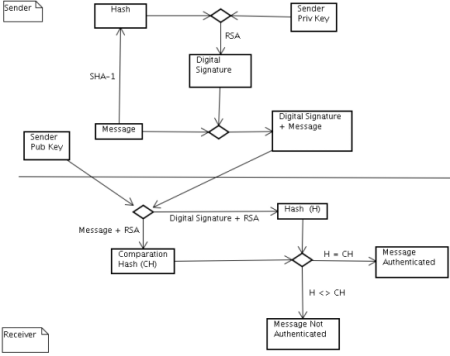
\includegraphics[scale=0.8]{images/pgp-authentication.png}
	\captionof{figure}{Autenticação em PGP}
	\label{fig:pgp-authentication}
\end{center}

A combinação de SHA-1 e RSA provê um efetivo esquema de assinatura digital. Devido à força do RSA, o receptor tem garantia de que somente o possuidor da chave privada pôde ter gerado a assinatura; e devido à força do SHA-1, ele tem garantia de que ninguém pode gerar uma mensagem que corresponda com o código \textit{hash} e com a assinatura da mensagem original. Embora assinaturas normalmente são anexadas à mensagem ou arquivo que elas assinam, assinaturas não anexadas também são suportadas. Estas podem ser armazenadas e transmitidas separadamente da mensagem que elas assinam.

%\subsubsection{Confidencialidade}
\textbf{Confidencialidade}

O emissor e receptor de uma mensagem precisam garantir a confidencialidade na troca de informações, principalmente em um ambiente de \textit{E-Commerce}. Assim, para previnir transações neste ambiente de roubo de informações, é preciso garantir que apenas usuários legítimos serão capazes de ver os dados\cite{jiang2007line}.

Confidencialidade é provida pela criptografia da mensagem a ser transmitida ou a ser armazenada localmente. O esquema é apresentado na sequência abaixo e na Figura \ref{fig:pgp-confidentiality}.

\begin{itemize}
  \item Geração de mensagem criptografada a ser aberta somente por um determinado destinatário
	\begin{itemize}
		\item o emissor gera uma mensagem e um número aleatório de 128 bits para ser usada como uma chave de sessão somente para esta mensagem;
		\item a mensagem é criptografada com esta chave de sessão;
		\item a chave de sessão é criptografada com RSA, usando a chave pública do receptor, e é acrescentada à mensagem criptografada.
    {\color{red}A chave de sessão criptografada é a assinatura digital da mensagem.} 
	\end{itemize}

  \item Descriptografia da mensagem recebida pelo destinatário objetivado pelo emissor
	\begin{itemize}
		\item o receptor usa RSA com sua chave privada para descriptografar e recuperar a chave de sessão;
		\item a chave de sessão é usada para descriptografar a mensagem, {\color{red}usando RSA}.
	\end{itemize}
\end{itemize}

\begin{center}
	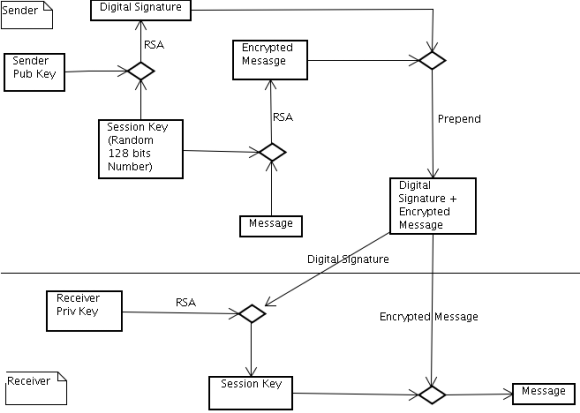
\includegraphics[scale=0.7]{images/pgp-confidentiality.png}
	\captionof{figure}{Confidencialidade em PGP}
	\label{fig:pgp-confidentiality}
\end{center}



%\subsection{\textit{Privacy in E-Commerce} \cite{berendt2005privacy}}

Privacidade é um dos requisitos básicos para sistemas de comércio eletrônico (\textit{E-Commerce}). Muitos dos recursos disponíveis para garantir tal privacidade foram relatados na Seção \ref{e-commerce-secutiry}. No entanto, por mais segurança que os sistema provejam, os usuários tem grande responsabilidade na segurança das suas informações. Eles precisam manter seus sistemas operacionais, navegadores e anti-vírus atualizados, para garantir que os mesmos contam com as últimas atualizações e correções de falhas de segurança, além de tomar cuidados durante o acesso a sistemas que solicitam informações pessoais e sigilosas como número de cartão de crédito, senhas, endereço, telefone e outros dados. Os sistemas de comércio eletrônico, em especial, sempre devem utilizar tecnologias de assinatura digital, como apresentado na Seção \ref{e-commerce-secutiry}, para provar sua identidade para seus clientes. No entanto, técnicas maliciosas como o \textit{Phishing} podem ser utilizadas para roubar a identidade de empresas na Internet, permitindo que um \textit{site} falso se passe pelo \textit{site} de uma determinada empresa \footnote{Mais informações sobre Phishing e segurança na Internet podem ser encontradas na cartilha disponível em \url{http://cartilha.cert.br}, desenvolvida pelo Centro de Estudos, Resposta e Tratamento de Incidentes de Segurança no Brasil (CERT)\nomenclature{CERT}{Centro de Estudos, Resposta e Tratamento de Incidentes de Segurança no Brasil}.}.

Considerando que o comportamento do usuário é um fator importantíssimo para a segurança de suas informações, a pesquisa desenvolvida em \cite{berendt2005privacy} apresenta resultados sobre o comportamento de usuários ao fornecer informações pessoais, em sistemas de \textit{E-Commerce}.
A pesquisa relata que, dadas certas circustâncias, usuários esquecem facilmente sobre suas preocupações de privacidade e informam até mesmo os detalhes mais pessoais sem uma razão convincente para fazer isto, ainda mais quando o serviço acessado é de entretenimento ou são oferecidos benefíciso em troca de informações. Por exemplo, o usuário pode ser sugerido a fornecer dados pessoais relevantes para receber descontos ou recomendações de produtos.

A pesquisa relata que as preferência de privacidade declaradas pelos usuários, não tem impacto no comportamento da maioria deles. Isto porque, enquanto os usuários estão interagindo em uma transação \textit{on-line}, eles frequentemente não monitoram ou controlam suas ações suficientemente \cite{berendt2005privacy}, não estando alerta sobre os comportamentos que eles consideram inseguros.

%\subsection{\textit{Reputation-Oriented Trustworthy Computing in E-Commerce} \cite{wang2008reputation}}

Em comércio eletrônico (\textit{E-Commerce}), a reputação de uma empresa na Internet é muito importante para garantir a confiança dos clientes
em realizar transações com as mesmas. O medo de ser enganado, ter dados confidenciais roubados, não receber o produto
comprado de acordo com as especificações anunciadas, excessiva demora na entrega
do produto e recebimento de spam, são fatores que podem fortemente influenciar o 
cliente a não comprar em uma loja virtual cuja reputação ele desconhece.

Segundo \cite{wang2008reputation}, existentes sistemas de \textit{E-Commerce} tem introduzido mecanismos de gerenciamento de confiança que proveem algumas informações de avaliação para os clientes. No entanto, mecanismos mais abrangentes devem ser providos para mais precisamente esboçar o nível de confiança dos vendedores em transações potenciais. A pesquisa desenvolvida em \cite{wang2008reputation} apresenta uma revisão sobre os mecanismos de avaliação de confiança baseados em reputação.

Recentemente, computação orientada a serviços (\textit{Service-Oriented Computing} (SOC)\nomenclature{SOC}{\textit{Service-Oriented Computing}}) tem emergido como uma importante tecnologia para disponibilizar diferentes serviços, de diferentes provedores. Consumidores podem procurar por serviços qualificados usando as capacidades de descoberta de serviço de um repositório, invocar um ou mais serviços e receber o resultado, tudo de forma integrada. Nesse ambiente, a reputação do provedor de serviços é uma grande peocupação do consumidor, antes de realizar uma transação. Estes fatores também são críticos para os repositórios, que devem manter recomendadas listas de confiáveis serviços e provedores.

Um sistema de \textit{E-Commerce} pode obter índices de confiança medindo a qualidade do serviço entregue, bem como obtendo avaliações a partir dos consumidores e de autoridades de gerenciamento de confiança.

\subsubsection{Categorias de Computação de Confiança}

De forma geral, existem duas classes de computação de confiança: computação de confiança orientada à segurança e computação de confiança não orientada à segurança. A última pode ser dividida em duas sub-classes: computação de confiança orientada socialmente e computação de confiança orientada a serviços.

Na computação de confiança orientada a segurança, a confiança provê um mecanismo para melhorar a segurança, cobrindo assuntos de autenticação, autorização, controle de acesso e privacidade. Segundo \cite{wang2008reputation}, confiança é o grau pelo qual um objeto alvo (tal como um software, um dispositivo, um servidor, ou qualquer dado que eles entreguem) é considerado seguro.

Tanto na computação de confiança orientada socialmente e orientada a serviços, pode-se definir confiança em termos de crença de confiança e comportamento de confiança \cite{wang2008reputation}. Crença de confiança entre duas partes é a medida em que uma parte acredita que a outra é confiável, em uma dada situação. "Confiável" significa que uma parte deseja e é capaz de agir no interesse do outro. Confiança entre duas partes é a medida em que uma parte depende da outra em uma dada situação com um sentimento de garantia relativa, até mesmo pensando que consequências negativas são possíveis. Se uma crença de confiança significa que "A acredita que B é confiável", isto irá guiar para um comportamento de confiança, tal como "A confia em B". \cite{wang2008reputation}

No contexto de comércio e serviços eletrônicos, avaliação de confiança usualmente ocorre via avaliação de reputação, baseada no serviço, transação ou histórico de interações. No contexto de ambientes socialmente orientados, estudos têm focado em esboçar e dereviar o relacionamento entre as partes e conduzir a avaliação  de confiança final. Já a confiança orientada a serviços é um mecanismo para arquivar, manter e raciocinar sobre a qualidade do serviço (QoS) e das interações. 

Avaliação de confiança baseada em reputação tanto para computação de confiança orientada socialmente e orientada a serviços.  Em geral, um serviço ganha boa reputação após um longo perído de bons índices de qualidade (QoS).

\subsubsection{Sistemas de Avaliação de Reputação Mútua}

Um sistema bastante conhecido, utilizado por lojas virtuais como eBay\footnote{\url{http://www.ebay.com}} e Mercado Livre\footnote{\url{http://www.mercadolivre.com.br}}, que fornecem serviços do tipo \textit{consumer-to-consumer}\footnote{As lojas citadas, intermediam negociações entre vendedores e compradores.}, possuem um sistema de avaliação de reputação, como abordado em \cite{wang2008reputation}, onde o comprador, após finalizar a negociação (tendo recebido o produto ou não), pode avaliar a qualidade do serviço, prestado pelo vendedor, como: positiva, negativa ou neutra. O vendedor também pode fazer a mesma avaliação do comprador. Um resumo das avaliações dos usuários são disponibilizadas para todos os que têm acesso ao sistema, que podem decidir se querem fazer negócio com uum determinado usuário ou não. O sistema permite ainda a realização de réplicas para as avaliações e comentários. Em casos de qualificações negativas, a empresa que disponibiliza o ambiente (no caso do exemplo, eBay ou Mercado Livre), que atua como autoridade de gerenciamento de confiança, pode intervir e aplicar sanções contra a parte que possa ter infringido algum termo de uso do serviço, como por exemplo, expulsar o usuário da comunidade.



%\section{Arquitetura Orientada a Serviços para TV Digital}
\subsection{Composição de Serviços}
\subsection{Processos de Negócios}

Um processo de negócios define como coordenar uma interação
entre uma instância de processo e seus parceiros. \cite{oasis-wsbpel}

\subsubsection{A linguagem WS-BPEL}

A linguagem WS-BPEL define um modelo e uma gramática para descrever o comportamento
de processos de negócio baseada na interação entre os processos e seus parceiros. 
A interação com cada parceiro ocorre através de interfaces de \textit{Web Services}. 
Um processo WS-BPEL define como múltiplas interações de serviços com estes parceiros
são coordenadas para alcançar um objetivo de negócio, bem como o estado e a lógica necessário 
para esta coordenação. WS-BPEL também introduz sistemáticos mecanismos para recuperação
de falhas. \cite{oasis-wsbpel}

\subsubsection{Ferramentas Utilizadas}
\subsection{Arquitetura proposta de T-Commerce: Convergência entre Serviços Web e a TV}



%\subsection{\textit{Web Service Conversation Modeling - A Cornestone for E-Business Automation} \cite{benatallah2004web}}




%\subsection{Aceitação de Uso de Sistemas de \textit{T-Commerce}}

\textit{T-Commerce} é a mediação de comércio eletrônico usando a TV Digital Interativa. Seu propósito é facilitar a compra de produtos e serviços por usuários em suas residências, utilizando o controle remoto da sua TV, ou teclado e mouse sem fio, no lugar do telefone, PC\nomenclature{PC}{\textit{Personal Computer}} ou PDA\nomenclature{PDA}{\textit{Personal Digital Assistant}}. \cite{yu2005extending}

Espera-se que \textit{T-Commerce} mude o estilo de compras individuais e crie novas oportunidades de negócios para provedores. 



\chapter{Arquitetura de comércio eletrônico para a TV Digital} \label{cap:arquitetura-tcommerce}

Neste capítulo é apresentada uma arquitetura para provimento de comércio eletrônico
para o Sistema Brasileiro de TV Digital. A mesma é uma arquitetura distribuída, baseada em componentes
reutilizáveis, os \textit{Web Services}, conhecida como Arquitetura Orientada a Serviços.

\begin{comment}
Segundo \cite{sommerville2011soft}:

\begin{quote}
"sistemas grandes são sempre decompostos em sub-sistemas que fornecem algum conjunto de serviços relacionados.
Assim, o processo inicial de projeto consiste em identificar esses sub-sistemas e estabelecer um \textit{framework}
de controle e comunicação."
\end{quote}
\end{comment}

Desta forma, a arquitetura proposta foi definida, incluindo a implementação de um \textit{framework} de comunicação (baseado nos protocolos
HTTP e SOAP) que é apresentado sucintamente neste capítulo, e em mais detalhes no Capítulo \ref{cap:ncluasoap}.

\section{Requisitos da Arquitetura} \label{sec:req-arquitetura}

A arquitetura deverá atender aos requisitos apresentados na Tabela \ref{tab:requisitos-arquitetura} a seguir.

\begin{center}
	\begin{tabular}{|p{10cm}|c|c|}
	  \hline 
		\textbf{Requisito}& \textbf{Funcional} & \textbf{Não funcional} \\
		\hline 
		T-01) Estar preparada para adaptação em qualquer 
equipamento com qualquer implementação do \textit{middleware} Ginga, seja para dispositivos fixos (como conversores
digitais e TV's com conversores integrados), móveis (como \textit{Notebooks}) ou portáteis (como telefones celulares). & & x \\
		\hline 
		T-02) Utilizar, preferencialmente, serviços gratuitos da \textit{Web}. & & x \\
		\hline 
		T-03) Facilitar o desenvolvimento de aplicações interativas para o SBTVD, inclusive
		com relação ao tratamento de recursos de interface gráfica. & x & \\
		\hline 
		T-04) Tornar transparente para a aplicação de TVD os provedores de serviços utilizados,
		permitindo a substituição por outros apenas estendendo-se classes na aplicação cliente
		e implementando a comunicação SOAP/HTTP com os provedores desejados. & x &  \\
		\hline 
		T-05) Facilitar a extensão e a manutenção das aplicações com uso de orientação a objetos e padrões de projetos. & x &\\
		\hline 		
		T-06) Fazer interoperação com serviços de forma amigável a \textit{firewalls}. &  & x \\
		\hline 
		T-07) Integrar diferentes serviços para compor as funcionalidades a serem disponibilizadas aos usuários das aplicações de TVDi. & x &\\
		\hline 		
		\added{T-08) Ser compatível com padrões W3C e ABNT (Ginga-NCL)} &  & x \\
		\hline 		
	\end{tabular}
	\captionof{table}{Requisitos da Arquitetura de \textit{T-Commerce}}
	\label{tab:requisitos-arquitetura}
\end{center}


\section{Apresentação Geral} \label{sec:apresentacao-arquitetura}

A arquitetura proposta é baseada no conceito de \textit{Service Oriented Architecture} (SOA),
ou Arquitetura Orientada a Serviços\nomenclature{SOA}{\textit{Service Oriented Architecture}}, onde a aplicação
é construída de forma distribuída, utilizando diferentes \textit{Web Services}, podendo
haver diferentes provedores de serviços, que é o caso da proposta implementada.

Uma arquitetura de comércio eletrônico considera, comumente, o conceito de loja virtual, 
que precisa integrar diferentes serviços para prover as funcionalidades
necessárias aos usuários e ao gerenciamento da mesma. Em uma aplicação de \textit{T-Commerce}
não é diferente, o que muda é apenas a plataforma, tendo-se uma interface gráfica
de usuário específica para a TV Digital, considerando-se todas as questões
de usabilidade como uso de fontes maiores devido ao usuário
ficar afastado do aparelho de TV e de integração \textit{Web}-TV referentes a esta plataforma. 
Todos os serviços que a loja virtual já disponibiliza
precisam ser acessados pela interface de TV Digital. Desta forma, a arquitetura
orientada a serviços vem ao encontro dessa necessidade, permitindo a integração
de uma aplicação cliente em uma plataforma diferente, possuindo uma interface gráfica
para TV Digital, com os serviços já implementados pela loja.

SOA permite a integração de sistemas hetererogêneos por utilizar a tecnologia de \textit{Web Services} SOAP
que, diferentemente do modelo REST, define um contrato único que todos os provedores e consumidores
de serviços devem seguir (o protocolo SOAP), o que facilita a integração de tais sistemas.

\begin{comment}
Assim, para atender aos requisitos citados, a Figura \ref{fig:arquitetura-tcommerce} apresenta a arquitetura proposta.
Cada item da mesma é apresentado nas subseções a seguir, em que são representados os elementos de \textit{hardware}
ou provedores de serviço, bem como os elementos de \textit{software} (apenas os \textit{softwares} aplicativos são apresentados em tal figura). 
\end{comment}

Assim, para atender aos requisitos citados, a Figura \ref{fig:arquitetura-tcommerce} apresenta a arquitetura proposta.
Cada item da mesma é apresentado nas subseções a seguir, em que se adotam as seguintes convenções:
as letras representam os elementos de \textit{hardware}
ou provedores de serviço, e os números representam os elementos de \textit{software} (apenas os \textit{softwares} aplicativos são apresentados em tal figura). 


Adicionalmente, embora não constando da Figura \ref{fig:arquitetura-tcommerce} (para dar uma visão mais simples inicialmente), os seguintes \textit{softwares} são empregados (os quais são apresentados nos capítulos seguintes):
\begin{itemize}
	\item \textit{Framework} LuaOnTV 2.0;
	\item e \textit{Framework} de Comunicação de Dados.
\end{itemize}

\begin{center}
	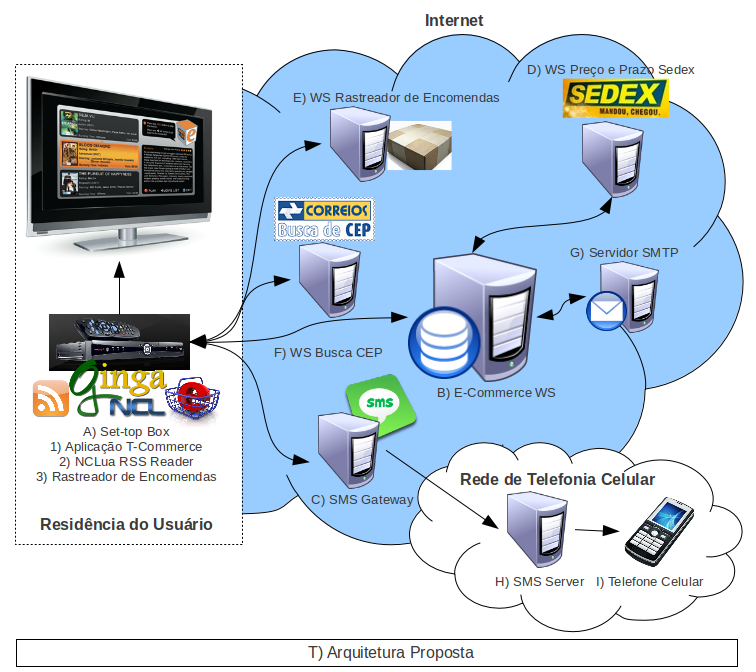
\includegraphics[width=0.8\textwidth]{TCommerce-Arquitetura.png}
	\captionof{figure}{Visão Geral da Arquitetura SOA proposta para \textit{T-Commerce}}
	\label{fig:arquitetura-tcommerce}
\end{center}

\subsubsection*{A) Conversor Digital/\textit{Set-top Box} (STB)\nomenclature{STB}{\textit{Set-top Box} (Conversor Digital)}}
Conversor digital, televisor com conversor integrado contendo o \textit{middleware} Ginga,
onde serão executadas as aplicações de TV Digital Interativa. Tais aplicações são conhecidas como
\textit{Thin Client} (Clientes Leves/Magros)\cite{sommerville2011soft} por apenas conterem uma camada de apresentação,
todas (ou grande parte) das regras de negócio são processadas no lado servidor.

Visando experimentos futuros, considera-se o uso de \textit{notebooks} ou telefones celulares com implementações
de Ginga-NCL para teste das aplicações desenvolvidas.

Tais equipamentos serão denominados daqui por diante como receptor/equipamento de TVD.

\subsubsection*{B) \textit{E-Commerce WS}} \label{sec:ecommercews}

\textit{Web Services} contendo as rotinas utilizadas em uma loja virtual convencional
na \textit{Internet}, que serão utilizadas pela aplicação de TV Digital para prover
comércio eletrônico pela TV. Tais \textit{Web Services} encapsulam todas as regras
de negócio para o gerencimento da loja virtual, como rotinas de cadastro de clientes,
produtos, pedidos, etc. A aplicação de TV Digital consumirá tal \textit{Web Service}
para prover muitas das funcionalidades disponíveis aos usuários.

\added{
O uso de tais \textit{Web Services} é essencial para centralizar
as regras de negócio utilizadas tanto pela aplicação de \textit{E-Commerce}
(normalmente acessada a partir de computadores ou dispositivos móveis como aparelhos celulares)
como pela aplicação de \textit{T-Commerce} (acessada a partir de receptores de TVD).
}

\subsubsection*{C) \textit{SMS Gateway}}

O \textit{Gateway} SMS\nomenclature{SMS}{\textit{Short Message Service}} é utilizado como intermediário para comunicação via SMS da loja com o cliente.
Devido à arquitetura proposta ser baseada em \textit{Web Services}, o uso do \textit{Gateway} facilita tal 
integração com a rede de telefonia celular.

Um serviço implementado na aplicação de \textit{T-Commerce} que requer o uso de SMS é a recuperação de senha, permitindo
que o usuário que esqueceu a senha, receba a mesma via mensagem SMS no telefone celular
que estiver cadastrado na loja. Tais serviços não são gratuitos e cobram por cada SMS enviado. 

O uso do \textit{Gateway} SMS é essencial por tornar transparente para a aplicação qual a operadora sendo utilizada
para enviar as mensagens SMS. Um das formas de envio de SMS é utilizando \textit{softwares} específicos para determinados
aparelhos celulares. No entanto, para automatizar tal processo seria necessário fazer a integração
com tal software por meio de alguma API, normalmente específica do \textit{software}. O uso
do \textit{Gateway} dispensa tal complexidade.

\subsubsection*{D) \textit{WS} Preço e Prazo Sedex}

Na arquitetura proposta, considerou-se que as entregas da loja
sejam feitas pela Empresa Brasileira de Correios e Telégrafos (ECT)\nomenclature{ECT}{Empresa Brasileira de Correios e Telégrafos},
denominada daqui em diante simplesmente como Correios. Desta forma, a obtenção de preços,
prazos de rastreamento das encomendas utiliza recursos dos Correios. \added{Desta forma,
o uso de um \textit{Web Service} dos Correios facilita a obtenção
de tais dados a partir de qualquer aplicação.}

\subsubsection*{E) \textit{WS} Rastreador de Encomendas}

Após o cliente ter decidido realizar a compra e finalizá-la, apesar
de já saber previamente qual a previsão para a entrega do produto,
um recurso muito utilizado é o rastreamento \textit{online} da encomenda.
Para tal funcionalidade, pelo fato de estarem sendo usados
os serviços de logística dos Correios, o rastreador
de encomendas para TV Digital realiza o rastreamento
\textit{online} de encomendas postadas por tal empresa. 

\subsubsection*{F) \textit{WS} Busca CEP}

A busca de endereço a partir de um Código de Endereçamento Postal (CEP)\nomenclature{CEP}{Código de Endereçamento Postal} 
é um requisito fundamental para
a aplicação de TVD, devido ao fato de o usuário
normalmente possuir apenas o controle remoto para entrada
de dados, utilizando o mesmo da mesma forma
como entra dados em um telefone celular.
Desta forma, a aplicação de \textit{T-Commerce} precisa
reduzir ao máximo a quantidade de dados que o usuário deve
digitar, para agilizar tal processo tedioso de entrada
de dados. Na arquitetura proposta foi utilizado um \textit{Web Service} para prover tal funcionalidade.

\subsubsection*{G) Servidor SMTP}

Como a aplicação de \textit{T-Commerce} possui recurso de recuperação de senha também por \textit{e-mail},
a arquitetura proposta inclui um servidor de \textit{Simple Mail Transfer Protocol} (SMTP).
Tal servidor é também conhecido como \textit{Mail Transfer Agent} (MTA)\nomenclature{MTA}{\textit{Mail Transfer Agent}},
que é responsável por transferir mensagens de correio eletrônico entre um computador e outro.
Por meio de tal servidor, a aplicação de TVD pode, por exemplo enviar a senha do usuário para seu \textit{e-mail}
ou confirmar a realização de uma compra.

\subsubsection*{H) SMS \textit{Server}}

Os \textit{Gateways} SMS fazem a integração com o SMS \textit{Server} de alguma(s) operadora(s)
para permitir o envio das mensagens SMS. 
Logo, o SMS \textit{Server} é o responsável direto pelo envio
das mensagens SMS pela rede de telefonia celular. Desta forma, o \textit{Gateway} apenas 
se encarrega de fazer a integração com o(s) servidor(es) de SMS, tornando tranparente para a aplicação
esta comunicação com o terminal celular do usuário.

\subsection{Casos de Uso das Funcionalidades da Arquitetura}

Para dar uma visão geral das funcionalidades providas pela arquitetura, tanto para os desenvolvedores
de aplicações de TV Digital Interativa (TVDi), quanto para os usuários finais, são apresentados os 
diagramas de casos de uso a seguir.


\begin{center}
	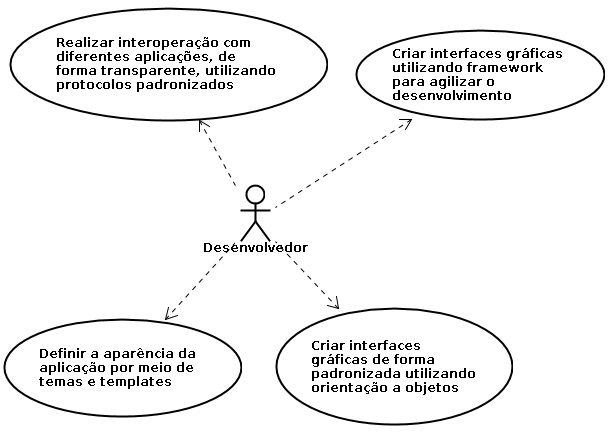
\includegraphics[width=0.7\textwidth]{TCommerce-Diagrama-Casos-de-Uso-Desenvolvedor.png}
	\captionof{figure}[Diagrama de Casos de Uso: Funcionalidades providas a desenvolvedores]{Diagrama de Casos de Uso das Funcionalidades providas a desenvolvedores de aplicações TVDi}
	\label{fig:use-case-developer}
\end{center}

A Figura \ref{fig:use-case-developer} apresenta as funcionalidades que a arquitetura provê aos desenvolvedores
de aplicações de TVDi, por meio dos \textit{frameworks} utilizados. Tais funcionalidades permitem
um grande aumento de produtividade no desenvolvimento de tais aplicações, reduzindo a quantidade
de código que os desenvolvedores precisam escrever e, consequentemente, o total de \textit{bugs}\footnote{Erro no funcionamento de um \textit{software}}.

\begin{center}
	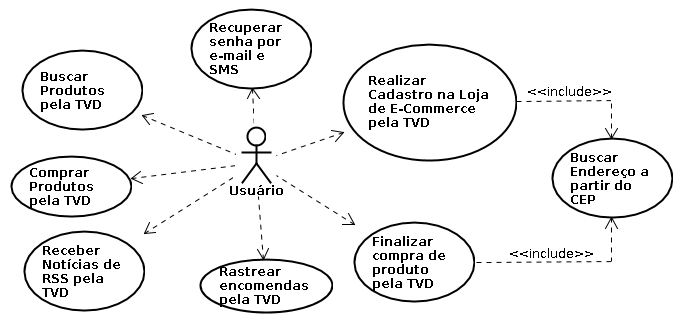
\includegraphics[width=0.7\textwidth]{TCommerce-Diagrama-Casos-de-Uso-Usuario.png}
	\captionof{figure}[Diagrama de Casos de Uso: Funcionalidades providas aos usuários]{Diagrama de Casos de Uso das Funcionalidades providas aos usuários das aplicações de TVDi desenvolvidas}
	\label{fig:use-case-usuario}
\end{center}

A Figura \ref{fig:use-case-usuario} apresenta as funcionalidades que a arquitetura provê aos usuários
de aplicações de TVDi. As funcionalidades implementadas são as consideradas mais comuns em sistemas
de \textit{E-Commerce} tradicionais.

\subsection{Tecnologias \textit{Core} da Arquitetura Proposta}

Em \cite{chu2007evolution} são tratadas as tecnologias \textit{core} para o provimento de comércio eletrônico,
divididas em quatro camadas: comunicação, apresentação e representação de informações, linguagens,
e armazenamento e recuperação de dados.

A camada de comunicação conta com as tecnologias necessárias para estabelecer a comunicação
entre as partes envolvidas nos sistemas de comércio eletrônico, assim como 
os protocolos utilizados para garantir a interoperabilidade entre as aplicações
que compõem tais sistemas. Utilizam-se, na arquitetura aqui proposta, as tecnologias
\textit{Hyper Text Transfer Protocol} (HTTP), \textit{Simple Object Access Protocol} (SOAP),
\textit{Simple Mail Transfer Protocol} (SMTP) e \textit{Short Message Service} (SMS).

A camada de apresentação e representação de informações contém as tecnologias
que definem o formato das informações, utilizado tanto para apresentação 
como para garantir a troca de informações entre sistemas heterogênos. 
Utilizam-se, na arquitetura aqui proposta, as tecnologias
\textit{eXtensible Markup Language} (XML), \textit{Really Simple Syndication} (RSS),
Lua, e imagens \textit{Joint Photographic Experts Group} (JPEG) e \textit{Portable Network Graphics} (PNG).

As linguagens de programação são utilizadas para a construção 
das regras de negócio das aplicações, definindo toda
a lógica das rotinas a serem executadas por elas.
São utilizadas as linguagens Java, \textit{Nested Context Language} (NCL) e Lua.

A camada de armazenamento e recuperação de dados
é responsável pelo armazenamento local ou remoto dos dados
das aplicações, como Sistemas Gerenciadores de Bancos de Dados (SGBD's).
São utilizadas as tecnologias MySQL \textit{DataBase Management System}, 
\textit{Java Database Connectivity} (JDBC) e \textit{Structured Query Language} (SQL).

\begin{center}
	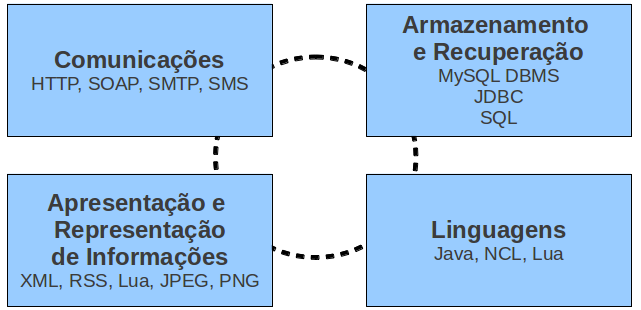
\includegraphics[width=0.8\textwidth]{TCommerce-Arquitetura-CoreTech.png}
	\captionof{figure}[Tecnologias \textit{Core} da arquitetura de \textit{T-Commerce}]{Tecnologias \textit{Core} da arquitetura de \textit{T-Commerce} (adaptada de \cite{chu2007evolution}).}
	\label{fig:tcommerce-core-tech}
\end{center}

A Figura \ref{fig:tcommerce-core-tech} apresenta as tecnologias empregadas na arquitetura proposta,
em cada uma das camadas supracitadas.


\section{Descrição dos Componentes de \textit{Software} da Arquitetura}

Conforme a Figura \ref{fig:arquitetura-tcommerce} exibida anteriormente,
nesta seção são apresentados os \textit{softwares} aplicativos que compõem
a arquitetura.

\subsection*{A) \textit{Set-top Box}}

\subsubsection*{A.1) Aplicação de \textit{T-Commerce}}

A aplicação é a interface gráfica pela qual o usuário pode realizar
compras por meio da TV Digital.

Os requisitos funcionais da aplicação foram baseados em avaliação
empírica das funcionalidades existentes na maioria dos sistemas de \textit{E-Commerce}
disponíveis no Brasil e amplamente conhecidos e utilizados.
A Tabela \ref{tab:app-tcommerce-requisitos} apresenta os requisitos funcionais e não funcionais atendidas pela aplicação.

\begin{center}
\scriptsize {
	\begin{tabular}{|p{11cm}|c|c|}
		\hline 
  		\textbf{Requisito} & \textbf{Funcional} & \textbf{Não Funcional} \\
		\hline
	  	A.1-01) Permitir a exibição de produtos em destaque ao iniciar a aplicação &  X &    \\
		\hline
		  A.1-02) Realizar a busca de produtos pelo título parcial &  X &    \\
		\hline
		  A.1-03) Adicionar produtos ao carrinho de compras &  X &    \\
		\hline
		  A.1-04) Remover produtos do carrinho de compras &  X &    \\
		\hline
		  A.1-05) Cadastrar vários endereços, permitindo ao usuário escolher um endereço
		   de entrega a partir da lista de endereços cadastrados &  X &    \\
		\hline
		  A.1-06) Permitir múltiplas formas de pagamento, possibilitando ao usuário selecionar uma das formas
		   suportadas &  X &    \\
		\hline
		  A.1-07) Cadastrar usuário &  X &    \\
		\hline
		  A.1-08) Realizar login de usuário utilizando \textit{e-mail} ou CPF &  X &    \\
		\hline
		  A.1-09) Buscar endereço a partir do CEP &  X &    \\
		\hline
		  A.1-10) Recuperar senha por \textit{e-mail} e SMS &  X &    \\
		\hline
		  A.1-11) Rastrear automatizadamente encomendas postadas pelos Correios,
		   exibindo ao usuário informações sempre que a situação
		   da encomenda mudar &  X &    \\
		\hline
		  A.1-12) Exibir preço e prazo de entrega, baseado em \textit{Web Services} dos Correios &  X &    \\
		\hline
		  A.1-13) Realizar processo de compra em etapas, permitindo que o usuário volte a uma etapa anterior,
		   antes de finalizar a compra, para alterar algum dado (como mudar a forma de pagamento) &  X &    \\
		\hline
		  A.1-14) Utilizar botões coloridos do controle remoto para o acionamento da maioria
		   das funções da aplicação &  X &    \\
		\hline
		  A.1-15) Processar grande parte das regras de negócio nos servidores \textit{Web} que integram a arquitetura,
		   desonerando o conversor digital da maior parte da carga de processamento, considerando
		   que o mesmo é um dispositivo de recursos restritos &   & X   \\
		\hline
		  A.1-16) Armazenar dos dados do carrinho de compras em memória RAM até a finalização da compra,
		   quando estes dados são enviados ao \textit{Web Service} para registro da mesma &   & X   \\
		\hline
		  A.1-17) Carregar dinâmicamente a lista de produtos a partir do \textit{Web Service} &   & X   \\
		\hline
		  A.1-18) Permitir a exibição de comunicados, ofertas de produtos e promoções & X &    \\
		\hline
	\end{tabular}
	\captionof{table}{Requisitos funcionais e não funcionais da aplicação de \textit{T-Commerce}}
	\label{tab:app-tcommerce-requisitos}
}
\end{center}

A aplicação é apenas um cliente que consome os \textit{Web Services} utilizados na arquitetura.
Assim, a maior parte da carga de processamento e regras de negócio é feita nos 
servidores \textit{Web} que hospedam os serviços. Quase todas as telas da aplicação
(que podemos chamar também de formulários ou páginas) fazem acesso a algum \textit{Web Service}
para obtenção ou registro de dados. Desta forma, a aplicação é totalmente dependente
de um canal de interatividade (também conhecido como canal de retorno)
para conexão à \textit{Internet} e acesso aos servidores \textit{Web} que hospedam os serviços.

Como o telespectador pode visualizar e comprar qualquer produto existente na loja,
e não somente aqueles que estejam em destaque, para a exibição dos produtos
sempre é feita uma consulta ao \textit{Web Service} de \textit{E-Commerce} da loja.
Em outros modelos de aplicação, como o apresentado em \cite{extra-vendas-tvd},
que exibem apenas os produtos em destaque, o telespectador não precisa
ter a TV conectada à \textit{Internet}, pois ele só visualiza os produtos 
enviados pela emissora, e não pode finalizar o processo de compra
pela TV. Desta forma, não há necessidade de conexão com a \textit{Internet}.
A arquitetura proposta vai além deste modelo, permitindo que o usuário possa comprar
qualquer produto e finalizar a compra direto da TV, o que exige a existência de um canal 
de interatividade.

A interface gráfica da aplicação foi desenvolvida
utilizando-se uma nova versão do \textit{framework} LuaOnTV\cite{junior2009luacomp}, cujas melhorias foram
desenvolvidas no presente trabalho de dissertação e são apresentadas em detalhes no Capítulo \ref{cap:luaontv}.
O LuaOnTV é a primeira e, até o momento em que esta dissertação foi desenvolvida,
a única biblioteca de componentes NCLua para criação de interfaces gráficas
em aplicações de TV Digital para o Ginga-NCL que se tem conhecimento.

Um \textit{screenshot}\footnote{Imagem capturada de uma tela de determinada aplicação em execução} da aplicação é apresentado na Figura \ref{fig:tcommerce-app-destaques}.
Tal figura mostra a tela inicial da aplicação, com os produtos em destaque na loja virtual (definidos no banco de dados da loja).
O usuário pode localizar um produto a partir de uma palavra contida no título,
inserindo tal valor por meio do controle remoto. 
O apêndice no final da dissertação mostra \textit{screenshots} de todas as telas da aplicação.

\begin{center}
	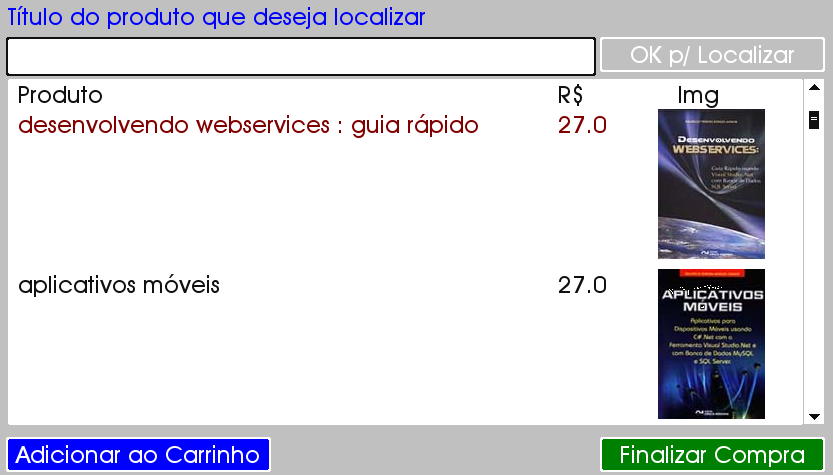
\includegraphics[width=0.8\textwidth]{CommerceApp/TCommerce-App-Destaques.png}
	\captionof{figure}{Aplicação de \textit{T-Commerce}: Tela inicial mostrando os produtos em destaque}
	\label{fig:tcommerce-app-destaques}
\end{center}

Toda a comunicação com os serviços que compõem a arquitetura é feita por meio do protocolo SOAP,
utilizando-se a implementação de SOAP para o Ginga-NCL denominada NCLua SOAP, construída
neste trabalho de dissertação e apresentada em detalhes no Capítulo \ref{cap:ncluasoap}. 

O processo de compra na aplicação de \textit{T-Commerce} desenvolvida é bastante simples e direto.
O diagrama de sequência apresentado na Figura \ref{fig:tcommerce-app-diagrama-seq-compra}
mostra como tal processo ocorre.

\begin{center}
	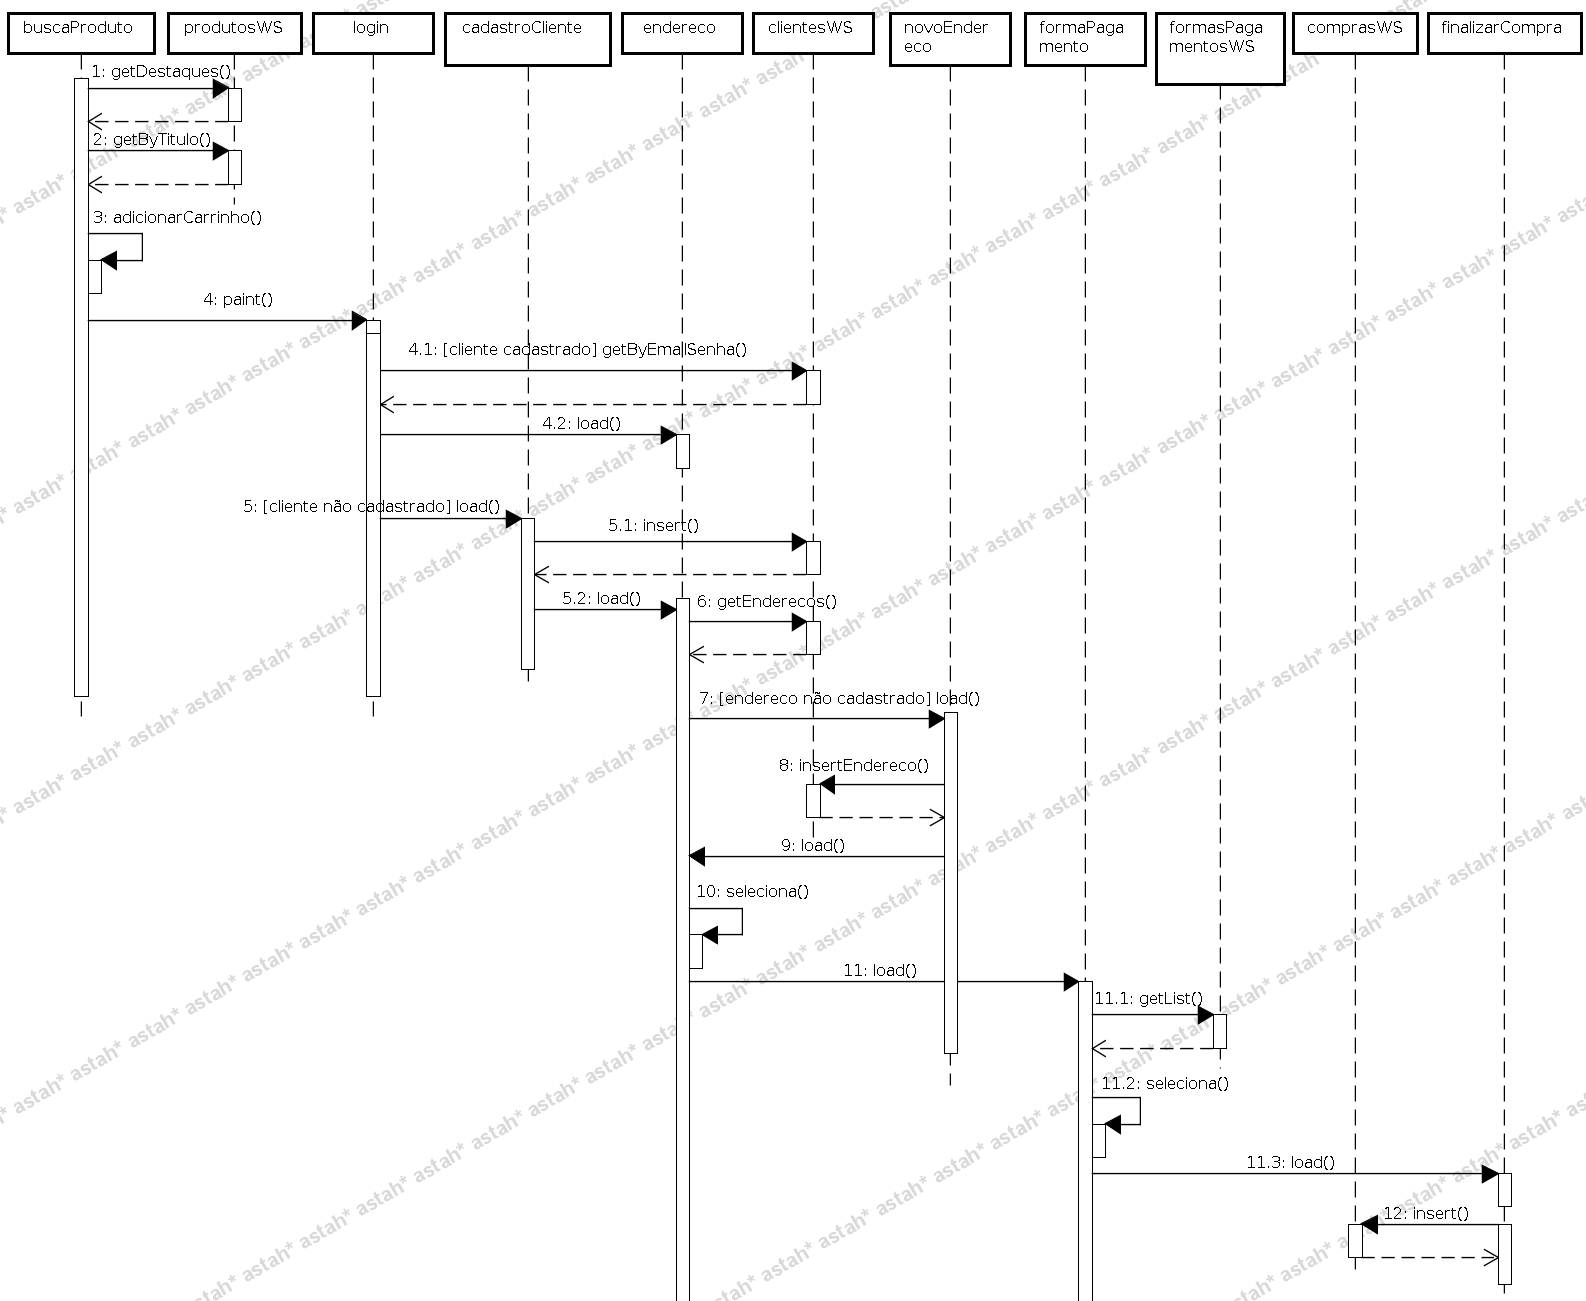
\includegraphics[width=1.2\textwidth]{TCommerce-Diagrama-Sequencia-Compra.png}
	\captionof{figure}{Aplicação de \textit{T-Commerce}: Diagrama de sequência do processo de compra}
	\label{fig:tcommerce-app-diagrama-seq-compra}
\end{center}

\subsubsection*{A.2) NCLua RSS \textit{Reader}}

Como pode ser visto na Figura \ref{fig:arquitetura-tcommerce}, o \textit{Set-top Box} 
(TV, notebook ou celular com o \textit{middleware} Ginga)
armazena a aplicação de \textit{T-Commerce} além de um leitor de RSS 
\nomenclature{RSS}{\textit{Really Simple Syndication}}desenvolvidos com as linguagens NCL e Lua.

Um arquivo RSS possui um formato XML e é utilizado para divulgação de notícias na \textit{Internet},
permitindo aos usuários assinarem os chamados \textit{feeds} RSS para
obterem as notícias de um determinado provedor desejado.
Os \textit{feeds} são os arquivos RSS que contêm as notícias em formato XML.
Com o RSS, a notícia vai até o usuário, no lugar de ele ir até a notícia.
Assim, tendo um leitor de RSS, o usuário pode adicionar vários \textit{feeds}
e receber várias notícias de diferentes provedores.

O leitor de RSS implementado para a TV Digital nesta dissertação é denominado 
\textit{NCLua RSS Reader}\footnote{\url{http://ncluarss.manoelcampos.com} e \url{http://labtvdi.unb.br}}.
Ele implementa o padrão RSS 2.0\cite{rss2} 
e compõe a arquitetura de \textit{T-Commerce} para permitir que, quando
o usuário não estiver acessando a aplicação da loja virtual pela TV, ele
possa ficar atualizado com as promoções que a loja esteja divulgando.

A aplicação utiliza o módulo LuaXML\footnote{\url{http://lua-users.org/wiki/LuaXml}} 
(que foi estendido para funcionar com Lua 5). Este é um parser XML escrito completamente
em Lua, que permite obter as notícias do \textit{feed} RSS e exibir em um equipamento de TVD.
A aplicação utiliza o módulo NCLua HTTP para fazer o \textit{download} do 
arquivo RSS diretamente do site do provedor de conteúdo, neste caso
o servidor \textit{Web} da loja virtual. O NCLua HTTP será apresentado no Capítulo \ref{cap:ncluasoap}.
O \textit{NCLua RSS Reader} ainda utiliza o módulo \textit{canvas} de NCLua para desenho 
da interface gráfica, além do módulo \textit{event} para tratamento de eventos.

A Figura \ref{fig:ncluarssreader} apresenta um \textit{screenshot} da aplicação de leitura de RSS em execução,
mostrando a mesma sendo exibida sobre o vídeo principal da emissora (em um ambiente
simulado, o \textit{Ginga Virtual Set-top Box}).

\begin{center}
	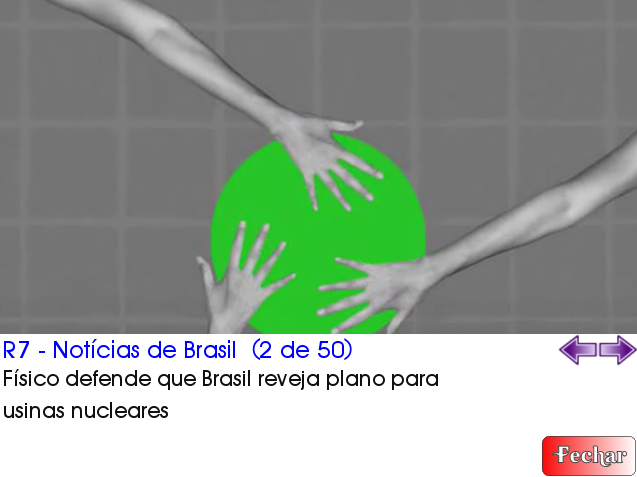
\includegraphics[width=1.00\textwidth]{nclua-rss-reader.png}
	\captionof{figure}{\textit{NCLua RSS Reader} - Leitor de Notícias para TV Digital}
	\label{fig:ncluarssreader}
\end{center}

\subsubsection*{A.3) Rastreador de Encomendas para TVD}

O rastreador de encomendas para a TV Digital faz acesso a este \textit{Web Service} desenvolvido
para o Ginga-NCL, utilizando as linguagens NCL e Lua e o módulo NCLua SOAP, este a ser apresentado no Capítulo \ref{cap:ncluasoap}.

As Figuras \ref{fig:rastreador-encomendas-tvd1} e \ref{fig:rastreador-encomendas-tvd2} apresentam \textit{screenshots} da aplicação em execução.
Tal aplicação, juntamente com o módulo NCLua SOAP, foi ganhadora do Concurso Latino-Americano de Conteúdo para TV Digital Interativa
\footnote{\url{http://clube.ncl.org.br/node/82}},
na categoria \textit{Widgets}, realizado pela PUC-Rio em 2010.

\begin{center}
	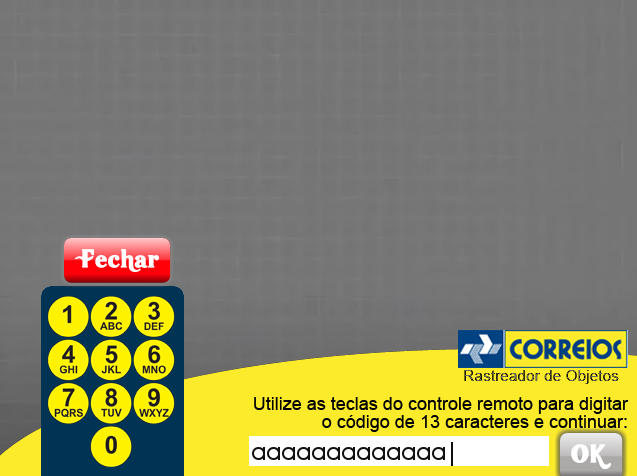
\includegraphics[width=0.9\textwidth]{rastreador/rastreador1.png}
	\captionof{figure}{Rastreamento de encomendas pela TVD: Inserção do código de rastreamento}
	\label{fig:rastreador-encomendas-tvd1}
\end{center}

\begin{center}
	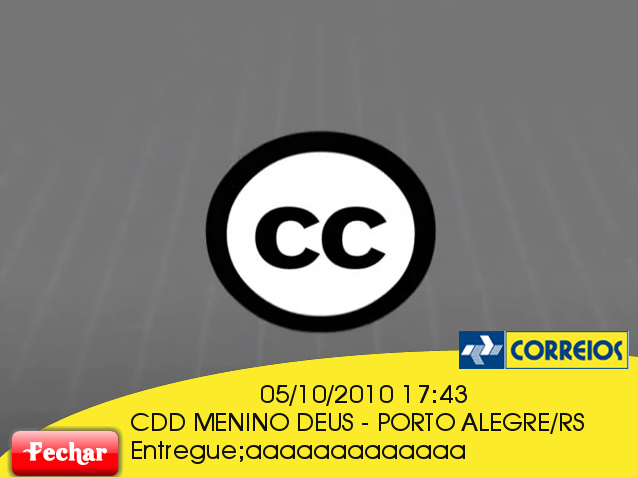
\includegraphics[width=0.9\textwidth]{rastreador/rastreador2.png}
	\captionof{figure}[Rastreamento de encomendas pela TVD: Situação da entrega da encomenda]{Rastreamento de encomendas pela TVD: Situação da entrega da encomenda (atualizada automaticamente a cada 5 minutos)}
	\label{fig:rastreador-encomendas-tvd2}
\end{center}

\subsection*{B) \textit{E-Commerce WS}}

O \textit{E-Commerce WS} contém um conjunto de \textit{Web Services} desenvolvidos utilizando-se o IDE NetBeans 6.7.1 e a  \textit{Java API for XML Web Services} (JAX-WS)
\nomenclature{JAX}{Java API \textit{for} XML}
\nomenclature{JAX-WS}{Java API \textit{for} XML \textit{Web Services}}
com o servidor de aplicações \textit{Glass Fish} 2.1 para execução dos \textit{Web Services}.
Tais ferramentas foram escolhidas por serem livres e multiplataforma,
amplamente utilizadas no mercado para o desenvolvimento de aplicações,
e pela familiaridade com as mesmas. O servidor de aplicações pode
ser qualquer outro (como \textit{Tomcat, Jetty ou JBoss}) que implemente a especificação de \textit{Servlet} 2.5.
Um \textit{Servlet} é uma classe Java \textit{server side}, ou seja, que executa
do lado do servidor \textit{Web}, sendo capaz de responder a requisições
HTTP com resposta em formato (X)HTML, XML e outros.
A escolha pelo \textit{Glass Fish} veio devido ao fato de ele ser a atual implementação
de referência para a plataforma \textit{Java Enterprise Edition} (Java EE)\nomenclature{Java EE}{\textit{Java Enterprise Edition}}, que provê as
tecnologias para desenvolvimento de aplicações \textit{Web} em Java.

Os métodos desenvolvidos em cada \textit{Web Service} foram implementados, baseado em um levantamento de requisitos
do que deve ter uma loja virtual, como já apresentado na Tabela \ref{tab:app-tcommerce-requisitos}. 
Utilizou-se a linguagem UML para modelar as classes e métodos
que comporiam os serviços.

A Figura \ref{fig:tcommerce-ws} apresenta um diagrama de classes com os \textit{Web Services}
implementados e seus respectivos métodos.

\begin{center}
	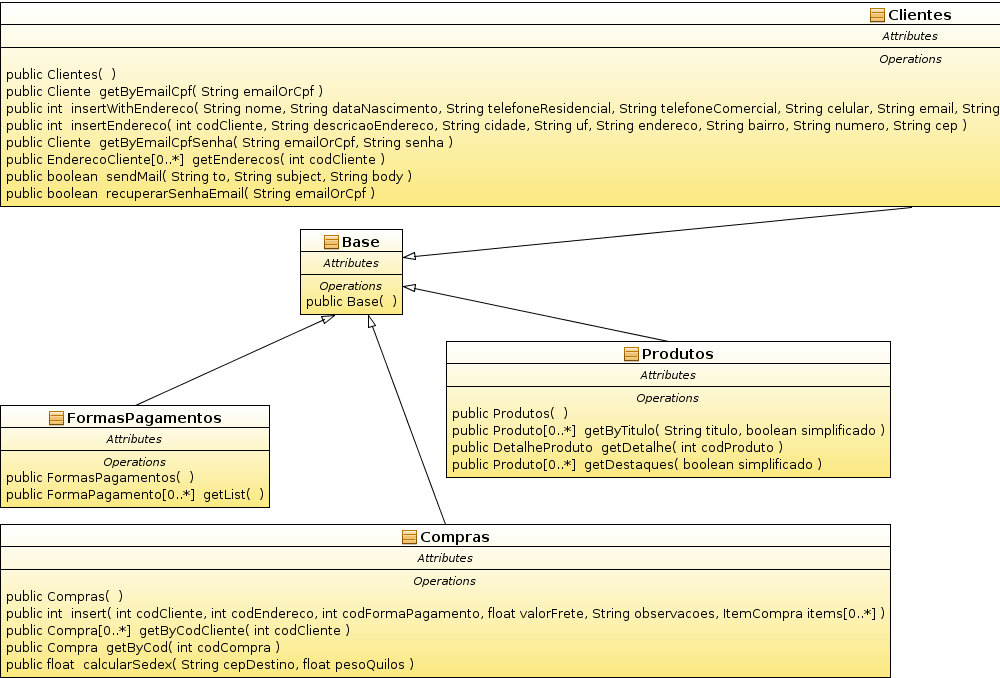
\includegraphics[width=1.00\textwidth]{TCommerce-ClassDiagramServices.png}
	\captionof{figure}{Diagrama de Classes dos \textit{Web Services} implementados}
	\label{fig:tcommerce-ws}
\end{center}

Cada \textit{Web Service} agrupa funcionalidades comuns. O "Clientes", por exemplo,
provê todas as funcionalidades para gerenciamento do cadastro do cliente, o "Compras",
todo o processo de compra, o "Produtos", todo o cadastro de produtos.

Estes \textit{Web Services} publicam os métodos a serem acessados pela aplicação de \textit{T-Commerce}.
Os mesmos são responsáveis pelo gerenciamento de todos os dados armazenados pela loja (como produtos, clientes
e pedidos de compra). Eles utilizam as classes Java apresentadas na Figura \ref{fig:tcommerce-ws-classes}
como base para seus métodos.

Tais classes são responsáveis pelo gerenciamento do cadastro do cliente, cadastro de produtos,
formas de pagamento, compras e tipo de frete. Para o armazenamento destes
dados foi utilizado o Sistema Gerenciador de Banco de Dados (SGBD) \textit{MySQL 5.1}
por ser um sistema multiplataforma, livre, bastante leve, que não requer
muitos recursos de hardware e amplamente utilizado no mercado, além
da familiaridade com o mesmo. No entanto, a arquitetura pode utilizar qualquer outro
banco de dados que for desejado, pois o acesso aos dados
é feito por meio da API \textit{Java Database Connectivity} (JDBC)\nomenclature{JDBC}{\textit{Java Database Connectivity}}
que é compatível com diversos SGBD's existentes no mercado. Além disto,
foi utilizado o padrão de projeto \textit{Data Access Objects} (DAO)\nomenclature{DAO}{\textit{Data Access Objects}}
que permite fazer uma separação total entre as classes de negócio e as instruções
SQL para acesso ao banco de dados.

\begin{center}
	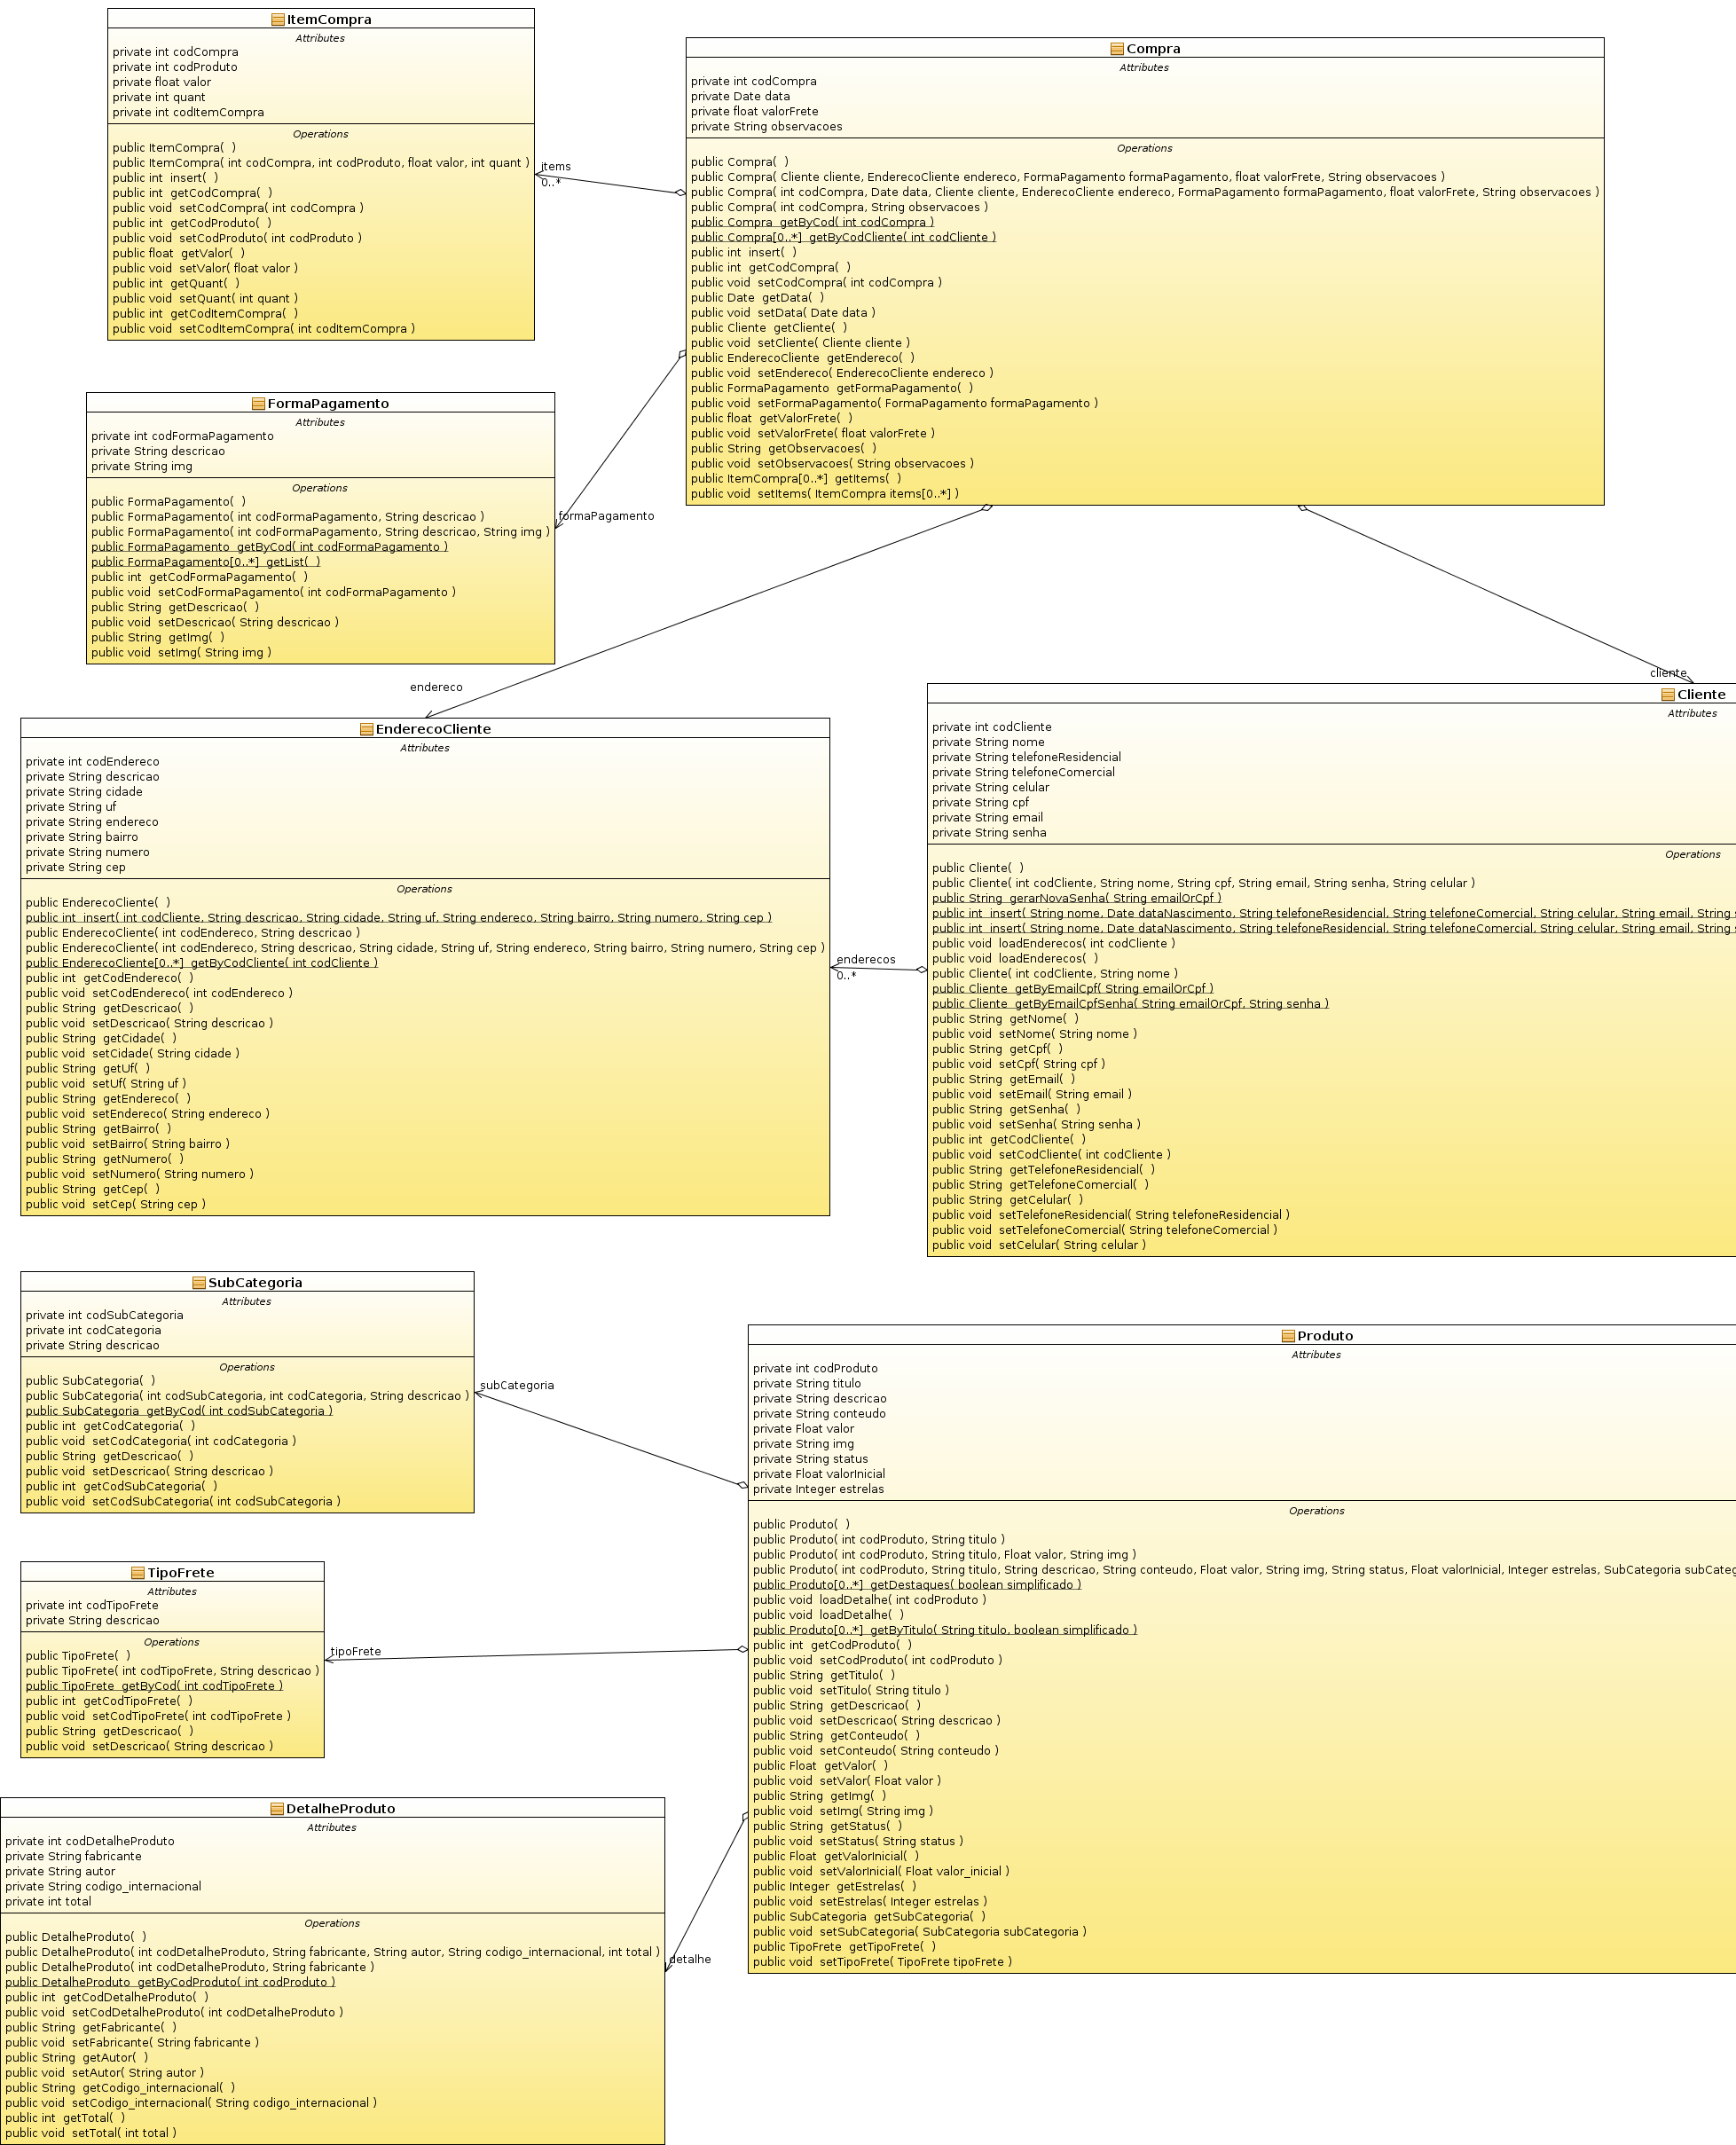
\includegraphics[scale=0.25]{TCommerce-ClassDiagramModel.png}
	\captionof{figure}{Diagrama das classes utilizadas internamente pelos WS's implementados}
	\label{fig:tcommerce-ws-classes}
\end{center}


Os \textit{Web Services} não utilizam nenhum \textit{framework} de persistência por falta
de familiaridade com tais tecnologias e restrições de tempo. No entanto,
a utilização de algum \textit{framework} como \textit{Hibernate} ou \textit{Java Persistent API} (JPA)\nomenclature{JPA}{\textit{Java Persistent API}}
não altera em nada a comunicação entre a aplicação de TVD e os \textit{Web Services}.
Tal mudança arquitetural pode ser feita para aumentar o nível de abstração
do acesso ao banco de dados e automatizar a geração das instruções
SQL\nomenclature{SQL}{\textit{Structured Query Language}} necessárias para isto, sob pena de aumentar o \textit{overhead} de acesso aos dados.

\subsection*{C) \textit{SMS Gateway}}

Para a arquitetura proposta, foi utilizado o \textit{Gateway} MyTalk\footnote{\url{http://www.mytalk.com.br}},
que permite o acesso via \textit{Web Services} SOAP. Contudo, tal componente
pode ser substituído na arquitetura por qualquer outro \textit{Gateway} SMS.
Todos os \textit{gateways} encontrados e testados, disponibilizam acesso via SOAP ou REST.
A escolha de tal serviço foi feita por ter sido o primeiro encontrado,
mas reitera-se que qualquer outro pode ser utilizado, levando-se em consideração
custo, resiliência, QoS (como tempo de resposta), etc.

Caso o usuário esqueça sua senha, ele pode informar seu \textit{e-mail} ou CPF na aplicação 
de TVD e recuperá-la via \textit{e-mail} ou SMS. Como ele normalmente estará na frente da TV, sair
deste local para ir até um computador e entrar no seu \textit{e-mail} para pegar 
uma nova senha é bastante incômodo. Como o celular é algo pessoal e
que geralmente as pessoas o mantêm por perto o tempo todo, o usuário
pode receber a nova senha sem precisar sair da frente da TV,
facilitando o processo de compra.

Neste caso, optou-se por a aplicação de TV enviar a requisição diretamente
ao \textit{Gateway} SMS, no lugar de requisitar ao \textit{Web Service} da loja (\textit{E-Commerce} WS)
para depois este despachar a requisição ao \textit{Gateway} SMS, 
no intuito de reduzir o tempo de resposta para a aplicação de \textit{T-Commerce}.
No entanto, esta abordagem tem a desvantagem de vincular a aplicação
a um determinado \textit{Gateway} SMS. Caso escolha-se utilizar
um \textit{Gateway} diferente, a aplicação precisará ser atualizada.
Centralizando tal regra de negócio no \textit{Web Service} da loja, não haverá
tal problema, mas aumentará o tempo de resposta da requisição
que precisará ser encaminhada ao \textit{Gateway}.

\subsection*{D) \textit{WS} Preço e Prazo Sedex}

Um dos recursos básicos que toda loja virtual deve prover a seus usuários é 
informar o preço e prazo para entrega do produto. Tals informações
podem ser decisivas para a concretização ou não da compra.

Os Correios são responsáveis por grande parte das entregas de produtos e correspondências em todo o país.
Desta forma, a arquitetura de \textit{T-Commerce} proposta faz integração com 
o \textit{Web Service} dos Correios\footnote{\url{http://www.correios.com.br/webservices/}} que permite calcular o preço e prazo de entrega
de uma correspondência/produto de/para qualquer lugar do país.
Logo, a aplicação de \textit{T-Commerce} consegue exibir o preço e prazo para entrega do(s) produto(s)
que o usuário deseja comprar, acessando tal \textit{Web Service}.

A atual versão da proposta permite apenas calcular preço e prazo de entrega de encomendas
utilizando o serviço de entregas rápidas dos Correios, denominado Sedex, mas
a obtenção de informações de entrega para outros serviços dos Correios
pode ser feita facilmente a partir da implementação atual.

A Figura \ref{fig:tcommerce-app-ws-correios} apresenta quais informações
podem ser obtidas do \textit{Web Service} dos Correios. 

\begin{center}
	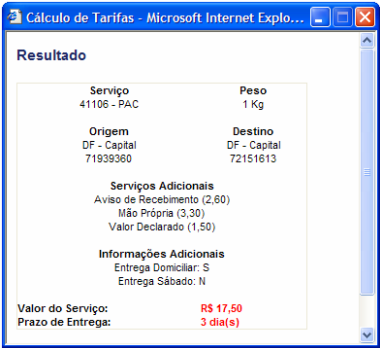
\includegraphics[width=0.8\textwidth]{TCommerce-PrecoPrazoSedex.png}
	\captionof{figure}[\textit{Web Service} dos Correios: Calculando preço e prazo de entrega de encomenda]{\textit{Web Service} dos Correios: Calculando preço e prazo de entrega de encomenda (fonte: \url{http://www.correios.com.br/webservices/}).}
	\label{fig:tcommerce-app-ws-correios}
\end{center}


O acesso ao serviço é feito a partir do \textit{E-Commerce WS} apresentado na Seção \ref{sec:ecommercews}.
Assim, a aplicação de \textit{T-Commerce} em NCLua envia uma requisição ao \textit{Web Service} "Compras"
que possui o método "calcularSedex" que retorna as informações sobre preço e prazo de entrega,
como apresentado no diagrama de classes da Figura \ref{fig:tcommerce-ws}.


\subsection*{E) \textit{WS} Rastreador de Encomendas}

Os Correios possuem um serviço na \textit{Internet} que permite ao usuário
saber a situação da entrega de uma determinada encomenda,
a partir do código de rastreamento da mesma.

No entanto, o usuário, para ficar atualizado da situação,
precisa periodicamente acessar tal página, gastando
tempo que ele poderia utilizar em outras atividades
mais importantes.

Assim, na arquitetura proposta, decidiu-se implementar um
serviço automatizado para rastreamento de encomendas,
onde o usuário possa acessar o serviço e deixar a tela
do mesmo aberta, sem precisar interagir com ela ou ficar voltando
lá para verificar se a situação da encomenda mudou.
Uma vez tendo aberta a tela do serviço, o usuário será
automaticamente notificado por meio de uma mensagem sonora,
que a situação da encomenda mudou.

O serviço está disponível via \textit{Web}\footnote{\url{http://rastreador.manoelcampos.com} e \url{http://labtvdi.unb.br}}
e foi também implementado em uma aplicação de TV Digital para o Ginga-NCL.

Como os Correios não disponibilizam
tal serviço de rastreamento por meio de um \textit{Web Service}, 
para facilitar a integração do serviço em diferentes arquiteturas, foi desenvolvido
um \textit{Web Service} para o rastreador. 
Este é responsável por fazer o \textit{parse} do código HTML da página do serviço dos Correios
e obter as informações sobre o rastreamento da encomenda. Tais informações
são extraídas e retornadas pelo \textit{Web Service} de forma estruturada, permitindo
a exibição delas facilmente em qualquer aplicação em diferentes plataformas.
Um exemplo é a aplicação iComenda\footnote{\url{http://itunes.apple.com/br/app/icomenda/id412358490?mt=8}}, 
desenvolvida por Maurício Júnior\footnote{\url{http://mauriciojunior.org}}, para os dispositivos
móveis iPhone, iPod e iPad, a partir do \textit{Web Service} disponibilizado.

\subsection*{F) \textit{WS} Busca CEP}

Infelizmente os Correios não disponibilizam um \textit{Web Service}
para a consulta de endereços a partir de um número de CEP.
Só há disponível uma página \textit{Web} para usuários finais\footnote{\url{http://www.buscacep.correios.com.br}}
que retorna os dados do endereço como uma imagem, para impedir (ou pelo menos dificultar bastante) 
que aplicações consigam acessar a página e extrair tais dados. Tal atitude provavelmente
é devida ao fato de os Correios terem um \textit{software} comercial, denominado
Guia Postal Brasileiro Eletrônico\footnote{\url{http://www.correios.com.br/servicos/cep/gpbe.cfm}}, 
contendo um banco de dados de CEP's, que é vendido na sua loja virtual e nas agências.

No entanto, existem alguns \textit{Web Services} de terceiros
que permitem obter o endereço a partir de um CEP. Qualquer
um deste serviços pode ser utilizado na arquitetura implementada
para permitir a obtenção de endereços.

Para a implementação realizada, foi escolhido o \textit{Web Service} disponível em 
\url{http://www.maniezo.com.br/webservice/soap-server.php}, por ter sido o primeiro
a ser encontrado. Tal serviço requer a realização de um cadastro prévio 
para poder acessá-lo, e com os poucos testes realizados, retornou os endereços
corretos e atualizados.

A aplicação de \textit{T-Commerce} faz acesso direto a tal serviço para obter um endereço,
utilizando-se o módulo NCLua SOAP.

\subsection*{G) Servidor SMTP}

Para envio de \textit{e-mail}, a aplicação de \textit{T-Commerce} acessa o método \textit{sendMail} do \textit{Web Service} "Clientes" do \textit{E-Commerce WS}, apresentado na Seção \ref{sec:ecommercews} e na Figura \ref{fig:tcommerce-ws}, para 
enviar \textit{e-mail} ao cliente. Desta forma, a aplicação cliente não acessa diretamente
o servidor de \textit{e-mail}. O \textit{E-Commerce WS} é que faz esta integração, despachando
a requisição para o servidor SMTP.

O \textit{E-Commerce WS} utiliza a API Java \textit{Mail}, funcionando como um cliente SMTP para
despachar a mensagem de \textit{e-mail}. Ele torna transparente para a aplicação, o servidor
de \textit{e-mail} utilizado e as configurações para acesso ao mesmo.

Na implementação feita, foi utilizado um servidor de \textit{e-mail} disponibilizado por um plano de hospedagem
profissional, logo é um serviço com custo mensal. No entanto, pode-se utilizar qualquer servidor de \textit{e-mail} que desejar,
como por exemplo um que seja disponibilizado por serviços de \textit{WebMail} gratuitos, amplamente
difundidos na \textit{Internet} e usados no cotidiano. 

\section{Diagrama de Distribuição/Implantação}

A Figura \ref{fig:diag-distribuicao} apresenta um diagrama de distribuição/implantação
que mostra como os componentes da arquitetura, apresentados na Seção \ref{sec:apresentacao-arquitetura} 
são distribuídos em diversos \textit{hardwares},
mostrando a arquitetura distribuída montada e a relação de dependência entre cada componente.
Tal diagrama apresenta todos os componentes de \textit{hardware} e \textit{software} da arquitetura proposta,
incluindo os \textit{softwares} aplicativos e os \textit{frameworks} implementados.

\begin{center}
	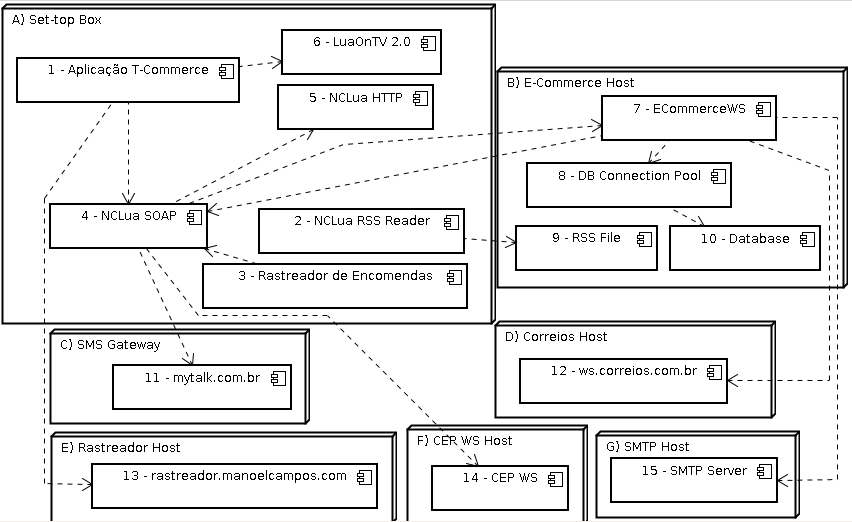
\includegraphics[width=1.00\textwidth]{TCommerce-Diagrama-Distribuicao.png}
	\captionof{figure}{Arquitetura de \textit{T-Commerce}: Diagrama de Distribuição/Implantação}
	\label{fig:diag-distribuicao}
\end{center}

As funcionalidades de cada componente são resumidas a seguir:

\begin{enumerate}[A)]
	\item \textit{Set-top Box} - Conversor de TV Digital, TV com conversor integrado, notebook ou celular que executa as aplicações de TVD desenvolvidas:
	\begin{itemize}
		\item 1 - Aplicação \textit{T-Commerce}: aplicação de comércio eletrônico para TVD (aplicação cliente);
		\item 2 - \textit{NCLua RSS Reader}: leitor de notícias para TVD, utilizado para ver notícias e ofertas de produtos;
		      da loja virtual;
		\item 3 - Rastreador de Encomendas para TVD: permite ao usuário rastrear a entrega do(s) produto(s) comprado(s) por meio da TV Digital,
		sendo notificado sempre que a situação da encomenda mudar;
		\item 4 - NCLua SOAP: módulo para acesso a \textit{Web Services} SOAP em aplicações NCLua para TVD;
		\item 5 - NCLua HTTP: módulo que implementa o protocolo HTTP, utilizado pelo NCLua SOAP e por aplicações
		          como o \textit{NCLua RSS Reader}. O módulo é apresentado no Capítulo \ref{cap:ncluasoap};
		\item 6 - LuaOnTV 2.0: \textit{framework} para construção da interface gráfica da aplicação de \textit{T-Commerce}.
	\end{itemize}
	\item \textit{E-Commerce Host} - Servidor \textit{Web} que hospeda os \textit{Web Services} a serem utilizados pela aplicação de \textit{T-Commerce}:
	\begin{itemize}
		\item 7 - \textit{ECommerceWS}: \textit{Web Services} da loja virtual, implementados em Java com a API JAX-WS;
		\item 8 - \textit{DB Connection Pool}: \textit{pool} de conexões ao banco de dados, implementado utilizando a API JDBC,
		que permite que conexões ao banco de dados sejam compartilhadas entre diferentes requisição ao \textit{Web Service},
		possibilitando um aumento de performance no acesso aos dados;
		\item 9 - \textit{RSS File}: arquivo RSS contendo as notícias e ofertas de produtos a serem divulgados pela loja virtual;
		\item 10 - \textit{Database}: banco de dados \textit{MySQL Server} 5.1 que armazena todos os dados da loja virtual, como cadastro
		de clientes, produtos e pedidos de compra.
	\end{itemize}
	\item SMS \textit{Gateway} - \textit{Gateway} para envio de mensagens SMS aos clientes:
	\begin{itemize}
		\item 11 - mytalk.com.br: \textit{Host} que hospeda o serviço \textit{MyTalk} SMS, um \textit{Gateway} para envio de mensagens SMS.
	\end{itemize}
	\item Correios \textit{Host} - \textit{Host} dos correios que hospeda \textit{Web Services} como os para consulta de preço e prazo de entrega de encomendas:
	\begin{itemize}
		\item 12 - ws.correios.com.br: \textit{Web Services} dos Correios para consulta de preço e prazo de entrega de encomendas.
	\end{itemize}
	\item Rastreador \textit{Host} - \textit{Host} que armazena o serviço de rastreamento de encomendas postadas pelos Correios:
	\begin{itemize}
		\item 13 - rastreador.manoelcampos.com: \textit{Web Service} de rastreamento de encomendas.
	\end{itemize}
	\item CEP WS \textit{Host} - \textit{Host} que hospeda um dos serviços de busca de endereço a partir do CEP:
	\begin{itemize}
		\item 14 - CEP WS: \textit{Web Service} maniezo.com.br que fornece o endereço a partir de um CEP
	\end{itemize}
	\item SMTP \textit{Host} - \textit{Host} que hospeda servidor de \textit{e-mail}:
	\begin{itemize}
		\item 15 - SMTP \textit{Server}: Servidor de \textit{e-mail} para envio de mensagens eletrônicas aos clientes da loja virtual.
	\end{itemize}
	\item SMS \textit{Server} - \textit{Host} de uma operadora de telefonia celular, responsável pela comunicação via SMS com o terminal celular do usuário.
\end{enumerate}


\section{Ambiente de desenvolvimento} \label{sec:dev-env}

Para o desenvolvimento do projeto foram utilizados:

\begin{itemize}
	\item sistema operacional GNU/Linux Ubuntu 10.10 como sistema \textit{desktop} para realização das tarefas de desenvolvimento;
	\item \textit{Astah Community} 6.1 (antigo \textit{Jude}) para modelagem UML;
  \item \textit{soapUI} 3.5.1 para testes de consumo de \textit{Web Services} SOAP;
	\item IDE\nomenclature{IDE}{\textit{Integrated Development Environment}} Eclipse 3.6 para desenvolvimento de aplicação Ginga-NCL:
	\begin{itemize}
		\item \textit{plugin} NCLEclipse 1.5.1;
		\item \textit{plugin} LuaEclipse 1.3.1;
	\end{itemize}
	\item ferramenta LuaDoc\footnote{\url{http://luadoc.luaforge.net}} para geração de documentação;
	\item implementação de referência do Ginga-NCL (Ginga Virtual Set-top Box 0.11.2);
	\item interpretador Lua para execução do \textit{scripts} fora do Ginga \textit{Virtual Set-top Box};	
	\item \textit{XVidCap} 1.1.7 para captura de \textit{screencasts}\footnote{Vídeo mostrando a execução de determinada aplicação} da aplicação em execução;
	\item IDE \textit{NetBeans} 6.7.1 para modelagem UML e desenvolvimento dos \textit{Web Services} da loja virtual, 
	utilizando API JAX-WS; servidor de aplicações \textit{Glass Fish} 2.1 para execução dos 
	\textit{Web Services} da loja virtual \footnote{\url{http://java.net/projects/openesb}};
	\item \textit{Java Development Kit} (JDK)\nomenclature{JDK}{\textit{Java Development Kit}} 1.6.0.24, o kit de desenvolvimento
	Java, contendo API's e ferramentas para desenvolvimento de aplicações;
	\item \textit{Java Runtime Environment} (JRE)\nomenclature{JRE}{\textit{Java Runtime Environment}} 1.6.0.24, o ambiente
	de execução Java para execução das aplicações Java como os \textit{Web Services} criados, os IDE's e outras
	ferramentas desenvolvidas em Java como o \textit{soapUI};
	\item \textit{MySQL Server} 5.1 como Sistema Gerenciador de Banco de Dados (SGBD)\nomenclature{SGBD}{Sistema Gerenciador de Banco de Dados} para os \textit{Web Services} da loja virtual;
	\item \textit{PhpMyAdmin} para administração do banco de dados;
	\item PHP 5.3 e Apache 2 para execução do \textit{PhpMyAdmin};
	\item \textit{VirtualBox} 4.0 e \textit{RemasterSys} para criação de distribuição Linux contendo todo o ambiente de desenvolvimento, com
	todas as ferramentas apresentadas acima.
\end{itemize}

\section[Distribuição GNU/Linux p/ desenvolvimento de aplicações]{Distribuição GNU/Linux para desenvolvimento, execução e teste de aplicações de TV Digital}

Com base no trabalho apresentado em \cite{soset}, foi gerada uma distribuição GNU/Linux
contendo todo o ambiente de desenvolvimento necessário para a construção das
aplicações apresentadas ao longo deste trabalho.
O ambiente contém todas as ferramentas apresentadas em \ref{sec:dev-env}. 
Tal distribuição GNU/Linux foi
elaborada com o intuito de facilitar a montagem do ambiente de desenvolvimento
necessário para a construção de aplicações NCL/Lua para a TV Digital.

A comunidade Ginga no Portal do Software Público disponibiliza
uma implementação de referência do sub-sistema Ginga-NCL em forma
de uma máquina virtual já com tal implementação compilada e instalada. 
Tal máquina virtual facilita bastante a montagem do ambiente
de desenvolvimento, uma vez que o processo de compilação
de tal implementação é bastante extenso, dependendo de diversos
softwares e bibliotecas, não sendo um processo trivial de 
ser executado, principalmente para usuários menos
experientes com distribuições GNU/Linux e ferramentas
de compilação de linha de comando. No entanto,
o uso de uma máquina virtual adiciona um \textit{overhead} 
de tempo no processo de teste das aplicações, uma vez
que os arquivos das mesmas precisam ser enviados via SSH para a máquina
virtual, apesar de tal processo ser automatizado com o \textit{plugin} NCL Eclipse.

Desta forma, a instalação da implementação de referência do Ginga-NCL diretamente no 
sistema operacional utilizado pelo desenvolvedor para as suas tarefas rotineiras
(como envio de \textit{e-mail's}, elaboração de documentos em \textit{suites} de escritórios, etc) 
e de desenvolvimento de sistemas agiliza bastante o processo de execução e teste
das aplicações interativas, pois, como o Ginga é instalado localmente na máquina real,
não há processo de transferência de arquivos para poder executar as aplicações.
Com isto, a execução das aplicações é praticamente instantânea, além de
obter-se melhor desempenho executando o Ginga nativamente no sistema 
operacional da máquina real, uma vez que o uso de uma máquina
virtual obviamente requer o consumo de mais memória RAM e processador
que executar o Ginga nativamente em uma máquina real.

A distribuição desenvolvida foi baseada na versão 10.10 do Ubuntu e permite
o uso do ambiente de desenvolvimento sem a necessidade de instalação do mesmo
na máquina do desenvolvedor, podendo ser dado \textit{boot} na máquina por meio
de um CD contendo tal distribuição, conhecido como \textit{Live CD}. Ela pode
ser instalada em uma máquina real, onde o usuário poderá utilizar tal
distribuição como seu sistema operacional \textit{Desktop} para
a realização de suas tarefas rotineiras e de desenvolvimento e ainda
pode ser instalada em uma máquina virtual, já com o ambiente gráfico e todas
as ferramentas de desenvolvimento necessárias.

A versão da implementação de referência do Ginga-NCL embarcada na distribuição
é a última (até a data de entrega de tal dissertação), a 0.11.2 revisão 23, disponível
na Comunidade Ginga do Portal do Software Público\footnote{\url{http://svn.softwarepublico.gov.br/trac/ginga/wiki/Building\_Wiki\_GingaNCL}}.

O processo de criação da distribuição GNU/Linux consistiu basicamente em:
\begin{itemize}
	\item instalar distribuição Ubuntu 10.10 em uma máquina virtual utilizando a ferramenta Virtual Box 4.0;
	\item baixar e compilar a implementação de referência do Ginga-NCL em tal máquina virtual, juntamente
	com todas suas dependêncais;
	\item instalar ferramentas de desenvolvimento e suas dependências (como JDK e JRE);
	\item configurar ferramentas de desenvolvimento para permitir a execução local de aplicações NCL/Lua;
	\item gerar uma nova distribuição a partir do ambiente criado, já com todas as ferramentas instaladas,
	utilizando o \textit{software} \textit{RemasterSys}\footnote{\url{http://remastersys.sourceforge.net}}.
\end{itemize}

Tal distribuição pode ser \replaced{obtida}{baixada} pelo \textit{site} do Laboratório de TV Digital Interativa da Universidade de Brasília\footnote{\url{http://labtvdi.unb.br}}.




\chapter{Framework LuaOnTV 2.0} \label{cap:luaontv}
Atendendo ao requisito "T3) Facilitar o desenvolvimento de aplicações interativas"  apresentado na Seção \ref{sec:req-arquitetura},
foi utilizado o \textit{framework} LuaOnTV, como ponto de partida, no qual foram realizadas melhorias a serem apresentadas neste capítulo.

O LuaOnTV\cite{junior2009luacomp} é um \textit{framework} para facilitar o desenvolvimento de aplicações procedurais
para o Sistema Brasileiro de TV Digital, utilizando a linguagem Lua, por meio
de \textit{scripts} NCLua (\textit{scripts} Lua embutidos em documentos NCL).
O mesmo foi resultado de trabalho de projeto de pesquisa desenvolvido por equipe do Laboratório de TV Digital Interativa da
Universidade de Brasília, sob orientação do professor Paulo Roberto de Lira Gondim. 
Ele foi um projeto pioneiro para o SBTVD, desenvolvido inteiramente em linguagem Lua,
sob o paradigma de programação orientada a objetos, que disponibiliza um conjunto
de classes e componentes visuais e não visuais para o desenvolvimento
de aplicações interativas para TVD.

Os componentes do LuaOnTV utilizam os módulos \textit{canvas} e \textit{event} existentes em NCLua.
Tais módulos estendem as funcionalidades da linguagem Lua para o contexto de TV Digital.
Desta forma, o \textit{framework} está totalmente em conformidade com as normas do Ginga-NCL.
O \textit{framework} tem como principal objetivo facilitar a construção de interfaces gráficas
para aplicações interativas, disponibilizando componentes para entrada e saída de dados, 
além de automatizar o processo de controle de foco.

Os componentes visuais foram desenvolvidos com base nos componentes 
existentes em diferentes linguagens de programação e ambientes integrados de desenvolvimento (IDE's)
como \textit{NetBeans}, Eclipse, Adobe \textit{Dreamweaver}, \textit{Delphi}, \textit{Visual Studio} e outros; além de ferramentas
específicas para TV Digital como \textit{Jame Author} e \textit{Cardinal Studio}.

\cite{junior2009luacomp} compararam uma aplicação desenvolvida utilizando a NCL como linguagem principal e outra
utilizando o LuaOnTV, que tem a linguagem Lua como principal, e constataram que:

\begin{quote}
"uma aplicação com códigos NCL e imagens que simulam os componentes gráficos do LuaOnTV chegou a quase 1,5MB. A
mesma aplicação desenvolvida com LuaOnTV chegou a pouco mais de 60 KB."
\end{quote}

Eles também comentam que o \textit{framework} tem como um dos requisitos não funcionais 
a diminuição do tamanho do código das aplicações interativas, considerando
as capacidades restritas de memória e armazenamento dos conversores de TV Digital.
Tal requisito foi alcançado devido à utilização do paradigma de orientação a objetos, que
permite uma alta reutilização de código.


\section{Delimitação do Problema}

Devido à linguagem NCL ser uma linguagem apenas declarativa,
funcionando como uma linguagem de cola para diferentes tipos de mídias
(como GIF, JPEG, MPEG, PNG, XHTML, e outros, não restringindo nem prescrevendo nenhum
tipo de mídia)\cite{abnt200815606}, ela é uma linguagem de maior nível de abstração,
não decompondo o resultado em uma implementacão algorítmica\cite{barbosa2008tv}.
No entanto, tal linguagem não permite realização de tarefas específicas como
operações aritméticas, utilização direta de protocolos de comunicação como 
TCP, HTTP e SOAP, manipulação de arquivos, 
muito menos a definição de procedimentos (rotinas/funções).
Desta forma, a realização de tais tarefas só é possível por meio de uma linguagem
procedural como a linguagem Lua. 

No caso de entrada de dados, apesar do sub-sistema Ginga-NCL do \textit{middleware} Ginga especificar 
um recurso de teclado virtual a ser utilizado por aplicações NCL\cite{abnt200815606},
a implementação de referência do mesmo\cite{ginga-ncl-community} 
ainda não inclui tal recurso. 
Além disto, a manipulação de dados (armazenamento e obtenção) em documentos
NCL não é tão trivial como a inclusão de mídias como imagens e vídeos.

Em NCL é possível até mesmo definir o controle de foco entre campos
(por meio dos atributos \textit{moveLeft, moveRight, moveUp, moveDown}, da \textit{tag descriptor}\cite{abnt200815606})
permitindo que o usuário navegue de um campo a outro utilizando as setas
do controle remoto. No entanto, a definição da navegação entre os campos
é feita de forma completamente manual, e a inclusão ou remoção
de um novo campo no meio dos campos existentes requer a 
redefinição da ordem de navegação entre os mesmos, o que
pode ser um trabalho cansativo e suscetível a erros.

Os módulos de NCLua, utilizados pelo LuaOnTV, disponibilizam apenas um conjunto de funções básicas
específicas. Existem 5 módulos, como apresentados a seguir\cite{abnt200815606}:

\begin{itemize}
	\item \textbf{\textit{canvas}}: oferece uma API para desenhar primitivas gráficas e manipular imagens;
  \item \textbf{\textit{event}}: permite que aplicações NCLua comuniquem-se com o \textit{middleware} através de eventos (eventos NCL e de teclas);
  \item \textbf{\textit{settings}}: exporta uma tabela com variáveis definidas pelo autor do documento NCL e variáveis
 de ambiente reservadas em um nó \textit{"application/x-ginga-settings"};
  \item \textbf{\textit{persistent}}: exporta uma tabela com variáveis persistentes, que estão disponíveis para manipulação
    apenas por objetos procedurais.
\end{itemize}

A utilização direta das funções destes módulos requer um conhecimento mais profundo dos mesmos,
como temos provado durante a pesquisa e estudos de tais módulos, para o desenvolvimento
de aplicações. As funcionalidades de captura de teclas (providas pelo módulo \textit{event}) 
para entrada de dados alfabéticos e numéricos, da mesma forma como em um teclado de celular
(devido o controle remoto só possuir teclas numéricas) não é trivial. O controle de foco
a partir da captura do pressionamento das teclas direcionais do controle também é 
complicado e requer a inclusão de muito código. Tais dificuldades têm se provado verdade
pelos diversos relatos de usuários, como no Fórum da Comunidade Ginga no Portal do \textit{Software} Público\cite{ginga-ncl-community},
além de outros grupos de discussão acompanhados.

Com todas as dificuldades apresentadas, o LuaOnTV se mostrou ser uma solução ideal para a redução
da quantidade de código para a criação de aplicações procedurais com interface gráfica para a TVD, 
permitindo encapsular toda a complexidade envolvida na utilização direta dos módulos
de NCLua para chegar ao mesmo fim.

\section{LuaOnTV 2.0: Nova versão implementada}

Da mesma forma que todo projeto de \textit{software}, foi implementada e liberada uma primeira versão do LuaOnTV. 
Como extensão do trabalho de mestrado onde foi originado o mesmo, 
verificou-se que eram necessárias algumas melhorias e correções de alguns
bugs encontrados. Nesta seção será apresentada a versão 2.0
do LuaOnTV, que traz uma série de importantes novos recursos.

A seguir são listados os requisitos funcionais e não funcionais, inicialmente identificados e implementados.

\begin{center}
\scriptsize {
	\begin{tabular}{|p{11cm}|c|c|}%{|l|l|l|}
    \hline
		\textbf{Requisito} & \textbf{Funcional} & \textbf{Não Funcional} \\
    \hline
		A.6-01) Correção de bugs e melhoria de desempenho na entrada de dados e desenho da interface de usuário &  & x \\
    \hline
		A.6-02) Redução da quantidade de código para incluir e configurar um componente na tela &  & x \\
    \hline
		A.6-03) Criação de exemplos com os novos recursos implementados &  & x \\
    \hline
		A.6-04) Adaptação de interface para dispositivos portáteis & x &  \\
    \hline
		A.6-05) Adaptação de interface para diferentes definições de tela & x & \\
    \hline
		A.6-06) Temas para os componentes gráficos & x &  \\
    \hline
		A.6-07) Posicionamento e dimensões de componentes e fontes em percentual & x &  \\
    \hline
		A.6-08) Centralização da interface na tela do dispositivo em casos onde a definição
    da tela for maior do que a da aplicação & x &  \\
    \hline
	\end{tabular}
	\captionof{table}[Requisitos implementados na nova versão do LuaOnTV]{Requisitos funcionais e não funcionais implementados na nova versão do LuaOnTV}
	\label{tab:requisitos-novo-luaontv}
}
\end{center}

\subsection{Melhoria de Desempenho}

Um dos principais problemas do LuaOnTV em sua versão 1.0 estava relacionado ao desempenho.
Durante a utilização do mesmo, foi detectada uma lentidão na resposta aos eventos disparados pelo usuário 
(como a mudança de foco e entrada de caracteres pelo controle remoto).
Foi realizada uma investigação, estudando-se a arquitetura do \textit{framework},
onde observou-se que a causa de tal lentidão era devida ao redesenho de todos
os componentes na tela, a cada botão que o usuário pressionava no controle remoto,
ou a cada mudança de foco ocorrida. O módulo \textit{canvas} de NCLua, utilizado para 
desenhar os campos e imagens na tela, permite trabalhar com camadas, no entanto,
as camadas não são totalmente independentes. Assim, quando uma camada 
é composta sobre outra, esta passa a ser parte da segunda camada, não
permitindo mais a separação entre elas, o que avalia-se que foi o principal
motivo para os autores do framework realizarem o total redesenho da tela 
a cada evento ocorrido, causando a lentidão bastante perceptível.

O problema acima descrito foi corrigido: assim, a tela só é totalmente desenhada no momento
em que a aplicação é inicializada. A cada evento ocorrido, somente a parte
afetada da tela é redesenhada. Por exemplo, quando um componente não está em foco,
sua borda padrão é de cor preta. Quando ele recebe foco, a borda é alterada para
vermelha. Desta forma, neste evento, implementou-se a alteração apenas na borda dos
componentes anterior e atual (que perdeu o foco e que recebeu o foco, respectivamente).
Da mesma forma no evento de pressionamento de teclas, somente o componente atual
tem sua interface redesenhada para refletir as alterações realizadas pelo usuário
por meio do controle remoto.

\subsection{Temas}
A criação de interfaces gráficas com o LuaOnTV não permitia a definição da aparência dos componentes
de forma centralizada, a não ser alterando o código nas classes do \textit{framework}.
Caso o desenvolvedor desejasse definir características visuais diferentes das especificadas
pelo \textit{framework}, uma alternativa seria definir em cada componente inserido, as características
desejadas (como estilo e tamanho de fonte, cores, dimensões e posicionamento).
Tal abordagem torna bastante trabalhoso o processo de mudar a aparência atual, precisando-se
definir tais características para todos os objetos instanciados.

Tendo em vista tal deficiência, foi implementado no \textit{framework} um recurso de temas.
Este recurso é bastante conhecido em aplicações de diferentes plataformas, como
é o caso do recurso denominado \textit{look-and-feel} da biblioteca de componentes \textit{Swing} da plataforma Java\cite{fowler2000swing}.
A \textit{Swing} é uma biblioteca bastante conhecida pelos desenvolvedores Java. Sua versão atual é bastante madura e estável
e seu modelo de componentes é fortemente definido em uma arquitetura orientada a objetos, seguindos padrões
de projetos consolidados pela academica e pela indústria de \textit{software}. O recurso de \textit{look-and-feel}
possibilita ao \textit{Swing} ser executado em diferentes plataformas de \textit{hardware} e sistemas operacionais,
adaptando a interface dos componentes visuais de acordo com os temas suportados pela plataforma.

O recurso de temas do LuaOnTV seguiu esse exemplo de larga utilização e amplo sucesso do \textit{Swing}. 
Desta forma, foi implementada uma classe \textit{Theme} que 
é a classe base para implementação de qualquer tema.
A partir desta classe, foram criadas as classes \textit{MasterTheme} e \textit{DefaultTheme}.
A \textit{MasterTheme} define as características padrões para todos os temas.
A \textit{DefaultTheme} implementa o tema padrão a ser utilizado pelas aplicações caso nenhum seja definido
pelo programador.

A classe \textit{ThemeManager} é responsável por carregar um determinado tema para os componentes
da aplicação.

A classe do tema (como \textit{DefaultTheme}) contém as características que serão herdadas por todos os componentes
utilizando o tema. Para cada componente do LuaOnTV pode-se definir uma classe de tema
associada a um tema específico. Tal classe define as características específicas
de um componente, e pode sobrescrever as características para as propriedades
comuns definidas na classe principal do tema. O desenvolvedor pode ainda sobrescrever
as características do tema atual, definindo novos valores para as propriedades
de um componente no momento de instanciá-lo ou setando propriedades específicas
posteriormente, por meio dos métodos \textit{setters}\footnote{Métodos responsáveis por alterar o conteúdo de um determinado atributo de uma classe} do componente.

O conjunto de classes de temas permitem que sejam criados temas para
diferentes definições de tela (como \textit{Low Definition, Standard Definition, 
High Definition} e \textit{Full High Definition}), permitindo a adaptação automática
da interface da aplicação, de acordo com a resolução da tela do dispositivo
onde a mesma vai executar, seja uma TV CRT conectada a um \textit{Set-top Box}, uma TV LCD/Plasma/LED
HD ou Full HD, um notebook ou até mesmo um celular com o \textit{middleware} Ginga.

Considerando que apenas o sub-sistema Ginga-NCL é obrigatório para dispositivos portáteis 
com TV Digital Interativa (como celulares), e que o Ginga-NCL e Ginga-J devem
estar presentes em todas as implementações de Ginga para receptores fixos e móveis,
o desenvolvimento de aplicações com garantia de execução em todos os tipos de dispositivos com 
Ginga só é possível se desenvolvidas para o Ginga-NCL. Desta forma, o desenvolvimento
de aplicações em Ginga-J não garante que poderão ser executadas também em dispositivos portáteis.

Assim, para que o desenvolvedor não tenha que implementar duas aplicações (uma em Ginga-J
para receptores fixos e móveis e outra em Ginga-NCL para receptores portáteis), é preciso
implementar a aplicação em Ginga-NCL. No entanto, mesmo em Ginga-NCL, utilizando
as bibliotecas de NCLua citadas anteriormente, pode haver um grande trabalho para
adaptar a interface da aplicação para diferentes dispositivos e definições de tela.
O recurso de temas implementado no LuaOnTV permite que todos esses detalhes sejam abstraídos
pela criação de temas diferentes para dispositivos e definições de telas diferentes.

Um dos recursos implementados, utilizados pelos temas, que permitem essa independência de definição
de tela foi o de informar posições, dimensões e tamanho de fonte de componentes
por meio de valores percentuais. O módulo \textit{canvas} de NCLua só permite 
o uso de valores absolutos em suas funções. Tais funcionalidades foram estendidas
pelo LuaOnTV, tendo por base os recursos das Folhas
de Estilo em Cascata (\textit{Cascade Style Sheets}, CSS)\nomenclature{CSS}{\textit{Cascade Style Sheets}}\cite{css2-spec},
amplamente utilizadas em páginas HTML.

Tal recurso permite a adaptação automática da fonte e das dimensões do componente,
de acordo com o tema definido, adicionando recursos de acessibilidade 
nas aplicações interativas, pois o tamanho da fonte e dos componentes
pode ser alterado dinamicamente. Desta forma, o desenvolvedor pode
incluir os conhecidos botões "A+" e "A-"  na aplicação, para dinamicamente
aumentar ou diminuir o tamanho da fonte da aplicação.

Alguns outros recursos implementados no LuaOnTV foram:

\begin{itemize}
	\item posicionamento automático de campos na tela: caso o desenvolvedor não informe posições (\textit{left} e \textit{top})
  para um componente, ele será automaticamente posicionado na tela, com base nas coordenadas do último componente
  inserido, permitindo um ajuste automático da interface em telas de definições diferentes;
  \item centralização de \textit{layout} automático na tela de diferentes dispositivos: permite centralizar
  a interface da aplicação na tela do dispositivo, em casos de a aplicação estar executando em telas
  de grandes definições, o que pode fazer com que sobre espaço nos quatro lados da tela;
  \item simplificação do conjunto de classes e componentes: criação de um único componente
  para permitir a entrada de texto, de números e de senhas. Propriedades foram adicionadas
  para definir o comportamento de entrada de dados no componente;
  \item simplificação do modelo de construção de aplicações: foi reduzida a quantidade de código
  necessária para incluir um componente na tela, implementando, por exemplo, o controle automático 
  de foco. Assim, a cada campo incluído, ele automaticamente recebe uma numeração que define
  sua ordem na tela. Desta forma, o \textit{framework} conhece automaticamente a ordem dos componentes.
\end{itemize}

A Figura \ref{fig:luaontv-classdiagram} apresenta o novo diagrama de classes dos componentes do LuaOnTV.

\begin{center}
	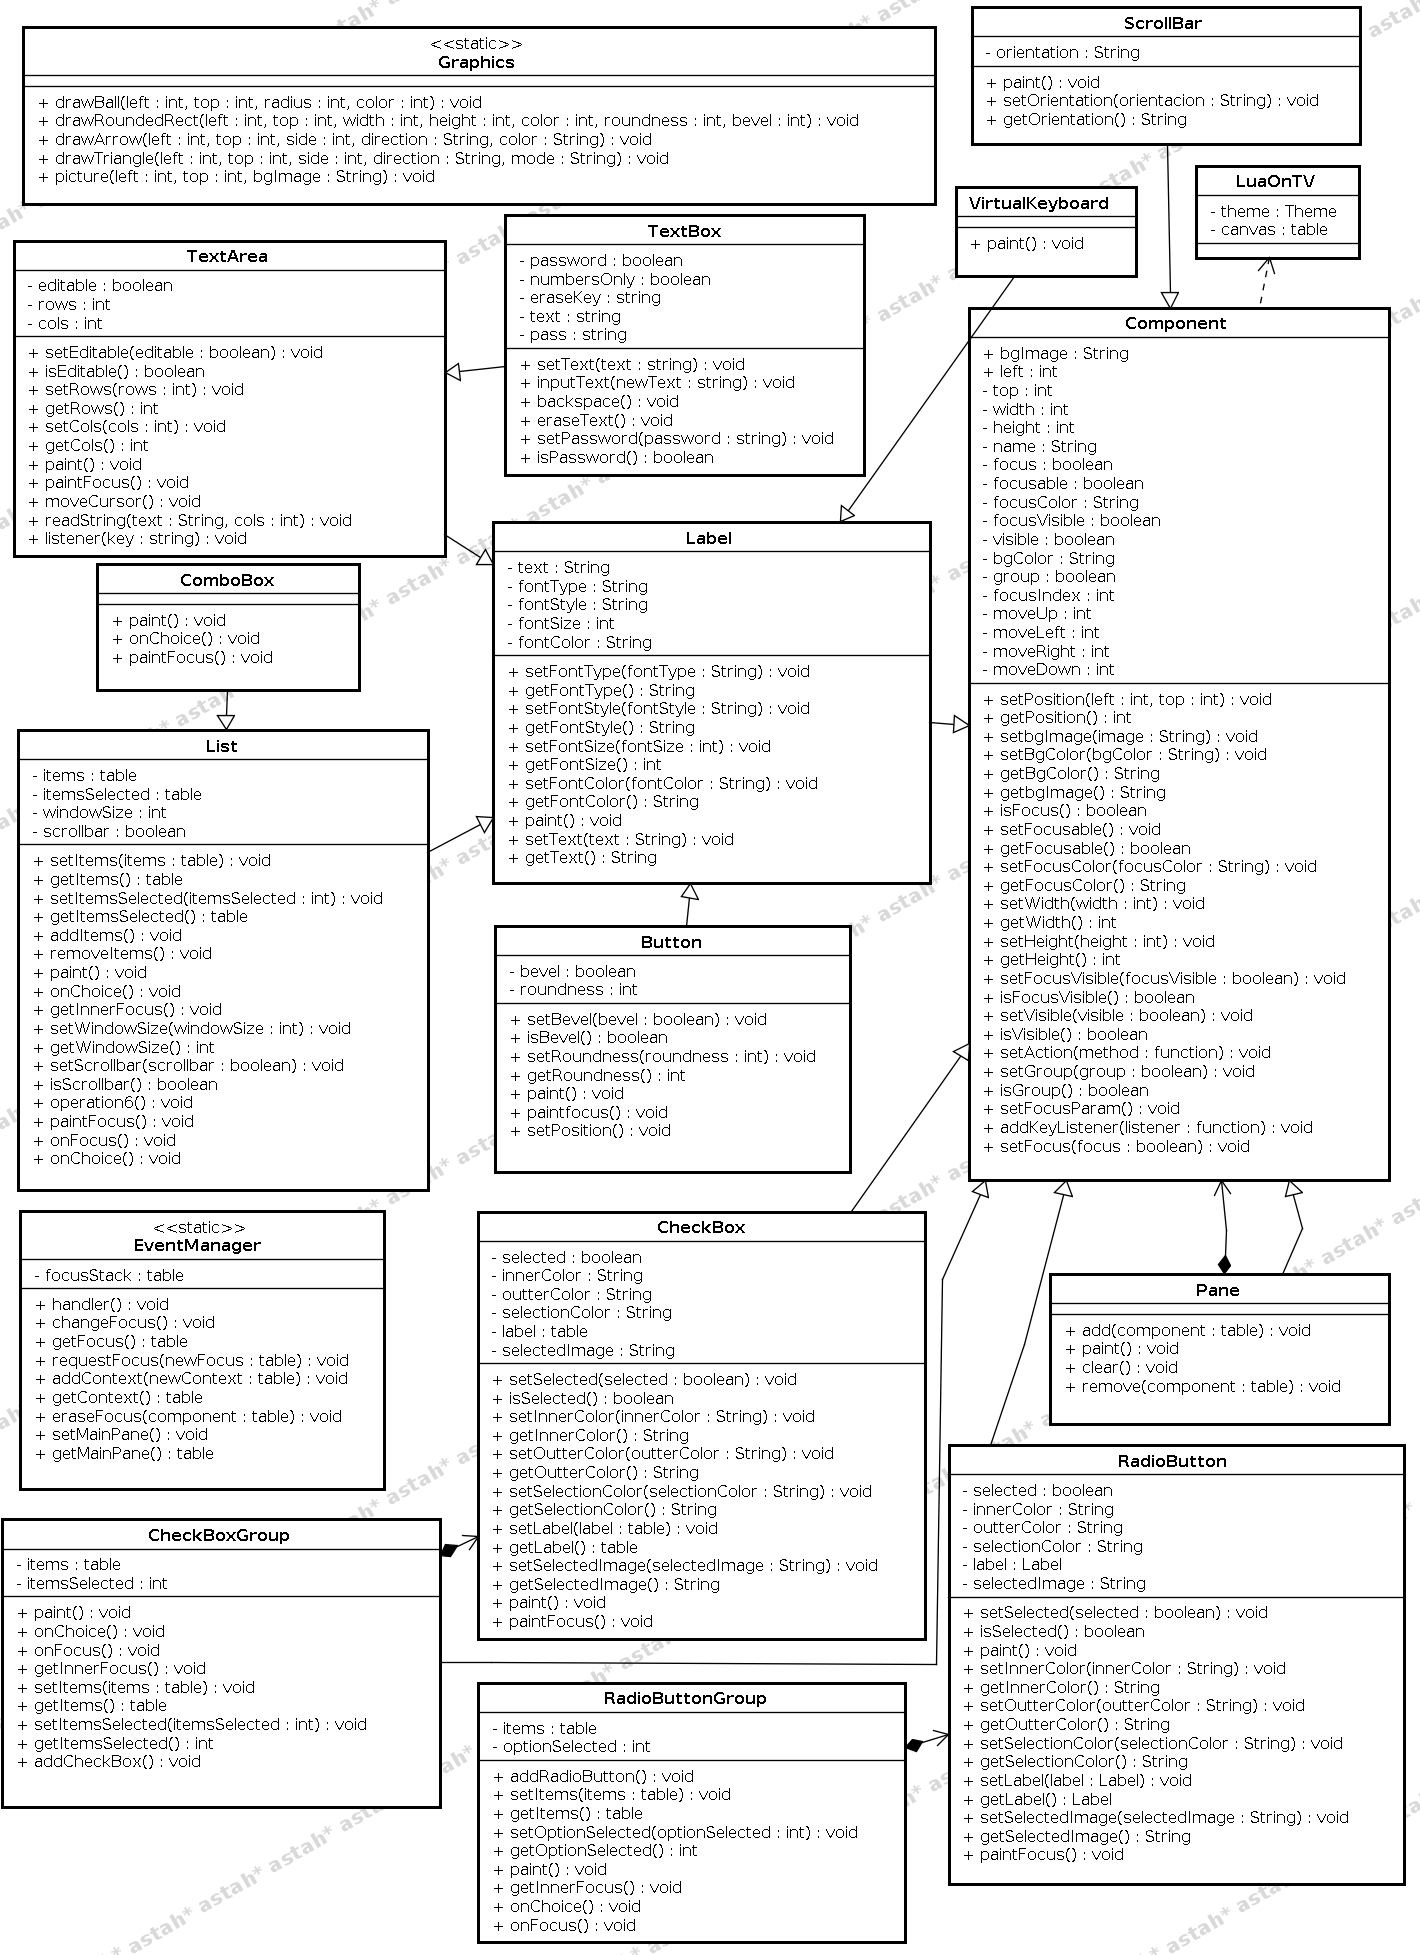
\includegraphics[width=1.12\textwidth]{LuaOnTV-Components.png}
	\captionof{figure}{Novo diagrama de classes do LuaOnTV}
	\label{fig:luaontv-classdiagram}
\end{center}

Neste diagrama, a classe \textit{EventManager} tem um papel fundamental no \textit{framework}, pois ela é responsável pelo tratamento
dos eventos ocorridos na aplicação, principalmente os eventos de pressionamento de teclas,
controlando a entrada de dados na tela e a navegação entre os campos por meio das teclas direcionais
do controle remoto. Desta forma, a Figura \ref{fig:event-manager-statemachine}
apresenta um gráfico de máquinas estados desta classe.

\begin{center}
	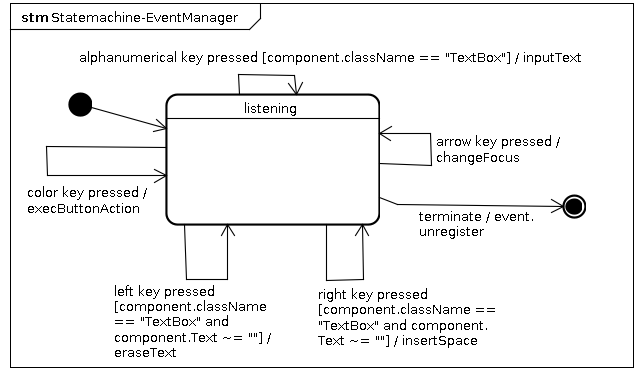
\includegraphics[width=0.8\textwidth]{LuaOnTV-Statemachine-EventManager.png}
	\captionof{figure}{Gráfico de Máquinas de Estados da classe \textit{EventManager}}
	\label{fig:event-manager-statemachine}
\end{center}

Um dos principais novos recursos implementados no LuaOnTV 
foi o suporte a temas. A Figura \ref{fig:luaontv-themes} apresenta as classes relacionadas a tal recurso.

\begin{center}
	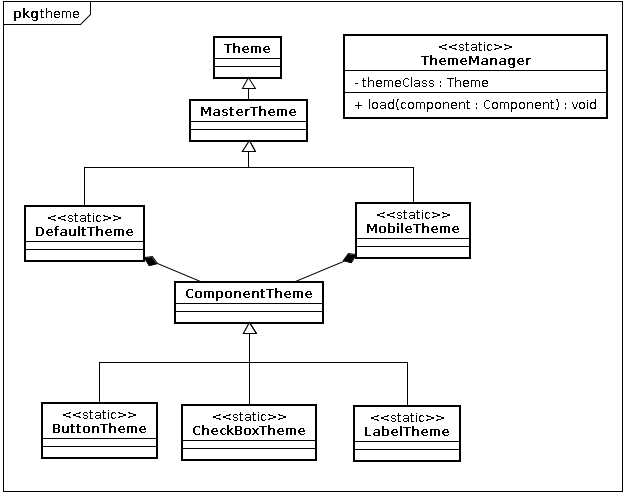
\includegraphics[width=0.8\textwidth]{LuaOnTV-Themes.png}
	\captionof{figure}{Classes relacionadas ao novo recurso de temas do LuaOnTV}
	\label{fig:luaontv-themes}
\end{center}

Como mencionado anteriormente, o LuaOnTV utiliza os módulos \textit{canvas} e \textit{event} do Ginga-NCL.
Assim, a Figura \ref{fig:luaontv-component-diagram} apresenta um diagrama de componentes,
mostrando como os elementos do LuaOnTV e do Ginga-NCL se relacionam.
O LuaOnTV possui dois pacotes principais: \textit{Components}, contendo as classes
que implementam os componentes visuais e não visuais; e \textit{Themes}, contendo
as classes que implementam os temas. O LuaOnTV cria uma camada
de abstração para os módulos \textit{canvas} e \textit{event} do Ginga-NCL, provendo
funcionalidades de mais alto nível.

\begin{center}
	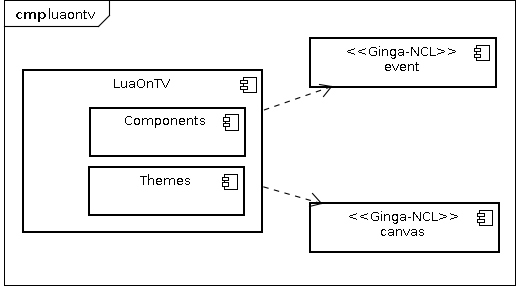
\includegraphics[width=0.7\textwidth]{LuaOnTV-Component-Diagram.png}
	\captionof{figure}{Diagrama de Componentes do LuaOnTV}
  \label{fig:luaontv-component-diagram}
\end{center}



\chapter{Framework de comunicação de dados} \label{cap:ncluasoap}

A arquitetura apresentada no Capítulo \ref{cap:arquitetura-tcommerce}
utiliza protocolos de comunicação HTTP e SOAP. Tais protocolos foram
implementados em um \textit{framework} de comunicação a ser apresentado neste capítulo.

\section{Integração entre \textit{Web} e TV}
%----------------DEFINE FORMA CORRETA DE HIFENIZAÇÃO PARA ALGUMAS PALAVRAS ----------------
\hyphenation{res-pos-ta}
\hyphenation{res-pos-tas}
\hyphenation{exis-tem}
\hyphenation{va-lor}
\hyphenation{va-lo-res}
\hyphenation{im-pe-ra-ti-va}
\hyphenation{im-pe-ra-ti-vas}
\hyphenation{im-pe-ra-ti-vo}
\hyphenation{im-pe-ra-ti-vos}
\hyphenation{ou-tra}
\hyphenation{ou-tro}
\hyphenation{ou-tras}
\hyphenation{ou-tros}
\hyphenation{pro-ble-ma}
\hyphenation{res-tri-to}
\hyphenation{res-tri-tos}
\hyphenation{res-tri-ta}
\hyphenation{res-tri-tas}
\hyphenation{me-lho-rar}
\hyphenation{fun-cio-na-li-da-de}
\hyphenation{fun-cio-na-li-da-des}
\hyphenation{apre-sen-ta-do}
\hyphenation{mo-de-lo}
\hyphenation{apre-sen-ta-dos}
\hyphenation{apre-sen-ta-da}
\hyphenation{apre-sen-ta-das}
\hyphenation{do-cu-men-to}
\hyphenation{LuaSQL}
\hyphenation{e-co-no-mi-zar}
%\hyphenation{ca-rac-te-rís-ti-ca}
%\hyphenation{ca-rac-te-rís-ti-cas}
%----------------DEFINE FORMA CORRETA DE HIFENIZAÇÃO PARA ALGUMAS PALAVRAS ----------------

Um dos grandes atrativos da TV Digital (TVD) é com certeza a interatividade. Existem diversas categorias
de aplicações interativas como jogos, informações (notícias, horóscopo, previsão do tempo, etc), 
educação (\textit{T-Learning}), governo eletrônico (\textit{T-Government}), comércio eletrônico (\textit{T-Commerce}), 
saúde (\textit{T-Health}), bancárias (\textit{T-Banking}) e outras, como apresentado em \cite{fernandez2008aplicaciones},
\cite{de-usabilidade} e \cite{tgov2010barbosa}.

O nível de interatividade das aplicações vai desde a chamada interatividade local
(onde os usuários/telespectadores podem acessar apenas os dados enviados pela emissora, por radiodifusão)
até a interatividade plena (onde os usuários/telespectadores dispõem de um canal de retorno, permitindo
enviar e receber dados em uma rede como a \textit{Internet}) \cite{soares2009programando}. 

Tais aplicações que permitem interatividade plena precisam utilizar protocolos de comunicação 
padrões e consolidados na \textit{Internet} (como TCP, HTTP e SOAP) para garantir a interoperabilidade
com outros sistemas. 

Utilizando os protocolos citados, é possível garantir a convergência entre \textit{Web} e TV.
Com isto, as aplicações de TVDi podem ser enriquecidas com conteúdo proveniente da \textit{Internet},
como é o caso da aplicação que busca conteúdo na Wikipédia, baseada nas \textit{tags}
do programa em exibição, obtidos a partir do Guia Eletrônico de Programação 
(cujas informações são enviadas pela emissora), 
como apresentado em \cite{socialnets-tvd2010ghisi}.

A norma do sub-sistema Ginga-NCL do \textit{middleware} Ginga define 
apenas a obrigatoriedade do protocolo TCP. Quaisquer protocolos acima da camada de transporte
precisam ser implementados pelo desenvolvedor de aplicações. 

%\subsection{Objetivos}
Tendo em vista o cenário supracitado, são apresentados neste trabalho os projetos NCLua HTTP e NCLua SOAP: implementações dos protocolos HTTP e SOAP, respectivamente, para o sub-sistema Ginga-NCL, utilizando linguagem Lua, que permitem a convergência
entre aplicações de TVDi e a \textit{Web}.

%\subsection{Motivação}
A escolha de implementação de HTTP e SOAP partiu da inexistência de versões livres e de código aberto de tais protocolos para o Ginga-NCL.
Até onde sabe-se, o NCLua HTTP e NCLua SOAP são as primeiras implementações livremente disponibilizadas.

%Incluir isto apenas no artigo, pois não faz sentido na dissertação
\begin{comment}
O artigo está organizado como segue. 
Na Seção \ref{sec:problema} é apresentado o problema de consumo de \textit{Web Services} em aplicações
de TVDi no Ginga-NCL. 
Na Seção \ref{sec:trabs-rel} são apresentadas as tecnologias e trabalhos relacionados.
Na Seção \ref{sec:modulos-implementados} é apresentada a proposta implementada para prover o consumo de \textit{Web Services} em aplicações de TVDi. 
Na Seção \ref{sec:resultados} são apresentados os resultados alcançados e exemplos de utilização dos módulos desenvolvidos.
Na Seção \ref{sec:conclusao} são tecidas as conclusões. Por fim, na Seção \ref{sec:trabalhos-futuros} são esboçados os trabalhos futuros.
\end{comment}

\section{Delimitação do Problema} \label{sec:problema}

Apesar de Lua ser uma linguagem extensível \cite{ierusalimschy2007evolution}, principalmente pela capacidade de utilizar módulos construídos em linguagem C, e de existirem vários destes módulos para as mais diversas finalidades, tais módulos binários não podem ser utilizados em aplicações interativas de TV Digital enviadas via \textit{broadcast}, devido a questões de segurança, uma vez que um módulo escrito em linguagem C pode ter acesso a qualquer funcionalidade do sistema operacional (embarcado juntamente com o \textit{middleware} no receptor de TV Digital). 

Em \cite{braga-introducao} são citadas algumas ameaças de segurança em sistemas de TVDi, como 
transação fraudulenta (perda/roubo de dados), pirataria de conteúdo,  falsificação, violação ou corrupção das aplicações 
e uso ilegítimo de serviços do provedor.

Tais ameaças podem ser potencializadas com o uso de módulos binários. Além do mais, a compilação de módulos em C gera código nativo dependente de plataforma, o que não garante que a aplicação executará em qualquer receptor \cite{costa-seguranca}.
Somente aplicações residentes podem ser desenvolvidas em linguagens compiladas como C.

Com isto, para haver, em aplicações NCLua de TVDi, algumas das funcionalidades dos módulos binários citados, é preciso
implementar módulos inteiramente em linguagem Lua, cujo ciclo de vida é controlado pelo \textit{middleware} Ginga\cite{abnt200815606}.

\section{Tecnologias Envolvidas e Trabalhos Relacionados} \label{sec:trabs-rel}

Nesta seção são apresentadas as tecnologias envolvidas no desenvolvimento da solução
apresentada e os trabalhos relacionados.

\subsection{Tecnologias de \textit{Web Services}} \label{sec:ws}

SOAP é um protocolo padrão da \textit{World Wide Web Consortium} (W3C) que permite a aplicações oferecerem seus serviços na \textit{Internet}, em uma arquitetura distribuída no modelo cliente/servidor. O protocolo permite troca de mensagens e chamadas de procedimentos remotos. 
Tais serviços podem ser providos e consumidos por aplicações desenvolvidas em diferentes linguagens e plataformas. 
Isto permite a interoperabilidade entre diferentes aplicações, por meio da troca de documentos XML, 
usando algum protocolo de transporte como o HTTP \cite{soap-spec} \cite{curbera2002unraveling} \cite{newcomer2002understanding}.

Um dos grandes benefícios do protocolo SOAP para a integração de aplicações é a 
sua linguagem para descrição dos serviços disponibilizados, a \textit{Web Service Description Language} (WSDL).
De forma padronizada, manual ou automatizadamente, uma aplicação cliente pode conhecer os serviços
disponibilizados por um \textit{Web Service} lendo o documento WSDL do serviço (também em formato XML)\cite{soap-spec}.

Os \textit{Web Services} permitem a construção de aplicações distribuídas pela \textit{Internet}, garantindo a centralização
de regras de negócios em servidores de aplicações, encarregados de toda a carga de processamento
de tais regras. Considerando-se isto, \textit{Web Services} são ideais para aplicações clientes executando em
sistemas com restritos recursos de \textit{hardware}, como celulares e \textit{Set-top Boxes}, estes últimos
sendo o foco do presente trabalho. Além de desonerar os clientes da carga de processamento, alterações nas regras
de negócio não requerem a atualização das aplicações clientes.

\begin{comment}
\subsection{O protocolo HTTP}

O \textit{Hyper Text Transfer Protocol} (HTTP) é um protocolo de comunicação (da camada de aplicação do modelo OSI) 
utilizado para a transferência de hipertexto pela Web. 
Ele é uma especificação da W3C e da \textit{Internet Engeneering Task Force} (IETF), cuja versão mais recente, o HTTP 1.1,
é definido pela RFC 2616 \cite{rfc2616}.

O HTTP é um dos protocolos mais populares na Web, utilizado pela grande maioria dos serviços hospedados na núvem.
Ele é um protocolo baseado no modelo cliente/servidor de requisição/resposta. 
Por padrão ele trafega dados utilizando a porta 80 
(normalmente liberada para navegação na Web), sendo, desta forma, amigável a \textit{firewalls}. 
Com isto, o protocolo permite a comunicação entre
aplicações por meio da Intenet. Desta forma, o HTTP é o principal protocolo de transporte utilizado
por aplicações SOAP. Ele define um formato simples e padronizado para a tranferência de documentos como HTML e XML,
este último, utilizado nas trocas de mensagens do protocolo SOAP.

O protocolo há bastante tempo é uma tecnologia universalizada na Web, e sua simplicidade 
e concisão garantem que ele não aumente a latência da transmissão e nem o processamento das mensagens
enviadas e recebidas. Desta forma, ele pode ser utilizado sem problemas 
em redes com banda estreita e dispositivos com recursos de hardware restritos.

A sua natureza independente de linguagem e plataforma, permite que hajam diversas implementações 
do protocolo. Na parte servidora do mesmo, sua implementação é integrada em softwares conhecidos
como servidores \textit{Web}/HTTP.

Desde a versão 1.0 do mesmo, ele permite não somente o tráfego de hipertexto como também
de qualquer formato de arquivo definido pelos tipos MIME (\textit{Multipurpose Internet Mail Extensions}), 
cuja especificação é dada pela RFC 2045 \cite{rfc2045}.

Até o HTTP/1.0, o protocolo não permitia conexões persistentes, sendo um protocolo \textit{stateless},
não guardando qualquer informações no servidor sobre as requisições recebidas, o que 
requer menos uso de memória por parte do servidor, ajudando a reduzir a sobrecarga do mesmo.
Desta forma, para o servidor, cada requisição é uma nova requisição.
A versão 1.1 introduziu o uso de conexões persistentes, no entanto, a forma tradicional ainda
é a mais utilizada, principalmente no transporte de conteúdo HTML (páginas Web) e XML.
\end{comment}

\subsection{Lua e os \textit{scripts} NCLua} \label{sec:lua-nclua}

Lua é a linguagem imperativa utilizada pelo sub-sistema Ginga-NCL para o desenvolvimento
de aplicações procedurais. Ela tem como grandes vantagens sua simplicidade, eficiência e portabilidade. 
Tais características são extremamente importantes em uma linguagem a ser utilizada em dispositivos com recursos de hardware restritos, 
como os conversores de TV Digital (\textit{Set-top Boxes}). Além de tudo, Lua é livre de \textit{royalties}, o que permite
que a mesma seja embarcada em \textit{Set-top Boxes} sem onerar o custo dos equipamentos. Este é um requisito
muito importante, considerando as características sócio-econômicas do Brasil, a intenção do governo de 
utilização da TV como meio para inclusão digital e sua presença na grande maioria
dos lares brasileiros.

Como a linguagem NCL é apenas declarativa, a inclusão de características imperativas
a uma aplicação de TVDi para o Ginga-NCL é possibilitada por meio dos chamados
NCLua, \textit{scripts} Lua funcionando como nós de mídia dentro de um documento NCL 
\cite{abnt200815606} \cite{soares2007ginga}. 

Tais \textit{scripts} aumentam o poder das aplicações de TVDi, possibilitando a construção
de aplicações sofisticadas, seguindo paradigmas como Programação Estruturada e Programação Orientada a Objetos,
com definição de regras de negócio na aplicação, interoperabilidade com sistemas na \textit{Internet}
por meio de protocolos como HTTP e SOAP, entre outros recursos.

O que diferencia os \textit{scripts} NCLua de \textit{scripts} Lua convencionais é a possibilidade de comunicação
bidirecional entre este e o documento NCL. Tal comunicação acontece por meio de eventos, como definido
na norma do Ginga-NCL em \cite{abnt200815606}. Segundo \cite{sant2008nclua} 
"essa integração deve seguir critérios que não afetem os princípios da linguagem declarativa, mantendo uma separação bem definida 
entre os dois ambientes". Para isto, nenhuma alteração nas linguagens NCL ou Lua foi necessária, o que garante a evolução
independente das linguagens, como ressalta \cite{sant2008nclua}. 

A integração entre as linguagens NCL e Lua foi feita para ser minimamente intrusiva,
garantindo uma separação entre a forma declarativa e a procedural de desenvolver uma aplicação para o Ginga-NCL.
Assim, o código NCLua deve ser escrito obrigatoriamente em um arquivo separado do NCL. 
Isto permite uma clara divisão de tarefas entre profissionais da área de \textit{design} e da área de programação \cite{sant2008nclua}.
A integração entre outras linguagens como HTML e \textit{JavaScript} é bastante intrusiva, onde, muitas vezes, código \textit{JavaScript} é intercalado
com código HTML.

O tratamento de eventos e as particularidades associadas a aplicações de TVDi, desenvolvidas em linguagem Lua, 
são implementadas por módulos adicionais à Linguagem, definidos na norma do Ginga-NCL \cite{abnt200815606}.
Isto permite que a linguagem se mantenha inalterada para o contexto de TV Digital. 
Os módulos disponíveis em NCLua, utilizados neste trabalho são: \textbf{\textit{event}}, 
que permite a comunicação bidirecional entre um NCL e um NCLua;
e \textbf{\textit{canvas}}, que disponibiliza uma API para desenhar imagens e primitivas gráficas.

\subsection{Protocolo TCP no Ginga-NCL} \label{sec:tcp}

A norma do Ginga-NCL \cite{abnt200815606} define a disponibilidade do protocolo TCP para ser utilizado pelas aplicações interativas.
Como os objetos NCLua têm a característica de poderem ser orientados a eventos, o módulo \textit{event} permite a captura e tratamento de eventos, possibilitando a comunicação assíncrona entre o formatador NCL e um objeto NCLua.

A implementação do protocolo TCP deve ser disponibilizada por meio do módulo \textit{event}. A norma especifica uma classe de eventos 
denominada \textit{tcp}. Assim, por meio das funções do módulo \textit{event}, um objeto NCLua pode enviar 
requisições e receber respostas usando o protocolo TCP.

Devido à característica assíncrona do módulo \textit{event}, o tratamento de requisições TCP em NCLua não é trivial. 
Para facilitar o uso de tal protocolo, pode-se recorrer ao recurso de co-rotinas da linguagem Lua. 
Segundo \cite{ierusalimschy2006programming}, uma co-rotina é similar a um \textit{thread} (no sentido de \textit{multithreading}).
No entanto, co-rotinas são colaborativas, sendo executada apenas uma por vez.

A documentação de NCLua disponível em \cite{doc-nclua}, apresenta um módulo que utiliza co-rotinas para facilitar 
o tratamento das requisições assíncronas da classe de eventos \textit{tcp}. No entanto, mesmo tal módulo ainda não
permite encapsular todos os detalhes do envio da requisição em apenas uma função, para simplificar 
o uso para os desenvolvedores de aplicações interativas.

A Figura \ref{fig:tcp-state-machine} apresenta um gráfico de máquinas de estados
da realização de uma conexão TCP no Ginga-NCL, utilizando o módulo \textit{tcp.lua}.
Em um processo convencional, a aplicação estabelece uma conexão
a um servidor. Após estabelecida a conexão ela envia uma requisição
e fica aguardando o retorno. A função \textit{tcp.receive} é executada até
que não haja mais dados a serem recebidos, realizando
a desconexão.

\begin{center}
	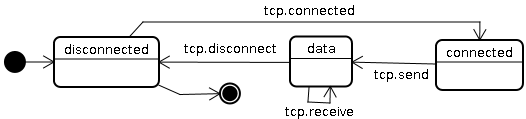
\includegraphics[scale=0.5]{ncluasoap-Statemachine-TCP.png}
	\captionof{figure}{Diagrama de Máquinas de Estados do Módulo \textit{tcp.lua}}
	\label{fig:tcp-state-machine}
\end{center}

A Figura \ref{fig:tcp-state-machine-coroutines} apresenta um gráfico de máquinas de estados
do mesmo módulo, porém, do ponto de vista das co-rotinas em execução (que são semelhantes
a \textit{threads}, como já discutido anteriormente). O processo de uso do módulo
é iniciado internamente com a criação de uma corotina (que é criada suspensa,
não automaticamente iniciando sua execução). A função \textit{coroutine.resume}
inicia a execução da co-rotina. Quando é solicitada uma tentativa de
conexão, a co-rotina é suspensa, ficando aguardando até que 
a conexão seja estabelecida, ocorrendo tudo de forma assíncrona.
Neste momento, a co-rotina é novamente resumida (continuando a execução),
permitindo que seja enviada uma requisição ao servidor (\textit{tcp.send}).
Tal função retorna imediatamente. Para a obtenção da resposta
da requisição (que também será feita de forma assíncrona), 
é preciso usar a função \textit{tcp.receive}, que faz com que a co-rotina
seja suspensa novamente, até que algum dado da resposta seja obtido.
A função \textit{tcp.receive} pode ser chamada iterativamente até que
não haja mais nenhum dado a ser retornado para a aplicação.

Todo este processo apresentado nos gráficos de máquinas de estado,
mesmo utilizando as facilidades providas pelo módulo \textit{tcp.lua},
não são encapsulados para facilitar o uso. O módulo citado
apenas facilita o gerenciamento das chamadas assíncronas.
A implementação do NCLua HTTP e NCLua SOAP encapsulam todas
essas chamadas de funções, tornando o processo bem mais simples para
o desenvolvedor, disponibilizando uma simples função
para realização de uma requisição.

É importante lembrar que tal abordagem é útil em cenários
de aplicações \textit{stateless}, que não mantém
estado entre uma requisição e outra, como o caso do HTTP/1.0
e das chamadas SOAP. Aplicações que precisem manter a conexão
aberta, como mensageiros instantâneos, precisam utilizar
diretamente as funções do módulo tcp.lua.

\begin{center}
	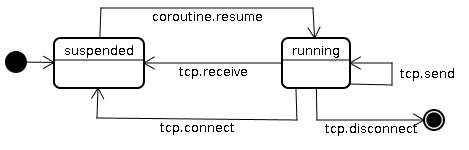
\includegraphics[scale=0.5]{ncluasoap-Statemachine-TCP-Coroutines.png}
	\captionof{figure}{Diagrama de Máquinas de Estados do Módulo \textit{tcp.lua} (co-rotinas em execução)}
	\label{fig:tcp-state-machine-coroutines}
\end{center}

\subsection{Implementações de SOAP}

Existem diversos \textit{toolkits} para provimento e consumo de \textit{Web Services}, disponíveis em diferentes linguagens e plataformas.
Nas sub-seções seguintes são apresentados alguns destes.

\subsubsection{LuaSOAP}

Para acesso a \textit{Web Services} SOAP a partir de aplicações Lua, pode-se utilizar o módulo LuaSOAP \cite{luasoap}.

O protocolo SOAP envolve a troca de mensagens em formato XML, permitindo a interoperabilidade entre sistemas desenvolvidos
em diferentes linguagens. No entanto, para fazer o \textit{parse} de arquivos XML, o LuaSOAP depende da biblioteca
\textit{Expat} \cite{expat}\cite{cooper1999using}, que é um \textit{parser} XML desenvolvido em linguagem C, cujos problemas de uso
em aplicações de TVDi foram apresentados na Seção \ref{sec:problema}. O projeto também depende da biblioteca \textit{LuaSocket},
que também usa módulos em C.

O LuaSOAP não permite a geração automática de \textit{stubs} para realizar a chamada aos métodos remotos do \textit{Web Service}.
Desta forma, o desenvolvedor precisa ler o documento WSDL e obter as informações sobre o método que deseja invocar.
A última atualização do projeto foi em 2004, o que mostra que o mesmo não está acompanhando as novas
versões de Lua, como a 5.1 utilizada na implementação de referência do Ginga.

Uma das vantagens do projeto é que as chamadas aos métodos remotos no \textit{Web Service} são síncronas, o que facilita
bastante o uso.

\subsubsection{gSOAP}

O gSOAP é classificado como um \textit{Software Development Kit} (SDK) para permitir que aplicações legadas, sistemas embarcados e de tempo real, desenvolvidos em linguagens C, C++ e Fortran, possam consumir \textit{Web Services} \cite{van2005gsoap}. O projeto possui um utilitário capaz de gerar \textit{stubs} em C/C++, a partir do documento WSDL do serviço. Em tal \textit{stub} são incluídos métodos \textit{proxies} para realizar chamadas aos métodos remotos do serviço, tornando-as transparentes para a aplicação cliente.

As chamadas realizadas com gSOAP também são síncronas, o que facilita muito o desenvolvimento das aplicações clientes,
pois o envio da requisição e tratamento da resposta pode ser todo feito em uma única rotina.

Pelo fato do projeto ser desenvolvido em C, o mesmo só poderia ser utilizado
em aplicações de TVD residentes no conversor digital, como já comentado na Seção \ref{sec:problema}.
A utilização de linguagens compiladas como C/C++ permite que o \textit{(un)marshalling} 
seja feito em tempo de compilação, o que garante que a aplicação terá maior velocidade 
na execução. No entanto, a necessidade de tal processo de compilação elimina
a grande vantagem do dinamismo existente em linguagens interpretadas como Lua.

\subsubsection{Apache Axis}

Em \cite{davis2005latency} são apresentados alguns outros \textit{toolkits} para provimento e consumo de \textit{Web Services}. Um dos projetos citados é o Apache Axis, uma implementação de SOAP para Java e C, que tem, como uma das vantagens, o uso do \textit{parser} XML SAX, o qual é completo e bastante eficiente. Ele também possui a vantagem de gerar \textit{stubs} Java ou C, a partir do documento WSDL.

Mesmo o Ginga permitindo o uso de Java, o Apache Axis pode não ser uma solução ideal para
aplicações de TVD, uma vez que inclui o SAX como \textit{parser} XML.
Considerando a capacidade de hardware restrita dos conversores de TV Digital, tal \textit{parser} pode não ser ideal 
em tais equipamentos, além de poder não estar em conformidade com as normas do 
Sistema Brasileiro de TV Digital (SBTVD). \textit{Parsers} mais simples como o NanoXML\footnote{\url{http://nanoxml.sourceforge.net}}, 
que demandam menos capacidade de processamento, podem ser mais adequados neste cenário.
Por fim, o Apache Axis não atende a um dos requisitos elicitados: ser implementado em Lua para uso direto por aplicações NCLua.

\begin{comment}
\begin{center}
	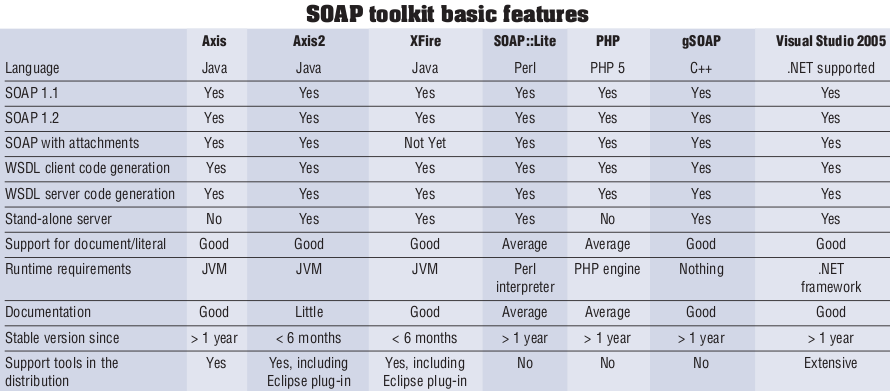
\includegraphics[scale=0.4]{soap-toolkits.png}
	\captionof{figure}{Tabela comparativa entre \textit{toolkits} SOAP \cite{louridas2006soap}}
	\label{fig:tabela-comparativa}
\end{center}
\end{comment}

%------------------------------------------------------------------------------------------------------------------------
\section{Proposta de Novas Implementações de HTTP e SOAP} \label{sec:modulos-implementados}

O Ginga-NCL provê protocolos de rede até o TCP, assim, qualquer protocolo acima da camada de transporte do modelo OSI precisa ser implementado.
Como o envio de envelopes SOAP é normalmente feito por HTTP, tal protocolo precisou ser implementado como um módulo NCLua,
ao qual denominou-se NCLua HTTP, que será utilizado pelo NCLua SOAP.

\subsection{Decisões de Projeto}

Para o desenvolvimento do projeto, optou-se por seguir o padrão
de módulos, amplamente utilizado na atual versão da linguagem Lua.
Um módulo encapsula funções com objetivos correlatos
e tal padrão é bastante conhecido dos programadores Lua.

Tal modelo segue o paradigma de programação estruturada, assim,
um módulo consiste de um conjunto de funções que são chamadas
pelo desenvolvedor que for utilizá-lo.

Na geração das requisições SOAP, optou-se por fazer o \textit{(un)marshalling}
de XML para tabelas Lua por estas serem as estruturas de dados
padrões disponibilizadas pela linguagem e por serem estruturas
bastante flexíveis e fáceis de manipular, devendo ser de conhecimento
de qualquer programador Lua.

Como o conteúdo das requisições HTTP e SOAP é apenas texto, formatado
segundo o padrão de cada protocolo, a geração e formatação
deste conteúdo foi bastante simples e direta. Devido a
\textit{strings} em Lua serem imutáveis\cite{ierusalimschy2006programming},
para economizar memória na concatenação das \textit{strings} que compõe
cada requisição, as tabelas de Lua foram utilizadas
como um \textit{buffer} de \textit{strings} para otimizar o uso de memória RAM.

Na obtenção dos resultados, procurou-se facilitar ao máximo
tal tarefa para o desenvolvedor, permitindo que ele
tenha acesso direto aos dados retornados, sem precisar
conhecer o caminho dentro do XML de retorno onde
a resposta está armazenada, assim como fazem outros \textit{toolkits} SOAP
como a API JAX-WS.

Quanto ao \textit{parser} XML escolhido, não haviam muitas opções
implementadas inteiramente em Lua. 
Todas as implementações testadas foram encontradas
em \url{http://lua-users.org} e em \cite{ierusalimschy2006programming}.
Optou-se pelo uso do LuaXML\footnote{\url{http://lua-users.org/wiki/LuaXml}},
pois foi a implementação que fazia o \textit{unmarshalling} de XML
para tabelas Lua com a estrutura mais simples e fácil de manipular.
Além do mais, as outras implementações encontradas não funcionaram
adequadamente para XML's mais complexos retornados
por alguns \textit{Web Services}.

\subsection{NCLua HTTP} \label{sec:ncluahttp}

O NCLua HTTP\footnote{\url{http://ncluahttp.manoelcampos.com} e \url{http://labtvdi.unb.br}} implementa alguns dos principais recursos do protocolo HTTP/1.0. 
Ele é um módulo escrito inteiramente em linguagem Lua
para ser utilizado em \textit{scripts} NCLua. O mesmo utiliza o protocolo TCP da forma como especificado na norma do Ginga-NCL
em \cite{abnt200815606}, por meio da classe de eventos \textit{tcp} de NCLua.
Pela simplicidade do protocolo HTTP, o módulo possui apenas algumas funções que permitem a geração
de requisições e tratamento de respostas. Atualmente existem os seguintes recursos implementados:

\begin{itemize}
  \item suporte à autenticação básica, uso de portas específicas e download de arquivos;
  \item suporte à requisições \textit{GET} e \textit{POST};
  \item passagem de parâmetros em requisições \textit{POST};
  \item suporte à passagem de cabeçalhos HTTP e definição de \textit{User-Agent};
  \item suporte à separação automática dos dados do cabeçalho e do corpo da resposta de uma requisição.
\end{itemize}

\subsection{NCLua SOAP} \label{sec:ncluasoap}
O NCLua SOAP\footnote{\url{http://ncluasoap.manoelcampos.com} e \url{http://labtvdi.unb.br}} implementa as principais funcionalidades do protocolo SOAP 1.1 e 1.2. 
Ele também é um módulo inteiramente
escrito em Lua, que faz o \textit{parse} de arquivos XML, 
realizando o \textit{marshalling} e \textit{unmarshalling} de/para tabelas Lua, permitindo que o desenvolvedor Lua
trabalhe com a estrutura de dados principal da linguagem: o tipo \textit{table}.

O módulo utiliza o NCLua HTTP para transportar as mensagens SOAP. Assim, todos os detalhes do protocolo HTTP são 
encapsulados pelo respectivo módulo. Com isto, a implementação do SOAP fica bastante simplificada, tornando o código
fácil de ser mantido. O NCLua SOAP encarrega-se apenas de gerar o XML da requisição SOAP, utilizando
o NCLua HTTP para enviar tal XML no corpo da mensagem. O \textit{parse} e \textit{unmarshalling} do XML para uma tabela Lua
é todo encapsulado pelo módulo LuaXML\footnote{\textit{Parser} XML escrito inteiramente em Lua, adaptado para funcionar com Lua 5}. 

Um importante recurso, não disponível em implementações como o LuaSOAP (citada na Seção \ref{sec:trabs-rel}),
e que facilita bastante a utilização do módulo, é a simplificação 
do XML retornando como resposta, que é convertido (\textit{unmarshalling}) automaticamente para uma tabela Lua.
Para demonstrar este recurso, utilizar-se-á o \textit{Web Service} de consulta de endereço a partir de um CEP,
disponível em \url{http://www.bronzebusiness.com.br/webservices/wscep.asmx}. Tal WS possui um método chamado "cep",
que recebe um determinado CEP e retorna o endereço referente ao mesmo.
O XML do retorno do método "cep", convertido para uma tabela Lua, é semelhante ao mostrado na Listagem \ref{list:cepws}.

A estrutura da tabela reflete o código XML retornado. Como pode ser visto, o elemento
da tabela que contém de fato os dados do endereço retornado (tbCEP) está envolvido em 
várias outras tabelas que não contém dado algum, sendo estruturas completamente
desnecessárias para a aplicação NCLua. Com isto, para o desenvolvedor
poder acessar, por exemplo, a cidade do CEP indicado, precisará 
conhecer toda a estrutura retornada, utilizando uma instrução como
\textit{result.cepResult.diffgr.NewDataSet.tbCEP.cidade}.

Para esconder estes detalhes do desenvolvedor, o NCLua SOAP simplifica qualquer
resultado que contenha estruturas desnecessárias, como o mostrado na Listagem \ref{list:cepws}.

\begin{lstlisting}[caption=Exemplo de tabela Lua gerada a partir do XML de uma resposta SOAP, label=list:cepws, language=lua]
{ cepResult =  {  diffgr = { NewDataSet = {  tbCEP = {
   nome="Cln 407", bairro="Asa Norte", UF="DF", cidade="Brasilia"
} } } } }
\end{lstlisting}

Desta forma, para o exemplo citado, a tabela Lua (gerada a partir do XML de retorno da requisição) 
ficará como apresentado na Listagem \ref{list:ncluasoap-tb}, o que simplifica
o acesso aos elementos da estrutura retornada, permitindo, por exemplo, que o campo
cidade seja acessado utilizando-se apenas a instrução \textit{result.cidade}.

\begin{lstlisting}[caption=Exemplo de simplificação de retorno de resposta SOAP pelo NCLua SOAP, label=list:ncluasoap-tb, language=lua]
{   nome="Cln 407", bairro="Asa Norte", UF="DF", cidade="Brasilia"   }
\end{lstlisting}

O módulo ainda conta com um \textit{script} (\textit{wsdlparser.lua}), em fase inicial de implementação, que realiza
o \textit{parse} de um documento WSDL e obtém algumas das informações que precisa-se
passar ao NCLua SOAP para que ele realize a requisição 
(como o \textit{namespace} do serviço, o nome do método desejado e a lista de parâmetros de entrada).
Atualmente o \textit{script} apenas lê o WSDL e exibe algumas
das informações citadas, cabendo ao desenvolvedor copiá-las e passá-las ao método \textit{call} do
NCLua SOAP para realizar a chamada a um determinado método remoto. No entanto, 
a extração de tais informações já ajuda de alguma forma, principalmente
os usuários menos experientes na tecnologia de \textit{Web Services} e no NCLua SOAP.

Para resumir, as características principais do NCLua SOAP são:

\begin{itemize}
  \item suporte a SOAP 1.1 e 1.2;
  \item suporte a parâmetros de entrada e saída do tipo \textit{struct} e \textit{array}
   (sendo feito \textit{marshalling} e \textit{unmarshalling} de/para tabelas Lua automaticamente); 
  \item facilidade para manipulação de chamadas assíncronas, característica do protocolo TCP disponível no Ginga-NCL;
  \item simplicidade na obtenção do retorno de uma requisição a um método remoto;
  \item suporte a SOAP \textit{Fault} para captura de erros SOAP;
  \item suporte a SOAP \textit{Header}\cite{soap-spec} possibilitando a passagem de parâmetros específicos da aplicação 
  (como informações sobre autenticação, pagamento, etc);
	\item realização de testes com \textit{Web Services} desenvolvidos em diferentes linguagens.
\end{itemize}

A Figura \ref{fig:diagrama-componentes} apresenta um diagrama de componentes dos módulos implementados.
O módulo \textit{event} faz parte do Ginga-NCL e é responsável por tratar eventos, como requisições e obtenção de respostas
por meio do protocolo TCP. Ele é a base para toda a implementação. O módulo \textit{tcp.lua} facilita o gerenciamento
das requisições TCP assíncronas, geradas por meio do módulo \textit{event}. O módulo \textit{ncluahttp.lua }
implementa o protocolo HTTP, utilizando o TCP como camada de transporte. O módulo \textit{ncluasoap.lua}
implementa o protocolo SOAP, utilizando o \textit{ncluahttp.lua} para enviar os envelopes SOAP por HTTP.
Uma aplicação cliente, que queira utilizar o protocolo HTTP (\textit{NCLua HTTP Client App}), pode fazer uso direto das funções
do módulo \textit{ncluahttp.lua}, abstraindo todos os outros módulos. 
Uma aplicação cliente, que queira consumir
\textit{Web Services} SOAP (\textit{NCLua Web Service Client App}), 
pode fazer uso direto das funções do módulo ncluasoap.lua, também abstraindo todos os outros módulos.

\begin{center}
	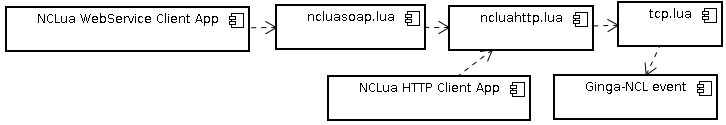
\includegraphics[width=0.8\textwidth]{ncluasoap-component-diagram.png}
	\captionof{figure}{Diagrama de Componentes do NCLua SOAP e NCLua HTTP}
	\label{fig:diagrama-componentes}
\end{center}

\begin{comment}
A Figura \ref{fig:class-diagram-ncluasoap-ncluahttp} apresenta um diagrama de classes
dos módulos implementados e suas dependências. Nele pode-se ver que são utilizados
mais dois módulos auxiliares: util e base64, o primeiro contendo funções de uso geral
e o outro contendo rotinas para codificação e decoficação de dados em formato base64,
utilizado, por exemplo, na criptografia da senha do usuário em requisições que requerem autentição HTTP.

\begin{center}
	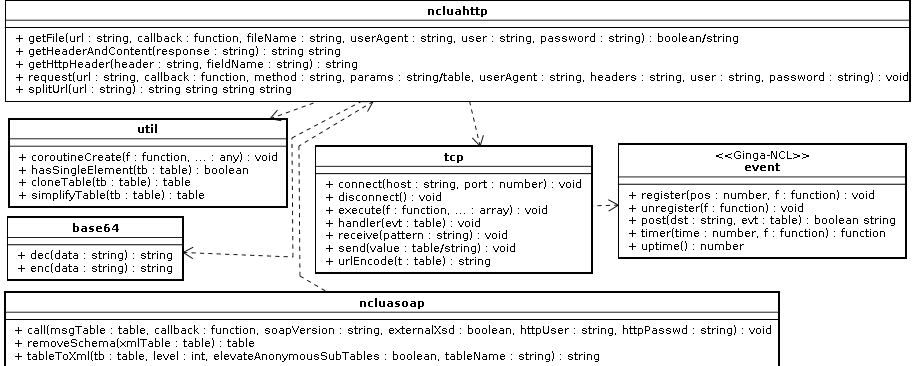
\includegraphics[width=0.9\textwidth]{ncluasoap-class-diagram.png}
	\captionof{figure}{Diagrama de Classes do NCLua SOAP e NCLua HTTP}
	\label{fig:class-diagram-ncluasoap-ncluahttp}
\end{center}
\end{comment}

\section{Exemplos de Uso e Testes de Interoperabilidade} \label{sec:resultados}

Nesta seção são apresentados os exemplos de utilização e aplicações desenvolvidas utilizando os módulos
NCLua HTTP e NCLua SOAP, bem como testes de interoperabilidade realizados.

\subsection{Exemplos de uso do NCLua HTTP}

A utilização básica do módulo NCLua HTTP é por meio de uma chamada \textit{GET}
a uma determinada URI\nomenclature{URI}{\textit{Uniform Resource Identifier}}, utilizando o método \textit{request} do módulo, como exemplificado no \textit{script}
NCLua da Listagem \ref{list:ncluahttp2}. Tal exemplo envia uma requisição HTTP \textit{GET} para a página
em \url{http://manoelcampos.com/votacao/votacao2.php}, enviando um parâmetro "voto" com valor igual a "sim",
obtendo o resultado (um código HTML neste caso) e exibindo no terminal. 
Não existe interface gráfica neste exemplo, 
desta forma, o \textit{script} contém apenas detalhes da requisição HTTP, mas é inteiramente funcional.

Na Listagem \ref{list:ncluahttp2}, a linha 1 adiciona o módulo NCLua HTTP. 
A linha 8 chama a função \textit{http.request}
que envia a requisição HTTP. Devido à particularidade assíncrona
do protocolo TCP no Ginga-NCL (que é utilizado para transportar as mensagens HTTP), como explicado na Seção \ref{sec:tcp},
para facilitar o envio de requisições e recebimento de respostas,
o módulo NCLua HTTP utiliza co-rotinas de Lua. 
Por este motivo, a obtenção do retorno deve ser feita dentro de uma função, como
a definida na linha 6, contendo os parâmetros header e body (comentados na definição
da mesma). Tal função deve ser passada como parâmetro à função \textit{http.request}, para que seja
chamada por esta quando a resposta for obtida. 

\begin{lstlisting}[caption=Exemplo de envio de requisição GET com NCLua HTTP, label=list:ncluahttp2, language=lua]
require "http"
---Funcao de callback executada de forma assincrona pelo modulo, 
--quando a resposta da requisicao eh obtida.
--@param header Headers HTTP enviados na resposta
--@param body Corpo da mensagem HTTP
function getResponse(header, body) print("Resposta obtida\n", body) end

http.request("http://manoelcampos.com/voto.php?voto=sim", getResponse)
\end{lstlisting}

O envio de requisições \textit{POST} é bastante semelhante ao exemplo apresentado anteriormente. 
Neste caso, os parâmetros devem ser passados à função \textit{http.request} por meio
de uma tabela Lua. A formatação destes valores, como exigido pelo protocolo HTTP, é feita automaticamente pelo NCLua HTTP.

Algumas aplicações foram desenvolvidas como prova de conceito do uso do módulo NCLua HTTP,
as quais são apresentadas a seguir:

\begin{itemize} 
	\item \textbf{Enquete TVD}: enquete com registro de voto e apuração a partir de servidor \textit{Web};
  \item \textbf{NCLua RSS Reader}: leitor de notícias RSS de um provedor de conteúdo na \textit{Web};
  \item \textbf{NCLua Tweet}: envio e recebimento de mensagens pelo micro \textit{blog Twitter}.
\end{itemize}

\subsection{Exemplos de uso do NCLua SOAP} \label{sec:apps-ncluasoap}

A seguir são apresentados exemplos de uso do NCLua SOAP para consumo de alguns \textit{Web Services}
disponíveis na \textit{Internet}.

A Listagem \ref{list:ncluasoap1} apresenta um exemplo de aplicação para exibir a previsão do tempo
de uma cidade. A mesma não possui interface gráfica, mostrando o resultado no terminal, para simplificar
o código. A linha 10 realiza a chamada ao método remoto. Os dados para realização da requisição
(incluindo o endereço do serviço, nome do método remoto e parâmetros de entrada) devem ser informados
em uma tabela Lua, como mostrado entre as linhas 4 a 8. A obtenção do retorno
do método remoto não é direta, devido à característica assíncrona do protocolo TCP
no Ginga-NCL, como já explanado nas Seções \ref{sec:tcp} e \ref{sec:ncluahttp}.
Desta forma, é necessária a definição de uma função que deve receber apenas um parâmetro
(normalmente nomeado de \textit{result}), como a função \textit{getResponse} exibida na linha 2. 
Tal função deve ser passada como parâmetro ao método \textit{call} do módulo ncluasoap,
como mostrado na linha 10. O envio da requisição será executado dentro de uma co-rotina Lua,
criada pelo NCLua SOAP. A função \textit{getResponse} será executada automaticamente quando o retorno for obtido.
Desta forma, todo o controle das chamadas assíncronas é feito pelo NCLua SOAP, como já 
amplamente discutido na Seção \ref{sec:ncluahttp}.

Como o serviço consumido neste exemplo retorna apenas uma \textit{string} com a previsão do tempo (chuvoso, nublado, ensolarado, etc),
para exibir tal resultado basta imprimir o parâmetro \textit{result} da função \textit{getResponse}, como 
apresentado na linha 6.

\begin{lstlisting}[caption=Exemplo de consumo de \textit{Web Service} de previsão do tempo, label=list:ncluasoap1, language=lua]
require "ncluasoap"
function getResponse(result) print("Previsao do Tempo: ", result) end

local msg = {
  address = "http://www.deeptraining.com/webservices/weather.asmx",
  namespace = "http://litwinconsulting.com/webservices/",
  operationName = "GetWeather", params = {  City = "New York"  }  
}

ncluasoap.call(msg, getResponse)
\end{lstlisting}

O exemplo apresentado na Listagem \ref{list:ncluasoap2} consume um serviço para obtenção de um endereço a partir do CEP.
Observe que o que muda entre as linhas 6 e 10, em relação ao exemplo anterior, são apenas os valores
da tabela "msg", que contém os dados para geração da requisição SOAP. Na função \textit{getResponse}, entre as linhas
2 e 4, note que agora, o resultado retornado é um tipo composto, que é acessado como uma tabela Lua.
Tal tabela conterá campos com os valores armazenados no XML enviado pelo \textit{Web Service}.

\begin{lstlisting}[caption=Exemplo de consumo de WS de consulta de endereço a partir do CEP, label=list:ncluasoap2, language=lua]
require "ncluasoap"
function getResponse(result)
   print(result.nome, result.bairro, result.cidade, result.UF)
end

local msg = {
  address = "http://www.bronzebusiness.com.br/webservices/wscep.asmx",
  namespace = "http://tempuri.org/",
  operationName = "cep", params = {  strcep = "70855530"  }  
}

ncluasoap.call(msg, getResponse)
\end{lstlisting}

Algumas aplicações foram desenvolvidas como prova de conceito de utilização do módulo.
Entre elas estão o rastreamento de encomendas postadas pelos Correios,
consulta de cotação do Dólar, previsão do tempo,
consulta de endereço a partir do CEP e outras.

\subsubsection{Testes de Interoperabilidade}

Os diversos serviços consumidos pelas aplicações apresentadas 
são desenvolvidos em diferentes linguagens e plataformas. Procurou-se realizar testes
com estes diferentes serviços para verificar a interoperabilidade do NCLua SOAP 
(um dos requisitos fundamentais, se não o mais importante, para qualquer implementação
SOAP). Com os testes realizados pôde-se comprovar a eficiência do módulo, uma vez que para todos
os serviços testados, obteve-se o retorno esperado, tratando-o de forma padronizada.

No início, alguns usuários do fórum do projeto relataram problemas ao utilizar serviços
desenvolvidos em linguagem Java. Os problemas encontrados foram
devido aos \textit{Web Services} criados com a API JAX-WS, padrão da plataforma Java,
especificarem os tipos de dados utilizados pelo serviço em um arquivo XSD (\textit{XML Schema Definition}) externo,
no lugar de especificar diretamente dentro do documento WSDL. 
Tal característica requer pequenas mudanças no formato da mensagem SOAP
a ser enviada para consumir tais \textit{Web Services}. Assim, foi
preciso adequar o módulo para entrar em conformidade com o padrão SOAP.

Particularidades encontradas em \textit{Web Services} PHP também foram relatadas
e o módulo foi adequado para permitir a interoperabilidade com tais serviços.
É importante ressaltar que, no caso de tais serviços PHP, estes foram desenvolvidos
utilizando o \textit{tookit} nuSOAP\footnote{\url{http://sourceforge.net/projects/nusoap}}.
Tal \textit{tookit} não leva em conta os nomes dos parâmetros de entrada e sim a ordem
dos mesmos, não estando em conformidade com o padrão SOAP. Assim, o problema é específico da implementação
do nuSOAP, mas que foi contornado pelo NCLua SOAP para evitar quaisquer transtornos
ao consumir \textit{Web Services} desenvolvidos com tal \textit{tookit}. 

 %input no lugar de include evita a quebra de linha inserida por este
%\section{Limitações do módulo NCLua SOAP}



\chapter{Conclusões e Trabalhos Futuros} \label{cap:conclusao}

\section{Conclusões}

\added{As implementações apresentadas nesta dissertação são todas originais, por
não haver nenhuma outra implementação (pelo menos de código aberto)
para o sub-sistema Ginga-NCL dos protocolos HTTP e SOAP, de
um \textit{framework} de componentes gráficos e de aplicações de
\textit{T-Commerce}. Tais implementações permitem o desenvolvimento
de aplicações dos mais variados tipos para o Ginga-NCL, alavancando
o desenvolvimento de aplicações interativas para o SBTVD (ISDB-TB).}

Os módulos NCLua HTTP e NCLua SOAP facilitam a convergência entre \textit{Web} e TV, escondendo
os detalhes de implementação dos protocolos HTTP e SOAP do desenvolvedor
de aplicações de TVDi, permitindo o surgimento de novas aplicações interativas 
que fazem uso de conteúdo da \textit{Internet}.
O NCLua SOAP permitiu o desenvolvimento de aplicações de \textit{T-Government}
como apresentado em \cite{tgov2010barbosa}, sistema de recomendação\cite{gatto2010BIPODiTVR} entre outras. 
Na página do projeto, em http://ncluasoap.manoelcampos.com,
existe um \textit{link} para o fórum de discussão do módulo, onde alguns usuários relatam a
utilização do mesmo, por exemplo, em aplicações de \textit{T-Learning}.

Atualmente, o processo de obtenção dos dados para realizar a chamada a um método remoto em um \textit{Web Service}
ainda é praticamente todo manual, no entanto, 
após o desenvolvedor obter tais dados para o método remoto desejado, a realização da requisição é bastante simplificada,
principalmente pelo fato de Lua ser uma linguagem de tipagem dinâmica \cite{ierusalimschy2006programming}, 
não obrigando a declaração de variáveis com seus respectivos tipos.
O \textit{feedback} dos usuários tem mostrado que o módulo está sendo bastante útil para 
a comunidade, além de permitir a evolução do mesmo.


%\textbf{APRESENTAR CONCLUSÕES A AVALIAÇÕES DE RESULTADOS DA ARQUITETURA E DA APP DE T-COMMERCE}

A arquitetura proposta serve de base para o desenvolvimento de serviços de \textit{T-Commerce} para o SBTVD,
mostrando como diversos serviços podem ser integrados em uma única arquitetura para um propósito final.
Tal arquitetura também serve como um estudo de caso dos percalços enfrentados para a elaboração
de um ambiente de desenvolvimento e testes de aplicações para o SBTVD, mostrando
as ferramentas necessárias para isto.

As análises de desempenho apresentadas dos protocolos implementados mostraram como a solução proposta
é eficiente em uso de processador e memória RAM, sendo uma solução ideal para uso em 
ambientes restritos de recursos, como os \textit{Set-top Boxes}.

Os protocolos implementados são a base da integração entre \textit{Web} e TV
e estão sendo bastante úteis em diversos outros trabalhos, como apresentado
no Capítulo \ref{cap:ncluasoap}, mostrando como os resultados alcançados se tornaram
importantes para a comunidade de TV Digital no Brasil e na América Latina, 
onde quase todos os países já adotaram o ISDB-TB.

A aplicação de \textit{T-Commerce} desenvolvida delineia o processo de desenvolvimento
de aplicações que fogem do trivial, mostrando como aplicar recursos como orientação
a objetos na linguagem Lua, \added{uso do canal de retorno/interatividade no SBTVD, 
uso de arquivos XML e arquivos de dados em formato Lua, além de outros recursos}. 
O uso do \textit{framework} LuaOnTV para construção
de interfaces gráficas de usuário é bastante flexível e dá suporte a múltiplos
dispositivos, adaptação automática das dimensões dos componentes gráficos
da aplicação, além do uso de \textit{templates} para permitir uma 
definição centralizada da identidade visual da aplicação.
Tal recurso de \textit{templates} permite alterar a identidade visual da aplicação facilmente, 
podendo-se ter \textit{templates} diferentes para tipos de dispositivos diferentes (como TV's e celulares).

Outras aplicações foram desenvolvidas, como o NCLua RSS \textit{Reader} e o Rastreador de Encomendas
que servem como prova de conceito dos protocolos como HTTP e SOAP, implementados nesta dissertação.

Os objetivos apresentados na Seção \ref{sec:objetivos} foram todos alcançados,
apresentando uma solução completa, desde o ambiente de desenvolvimento, até 
a realização de análises de desempenho das aplicações desenvolvidas.

\added{
A Tabela \ref{tab:obj-espec-alcancados} apresenta uma descrição de como tais objetivos foram alcançados.
\begin{center}
	\begin{tabular}{|p{2cm}|p{13cm}|}
	  \hline 
		\textbf{Objetivo Específico} & \textbf{Como foi alcançado} \\
		\hline 
		A & Os requisitos funcionais e não funcionais foram elicitados, tendo
		servido de guia para o desenvolvimento da arquitetura proposta; \\
		\hline 
		B & a arquitetura foi proposta e desenvolvida, apresentando-se
		a mesma por meio de figuras e diagramas UML, além da montagem de uma
		distribuição GNU/Linux contendo todo o ambiente de desenvolvimento elaborado;  \\	
		\hline 
		C & um \textit{framework} de comunicação de dados foi desenvolvido, composto
		pelos módulos NCLua HTTP e NCLua SOAP, que implementam os protocolos HTTP e SOAP, respectivamente,
		sendo a base de toda a interoperação das aplicações desenvolvidas com diferentes provedores de serviços \textit{Web}; \\
		\hline 
		D & as diferentes aplicações de TVDi propostas foram desenvolvidas e apresentadas, servindo como prova
		de conceito do uso dos \textit{frameworks} desenvolvidos ou estendidos; \\
		\hline 
		E & o \textit{framework} LuaOnTV foi estendido, incluindo-se suporte a temas. O recurso
		de temas foi utilizado na aplicação de \textit{T-Commerce} desenvolvida. 
		A adaptação automática da interface da aplicação foi testada em ambiente
		virtual de TV Digital (o Ginga \textit{Virtual Set-top Box}) 
		com diferentes resoluções de tela. Em tal ambiente, a adaptação automática do tamanho
		da interface gráfica da aplicação ao tamanho da tela do televisor
		mostrou-se satisfatória, possibilitando que a aplicação de adapte automaticamente
		a diferentes dispositivos receptores de TVD; \\
		\hline 
		F & um modelo de desenvolvimento de aplicações de TVDi baseado em \textit{templates}
		foi elaborado e apresentado. Tal modelo foi utilizado na aplicação de \textit{T-Commerce} desenvolvida,
		o que permitiu uma agilidade no desenvolvimento da mesma, definindo
		um conjunto de componentes gráficos básicos e uma identidade visual
		comum a todas as telas da aplicação desenvolvida.\\								
		\hline 
	\end{tabular}
	\captionof{table}{Objetivos Específicos Alcançados}
	\label{tab:obj-espec-alcancados}
\end{center}
}

\section{Trabalhos Futuros}

Como trabalhos futuros, pretende-se concluir a implementação do \textit{parse} automático do 
documento WSDL e geração de \textit{stubs} Lua, contendo funções \textit{proxies} para realizar a chamada aos métodos remotos
(semelhante a ferramentas como o \textit{wsdl2java}\footnote{http://ws.apache.org/axis/java/user-guide.html}, 
pretende-se transformar o \textit{script} \textit{wsdlparser} em um \textit{wsdl2nclua})
e incluir tratamento de exceções para permitir que as aplicações
de TVDi possam emitir mensagens amigáveis ao usuário quando uma requisição HTTP falhar.

O módulo NCLua HTTP permite que seja utilizado qualquer método HTTP em uma requisição, no entanto,
apenas os método \textit{GET} e \textit{POST} foram testados. Desta forma, pretende-se realizar testes
de conformidade utilizando-se os métodos HTTP \textit{OPTIONS, HEAD, PUT} e \textit{DELETE}. Pretende-se também
implementar mais funcionalidades no módulo, como realizar redirecionamentos automaticamente
a partir de respostas HTTP como 301 e 302, além de implementar alguns recursos do HTTP/1.1, como
conexões persistentes.



A arquitetura também pode ser estendida nos pontos a seguir:

\begin{itemize}
	\item incluir suporte a metadados na aplicação para que a
mesma possa oferecer produtos vinculados
a um programa televisivo, permitindo que
a oferta do produto seja mostrada 
ao telespectador em momento determinado no
arquivo de metadados, utilizando os recursos
de sincronização de mídias existente na linguagem NCL;
   \item estudar a viabilidade e uso do protocolo de autorização \textit{Open Authentication} (oAuth)\footnote{\url{http://oauth.net}},
que é bastante utilizado atualmente em redes sociais,
permitindo ao usuário ter um login e senha únicos para acesso a diferentes serviços,
agilizando o processo de login (caso o usuário decida salvar localmente, de forma criptografada, 
as informações de autorização);
   \item estender a arquitetura para um modelo baseado em descoberta de serviços que
possibilite a integração de diferentes lojas virtuais
que implementem a arquitetura aqui proposta,
utilizando recursos como a linguagem BPEL (\textit{Business Process Execution Language})\nomenclature{BPEL}{\textit{Business Process Execution Language}}
para permitir a composição de serviços e tornar tal integração transparente para aplicação de TVDi;
  \item utilizar a extensão \textit{WS-Security}\cite{oasis-wssecurity} para permitir a segurança na comunicação entre os \textit{Web Services} e as aplicações cliente;
  \item criar ferramenta, para execução do lado da emissora de TV, que permita o envio dos produtos em oferta
  via \textit{broadcast}, possibilitando a usuários, sem conexão com a \textit{Internet}, visualizarem tais produtos
  na tela de seu equipamento de TVD.
\end{itemize}



%\bibliographystyle{abnt-num} % use este estilo para ABNT numerico
\bibliographystyle{abnt-alf} % use este estilo para ABNT alfabético
%\bibliographystyle{sbc}

%\renewcommand{\bibname}{REFERÊNCIAS BIBLIOGRÁFICAS} %Define o Caption da seção de bibliografia
%\addcontentsline{toc}{chapter}{REFERÊNCIAS BIBLIOGRÁFICAS} %????????????????????

%não pode ter espaço entre os nomes dos arquivos bib
\bibliography{referencias,referencias-artigo}

\chapter*{Apêndice \added{A}}
\addcontentsline{toc}{chapter}{Apêndice A}

\section*{\textit{Screenshots} da aplicação de \textit{T-Commerce}}
\addcontentsline{toc}{section}{Screenshots da aplicação de \textit{T-Commerce}}

\begin{center}
	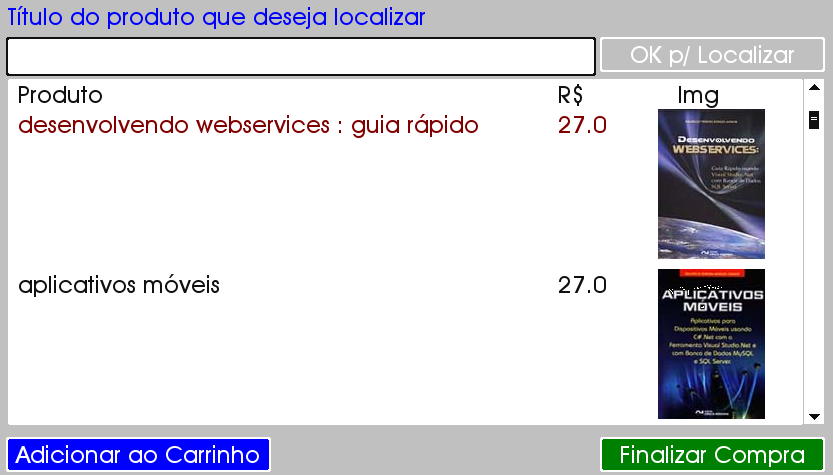
\includegraphics[width=0.93\textwidth]{CommerceApp/TCommerce-App-Destaques.png}
	\captionof{figure}{Aplicação de \textit{T-Commerce}: Tela inicial com produtos em destaque}
\end{center}

\begin{center}
	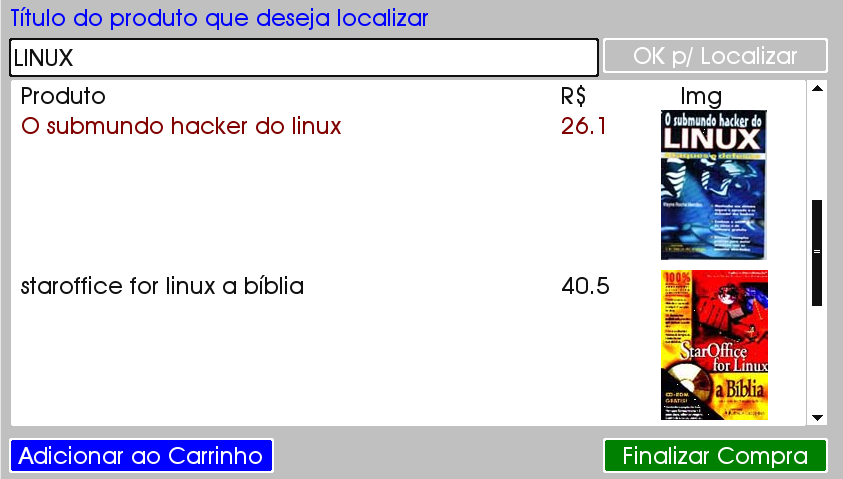
\includegraphics[width=0.93\textwidth]{CommerceApp/TCommerce-App-BuscaProdutos.png}
	\captionof{figure}{Aplicação de \textit{T-Commerce}: Busca de produtos}
\end{center}

\begin{center}
	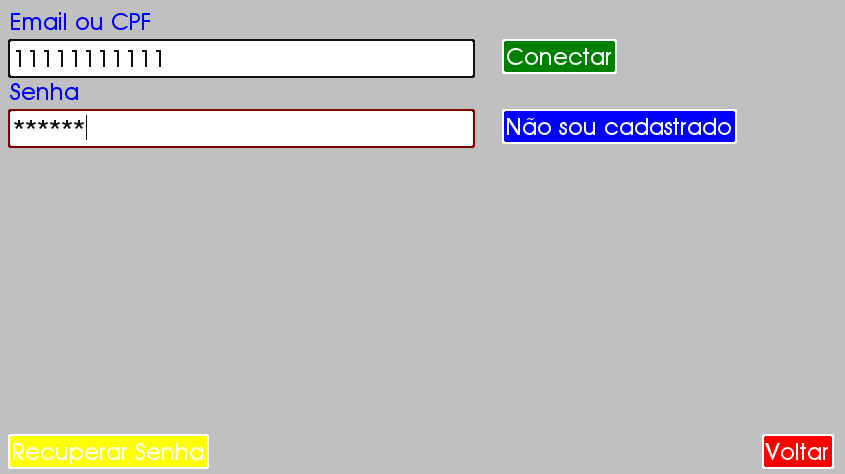
\includegraphics[width=0.94\textwidth]{CommerceApp/TCommerce-App-Login.png}
	\captionof{figure}{Aplicação de \textit{T-Commerce}: Login (utilizando \textit{e-mail} ou CPF)}
\end{center}

\begin{center}
	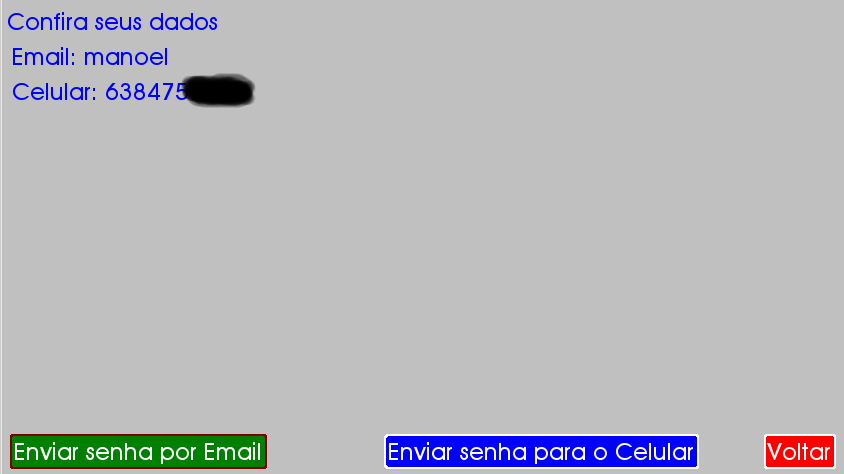
\includegraphics[width=0.94\textwidth]{CommerceApp/TCommerce-App-Recuperar-Senha.png}
	\captionof{figure}{Aplicação de \textit{T-Commerce}: Recuperar senha por \textit{e-mail} ou SMS}
\end{center}

\begin{center}
	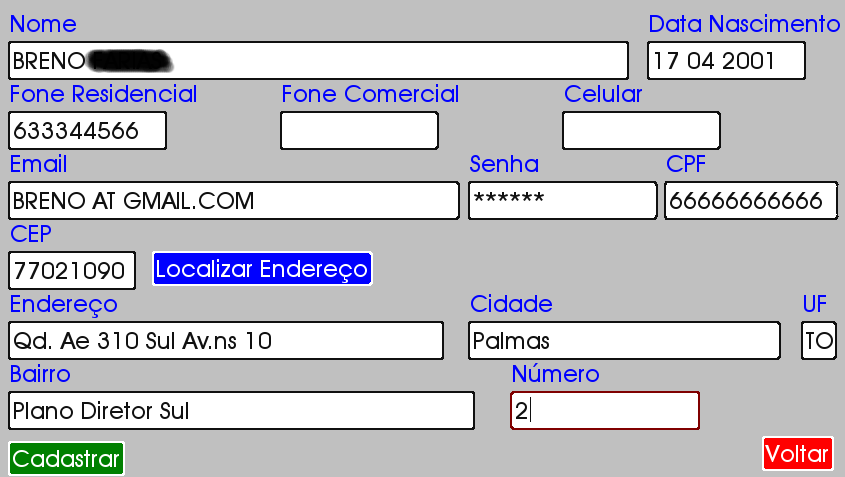
\includegraphics[width=0.94\textwidth]{CommerceApp/TCommerce-App-Cadastro-Cliente.png}
	\captionof{figure}[Aplicação de \textit{T-Commerce}: Cadastro de Clientes]{Aplicação de \textit{T-Commerce}: Cadastro de Clientes (com busca de endereço a partir do CEP)}
\end{center}

\begin{center}
	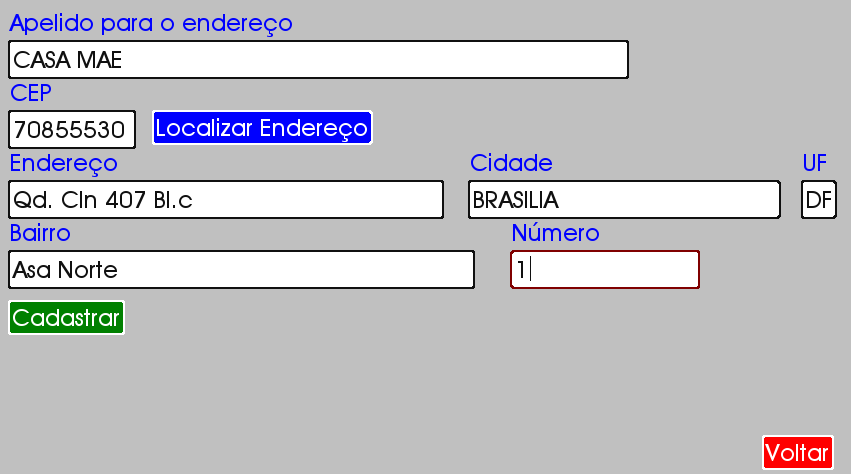
\includegraphics[width=0.94\textwidth]{CommerceApp/TCommerce-App-Cadastro-Endereco.png}
	\captionof{figure}[Aplicação de \textit{T-Commerce}: Cadastro de Endereços]{Aplicação de \textit{T-Commerce}: Cadastro de Endereços (com busca de endereço a partir do CEP)}
\end{center}

\begin{center}
	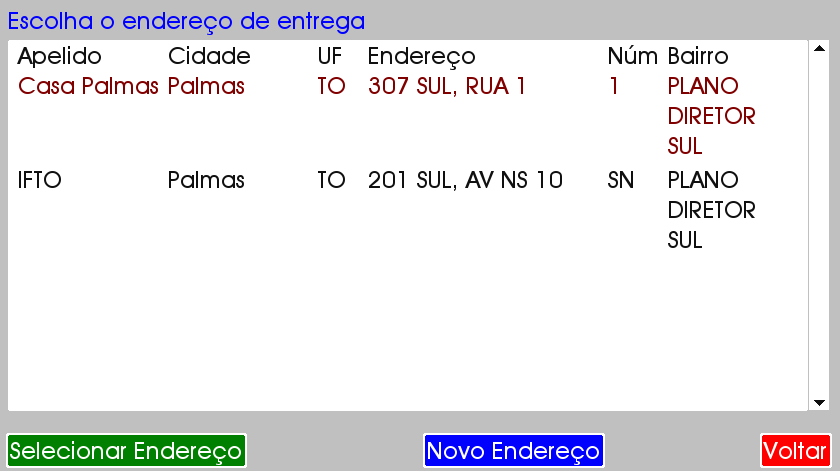
\includegraphics[width=0.94\textwidth]{CommerceApp/TCommerce-App-Selecao-Endereco.png}
	\captionof{figure}{Aplicação de \textit{T-Commerce}: Seleção de Endereços}
\end{center}

\begin{center}
	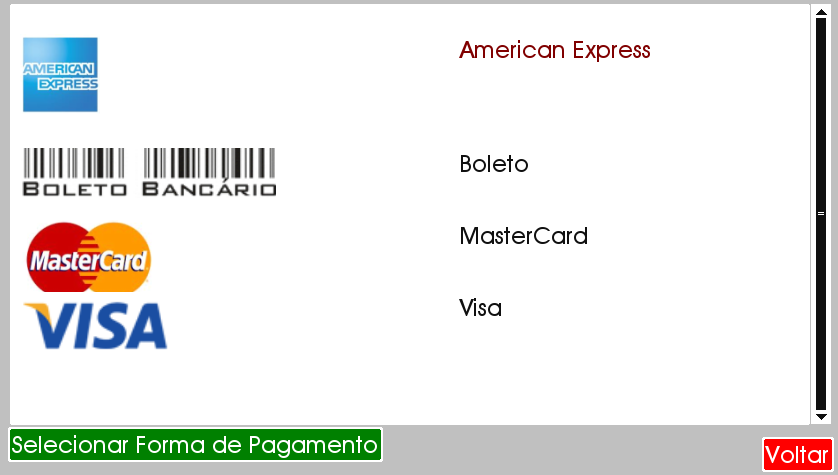
\includegraphics[width=0.94\textwidth]{CommerceApp/TCommerce-App-Forma-Pagamento.png}
	\captionof{figure}{Aplicação de \textit{T-Commerce}: Formas de Pagamento}
\end{center}

\begin{center}
	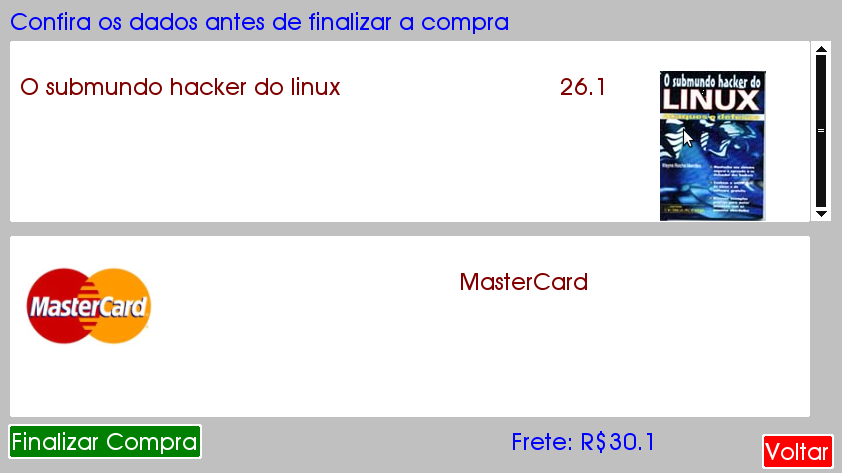
\includegraphics[width=0.94\textwidth]{CommerceApp/TCommerce-App-Finalizar-Compra.png}
	\captionof{figure}{Aplicação de \textit{T-Commerce}: Finalizar Compra}
\end{center}


\begin{comment}
\section*{Publicações}
%\addcontentsline{toc}{section}{Publicações}
\newpage
\end{comment}


\end{document}
